% ============================================================
%  PE5 -- Unidad 5 | PLANTILLA DE TRABAJO DIVIDIDO
%  MundiPets -- Plataforma de Adopción y Cruza Responsable de Mascotas
%  Asignatura: Ingeniería de Requisitos (ISR-401) -- UTEQ 2026-2027 PPA
%  Formato: IEEE onecolumn | Biber + biblatex (estilo IEEE)
%  Preámbulo trasplantado y adaptado del ERS_SRS_2B_v2_0.tex del PFC,
%  para que la PE5 y el ERS compartan exactamente el mismo motor de
%  compilación (mismo compilador, mismo estilo de citas, misma
%  numeración de tablas/figuras). Ver Sección 0.6 y 0.7 del cuerpo.
%
%  COMO USAR ESTE ARCHIVO
%  ----------------------
%  Cada bloque  indica QUE debe producir un
%  integrante en esa sección. El responsable borra la caja 
%  y la reemplaza por el contenido real. Cuando no quede ninguna caja
%  gris en el documento, la PE5 está terminada.
%
%  COMPILACIÓN (requiere referencias.bib en la misma carpeta):
%      pdflatex PE5_U5_Trabajo_Dividido.tex
%      biber    PE5_U5_Trabajo_Dividido
%      pdflatex PE5_U5_Trabajo_Dividido.tex
%      pdflatex PE5_U5_Trabajo_Dividido.tex
% ============================================================
\documentclass[journal,onecolumn]{IEEEtran}

% ── Codificación e idioma ───────────────────────────────────
\usepackage[T1]{fontenc}
\usepackage[utf8]{inputenc}
\usepackage[spanish, es-tabla]{babel}
\usepackage[autostyle=true, spanish=mexican]{csquotes}
\usepackage[htt]{hyphenat}   % permite guionar dentro de \texttt (evita Overfull)

% ── Tablas ──────────────────────────────────────────────────
\usepackage{booktabs}
\usepackage{tabularx}
\usepackage{array}
\usepackage{multirow}
\usepackage{longtable}
\newcolumntype{C}[1]{>{\centering\arraybackslash}p{#1}}
\newcolumntype{L}[1]{>{\raggedright\arraybackslash}p{#1}}
\renewcommand{\thetable}{\arabic{table}}
\def\tablename{Tabla}

% ── Figuras ─────────────────────────────────────────────────
\usepackage{graphicx}
\graphicspath{{figuras/}{./}}
\usepackage{float}
\usepackage{pdflscape}   % matriz de trazabilidad en horizontal

% ── Color ───────────────────────────────────────────────────
\usepackage{xcolor}
\definecolor{uteqverde}{RGB}{0,110,60}
\definecolor{codegray}{gray}{0.95}
\definecolor{codegreen}{rgb}{0.0,0.5,0.0}
\definecolor{codeblue}{rgb}{0.0,0.0,0.6}
\definecolor{codepurple}{rgb}{0.5,0.0,0.35}

% ── Geometría ───────────────────────────────────────────────
\usepackage{geometry}
\geometry{a4paper, top=2.5cm, bottom=2.5cm, left=2.5cm, right=2.5cm,
	headheight=14pt, footskip=1.2cm}

% ── Encabezado y pie ────────────────────────────────────────
\usepackage{fancyhdr}
\pagestyle{fancy}
\fancyhf{}
\renewcommand{\headrulewidth}{0.4pt}
\fancyhead[L]{\small PE5 -- Unidad 5 -- Ingeniería de Requisitos}
\fancyhead[R]{\small MundiPets -- Trabajo dividido}
\fancyfoot[C]{\thepage}

% ── Espaciado y listas ──────────────────────────────────────
\usepackage{parskip}
\setlength{\parskip}{4pt}
\setlength{\emergencystretch}{3em}   % tolerancia extra de línea
\makeatletter
\@ifundefined{labelindent}{}{\let\labelindent\relax}
\makeatother
\usepackage{enumitem}
\usepackage{amssymb}
\usepackage{amsmath}

% ── Títulos de sección ──────────────────────────────────────
\usepackage{titlesec}
\renewcommand{\thesection}{\arabic{section}}
\renewcommand{\thesubsection}{\thesection.\arabic{subsection}}
\renewcommand{\thesubsubsection}{\thesubsection.\arabic{subsubsection}}
\titleformat{\section}{\normalfont\Large\bfseries}{\thesection}{1em}{}
\titleformat{\subsection}{\normalfont\large\bfseries}{\thesubsection}{1em}{}
\titleformat{\subsubsection}{\normalfont\normalsize\bfseries}{\thesubsubsection}{1em}{}
\setcounter{secnumdepth}{4}
\setcounter{tocdepth}{4}

% ── Leyendas ────────────────────────────────────────────────
\usepackage{caption}
\captionsetup{font=small, labelfont=bf}

% ── Bibliografía (biber + estilo IEEE) ──────────────────────
% Mismo motor que el ERS del PFC: ver Sección 0.6 y 0.7 del cuerpo
% para el orden exacto de compilación.
\usepackage[
backend=biber,
style=ieee,
citestyle=numeric-comp,
isbn=true,
doi=true
]{biblatex}
\addbibresource{referencias.bib}

% ── Enlaces ─────────────────────────────────────────────────
\usepackage[hidelinks,colorlinks=false]{hyperref}
\usepackage{url}

% ============================================================
%  CAJA DE GUÍA (fondo gris claro, borde negro)
% ============================================================
\usepackage{mdframed}
\mdfdefinestyle{guia}{
	linecolor=black,
	linewidth=0.6pt,
	backgroundcolor=gray!10,
	innertopmargin=6pt,
	innerbottommargin=6pt,
	innerleftmargin=8pt,
	innerrightmargin=8pt,
	skipabove=4pt,
	skipbelow=4pt
}

% 
\newcommand{\guia}[2]{%
	\begin{mdframed}[style=guia]
		\noindent\textbf{Responsable: #1}\\[2pt]
		\textit{#2}
	\end{mdframed}
}

% -- Atajos de nombres (evita erratas al repetirlos) ---------
\newcommand{\rFUE}{FUERTES ARRAES, Edson Daniel}
\newcommand{\rGUT}{GUTIÉRREZ ORTEGA, Génesis Adriana}
\newcommand{\rMEN}{MENDOZA PÁRRAGA, Andy Johel}
\newcommand{\rMOR}{MORALES SÁNCHEZ, Gary Alejandro}
\newcommand{\rNIE}{NIEVES SÁNCHEZ, Jimmy Samuel}
\newcommand{\rTODOS}{TODO EL EQUIPO}

% ============================================================
\begin{document}

% ============================================================
%  PORTADA MINIMA DE ESTE FRAGMENTO INDIVIDUAL
%  Este archivo contiene unicamente las secciones bajo
%  responsabilidad de MORALES SANCHEZ, Gary Alejandro:
%  Fundamento Teorico (FT.3), Seccion 4 (Modelos UML del
%  Sistema) y Seccion 6 (Gestion y Trazabilidad). Se integra
%  al documento final del equipo (PE5_U5_Trabajo_Dividido.tex).
% ============================================================
\begin{center}
	{\Large\bfseries MundiPets --- PE5 Unidad 5}\\[4pt]
	{\large Fundamento Teórico (FT.3), Sección 4 y Sección 6}\\[4pt]
	{\normalsize Ingeniería de Requisitos (ISR-401) --- UTEQ 2026--2027 PPA}\\[12pt]
	{\normalsize Responsable: Morales Sánchez, Gary Alejandro}
\end{center}

\vspace{1cm}

% ============================================================
%  FUNDAMENTO TEORICO -- FT.3 (Morales)
% ============================================================
\section*{Fundamento Teórico}
\addcontentsline{toc}{section}{Fundamento Teórico}
\label{sec:fundamento_teorico}

\subsection*{Fundamentos de la trazabilidad y el modelado}
\addcontentsline{toc}{subsection}{Fundamentos de trazabilidad (Morales)}

El planteamiento seminal de Gotel y Finkelstein \cite{gotel1994}
identificó que buena parte de los problemas prácticos de trazabilidad no
surgen de una técnica insuficiente para vincular artefactos, sino de una
falta de acuerdo previo sobre qué tipo de trazabilidad se está
exigiendo. Los autores separan el problema en dos direcciones
complementarias: la trazabilidad previa a la especificación, que vincula
un requisito hacia atrás con la evidencia que lo originó, ya sea una
entrevista, una observación o una norma legal; y la trazabilidad
posterior a la especificación, que lo vincula hacia adelante con aquello
en lo que ese requisito se transforma durante el desarrollo, como un
caso de uso, una clase o un caso de prueba. Esta distinción sustenta
directamente la columna Fuente y la columna Estado de la traza de la
matriz del punto 6.2 de este informe: la primera resuelve la pregunta de
dónde nació este requisito, y la segunda, la pregunta de en qué se
convirtió; sin esa separación conceptual, ambas preguntas tienden a
mezclarse en una sola verificación superficial que no detecta en cuál de
las dos direcciones falla realmente la cadena.

La revisión sistemática más reciente de Mucha, Kaufmann y Riehle
\cite{mucha2024}, basada en el análisis de setenta y siete estudios
publicados entre 1992 y 2022, retoma específicamente la mitad de ese
marco correspondiente a la trazabilidad previa a la especificación,
señalada por los propios autores como la menos estudiada de las dos, y
documenta de forma sistemática los problemas recurrentes que enfrenta un
equipo al intentar mantenerla vigente durante todo el ciclo de vida del
proyecto. Entre esos problemas se encuentran precisamente las dos
patologías que este informe debió diagnosticar y cerrar en la Sección
6.3: la cadena rota, cuando un artefacto de diseño, como un caso de uso
o una clase, se construye sin que ningún requisito lo respalde
realmente, señal de alcance no solicitado; y el requisito huérfano,
cuando un requisito carece de fuente identificable o de cualquier
artefacto posterior que lo realice, señal de que fue documentado sin
evidencia suficiente o abandonado tras su especificación. Que estas
patologías aparezcan documentadas de forma independiente en la
literatura de trazabilidad, y no solo como una ocurrencia particular de
este proyecto, respalda que su tratamiento en la Sección 6.3 no fue un
ejercicio cosmético, sino la aplicación de un problema ya caracterizado
formalmente en la disciplina.

La cadena mínima que exige la PE5, compuesta por Fuente, RF, CU, Clase,
Estado, Criterio BDD y Caso de Prueba, es en consecuencia la aplicación
directa de este marco al proyecto MundiPets: sus primeros dos eslabones,
Fuente y RF, instancian la trazabilidad previa a la especificación de
Gotel y Finkelstein, y los eslabones restantes, desde RF hasta el Caso
de Prueba pasando por CU, Clase, Estado y Criterio BDD, instancian su
trazabilidad posterior a la especificación. Verificar ambas direcciones
en una sola matriz, en lugar de documentar solamente el origen de los
requisitos o solamente su realización en los modelos de la Sección 4, es
lo que permite detectar tanto las cadenas rotas como los huérfanos que
describen Mucha et al., y es exactamente el criterio bajo el cual se
construyeron y depuraron la lectura interpretativa de los modelos UML de
la Sección 4 y la matriz final del punto 6.2.

\newpage

\section{Modelos UML del Sistema}
	
	Esta sección presenta los modelos vigentes de la PE3 ya corregidos, con una
	lectura interpretativa de la decisión de diseño que refleja cada uno, no
	una descripción de lo que se observa en el dibujo. El orden sigue el
	recorrido natural del sistema: primero los modelos generales de alcance y
	arquitectura (casos de uso, contexto, componentes, despliegue) y los
	modelos estratégicos i* (SD y SR); luego el comportamiento dinámico
	(máquinas de estado, secuencia, actividad); y finalmente la estructura
	estática (clases).
	
	% ------------------------------------------------------------
	\subsection{Diagrama de Casos de Uso}
	
	\begin{figure}[H]
		\centering
		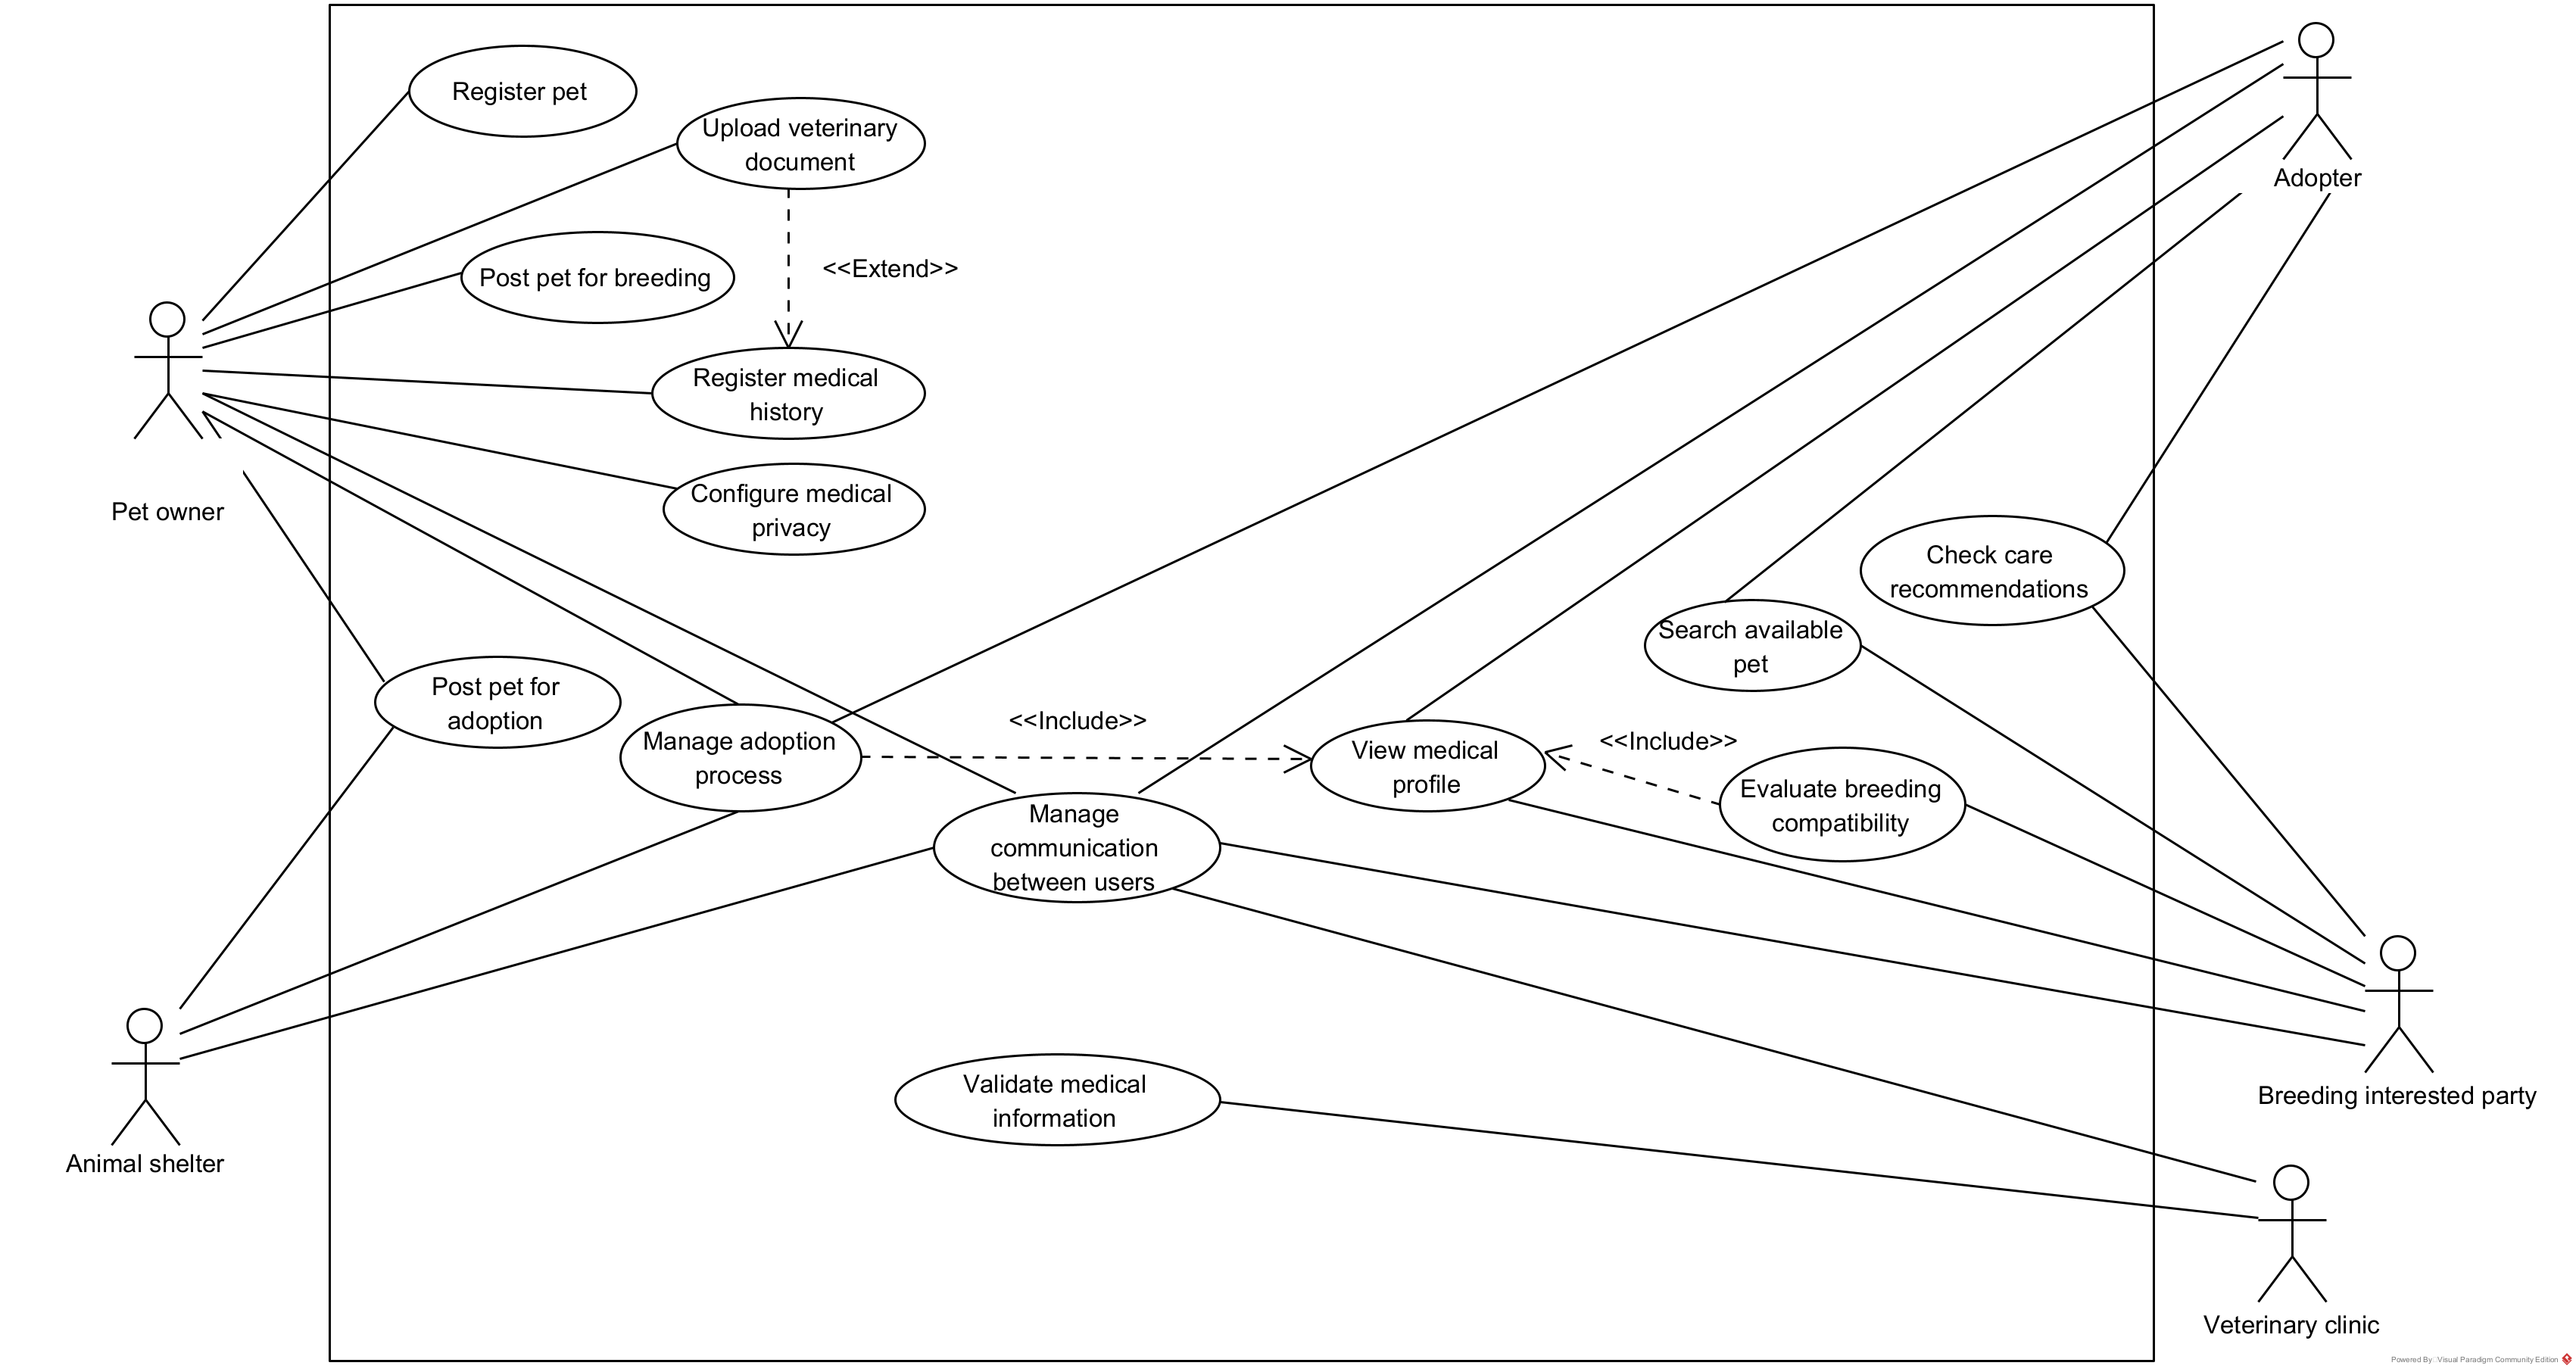
\includegraphics[width=0.95\textwidth]{DiagramaCasosDeUso_MundiPets.png}
		\caption{Diagrama de casos de uso general del sistema MundiPets.}
		\label{fig:cu_general}
	\end{figure}
	
	En la Figura~\ref{fig:cu_general}, la inclusión obligatoria de ``Manage
	adoption process'' y ``Manage communication between users'' hacia ``View
	medical profile'' refleja que ningún adoptante o interesado en cruza puede
	avanzar en una negociación sin pasar primero por el historial médico de la
	mascota: la transparencia sanitaria no es opcional, es un paso obligado
	del flujo. Por otro lado, ``Upload veterinary document'' extiende a
	``Register medical history'' (no lo incluye), lo que indica que adjuntar
	el documento formal es un enriquecimiento posterior y no una condición
	para registrar el historial básico, permitiendo que el dueño registre
	datos médicos mínimos, aunque aún no tenga el certificado en mano.
	
	% ------------------------------------------------------------
	\subsection{Diagrama de Contexto}
	
	\begin{figure}[H]
		\centering
		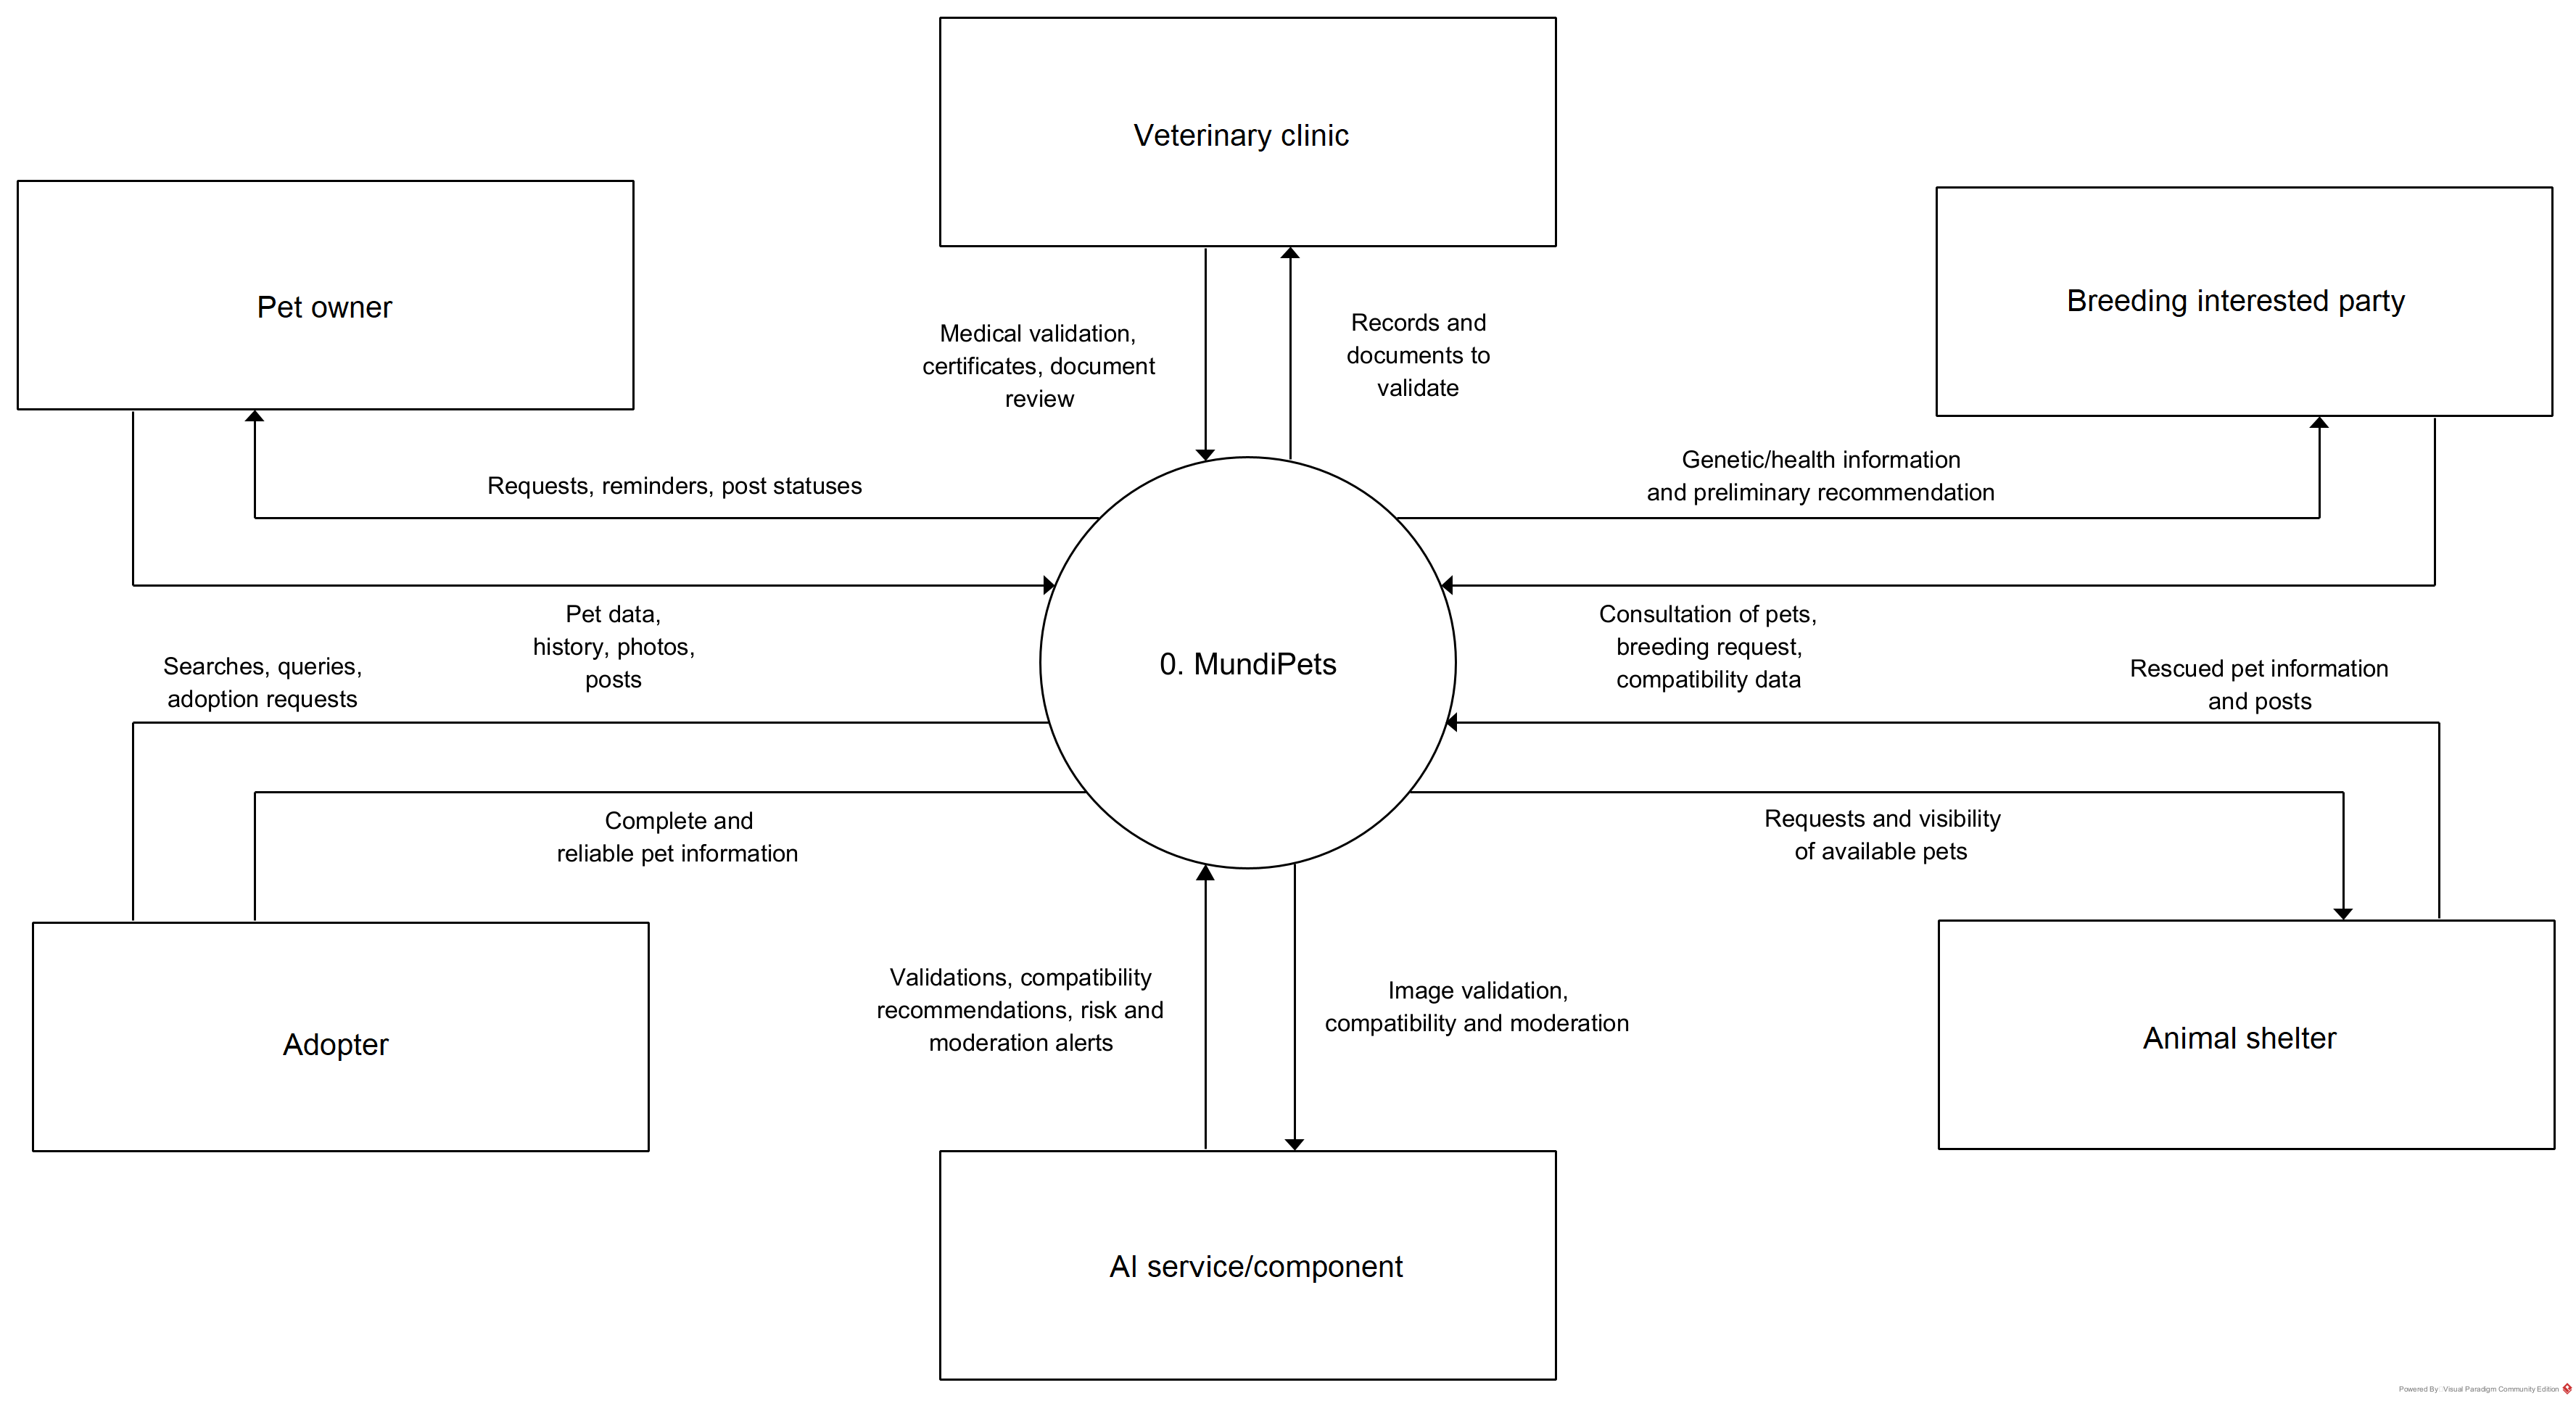
\includegraphics[width=0.95\textwidth]{DiagramaContexto_MundiPets.png}
		\caption{Diagrama de contexto del sistema MundiPets.}
		\label{fig:contexto}
	\end{figure}
	
	Como se observa en la Figura~\ref{fig:contexto}, la existencia de un actor
	externo independiente ``AI service/component'', con flujo bidireccional
	propio hacia el núcleo ``0. MundiPets'' (envía moderación de imágenes y
	compatibilidad, recibe validaciones), refleja la decisión de tratar la
	inteligencia artificial como un límite del sistema desacoplado del resto
	de actores humanos, y no como una función interna invisible. Esto
	anticipa que los componentes de IA (Sección~\ref{sec:req_ia}) tienen
	contratos de entrada/salida propios y auditables, no una lógica difusa
	mezclada con el resto del sistema.
	
	% ------------------------------------------------------------
	\subsection{Diagrama de Componentes}
	
	\begin{figure}[H]
		\centering
		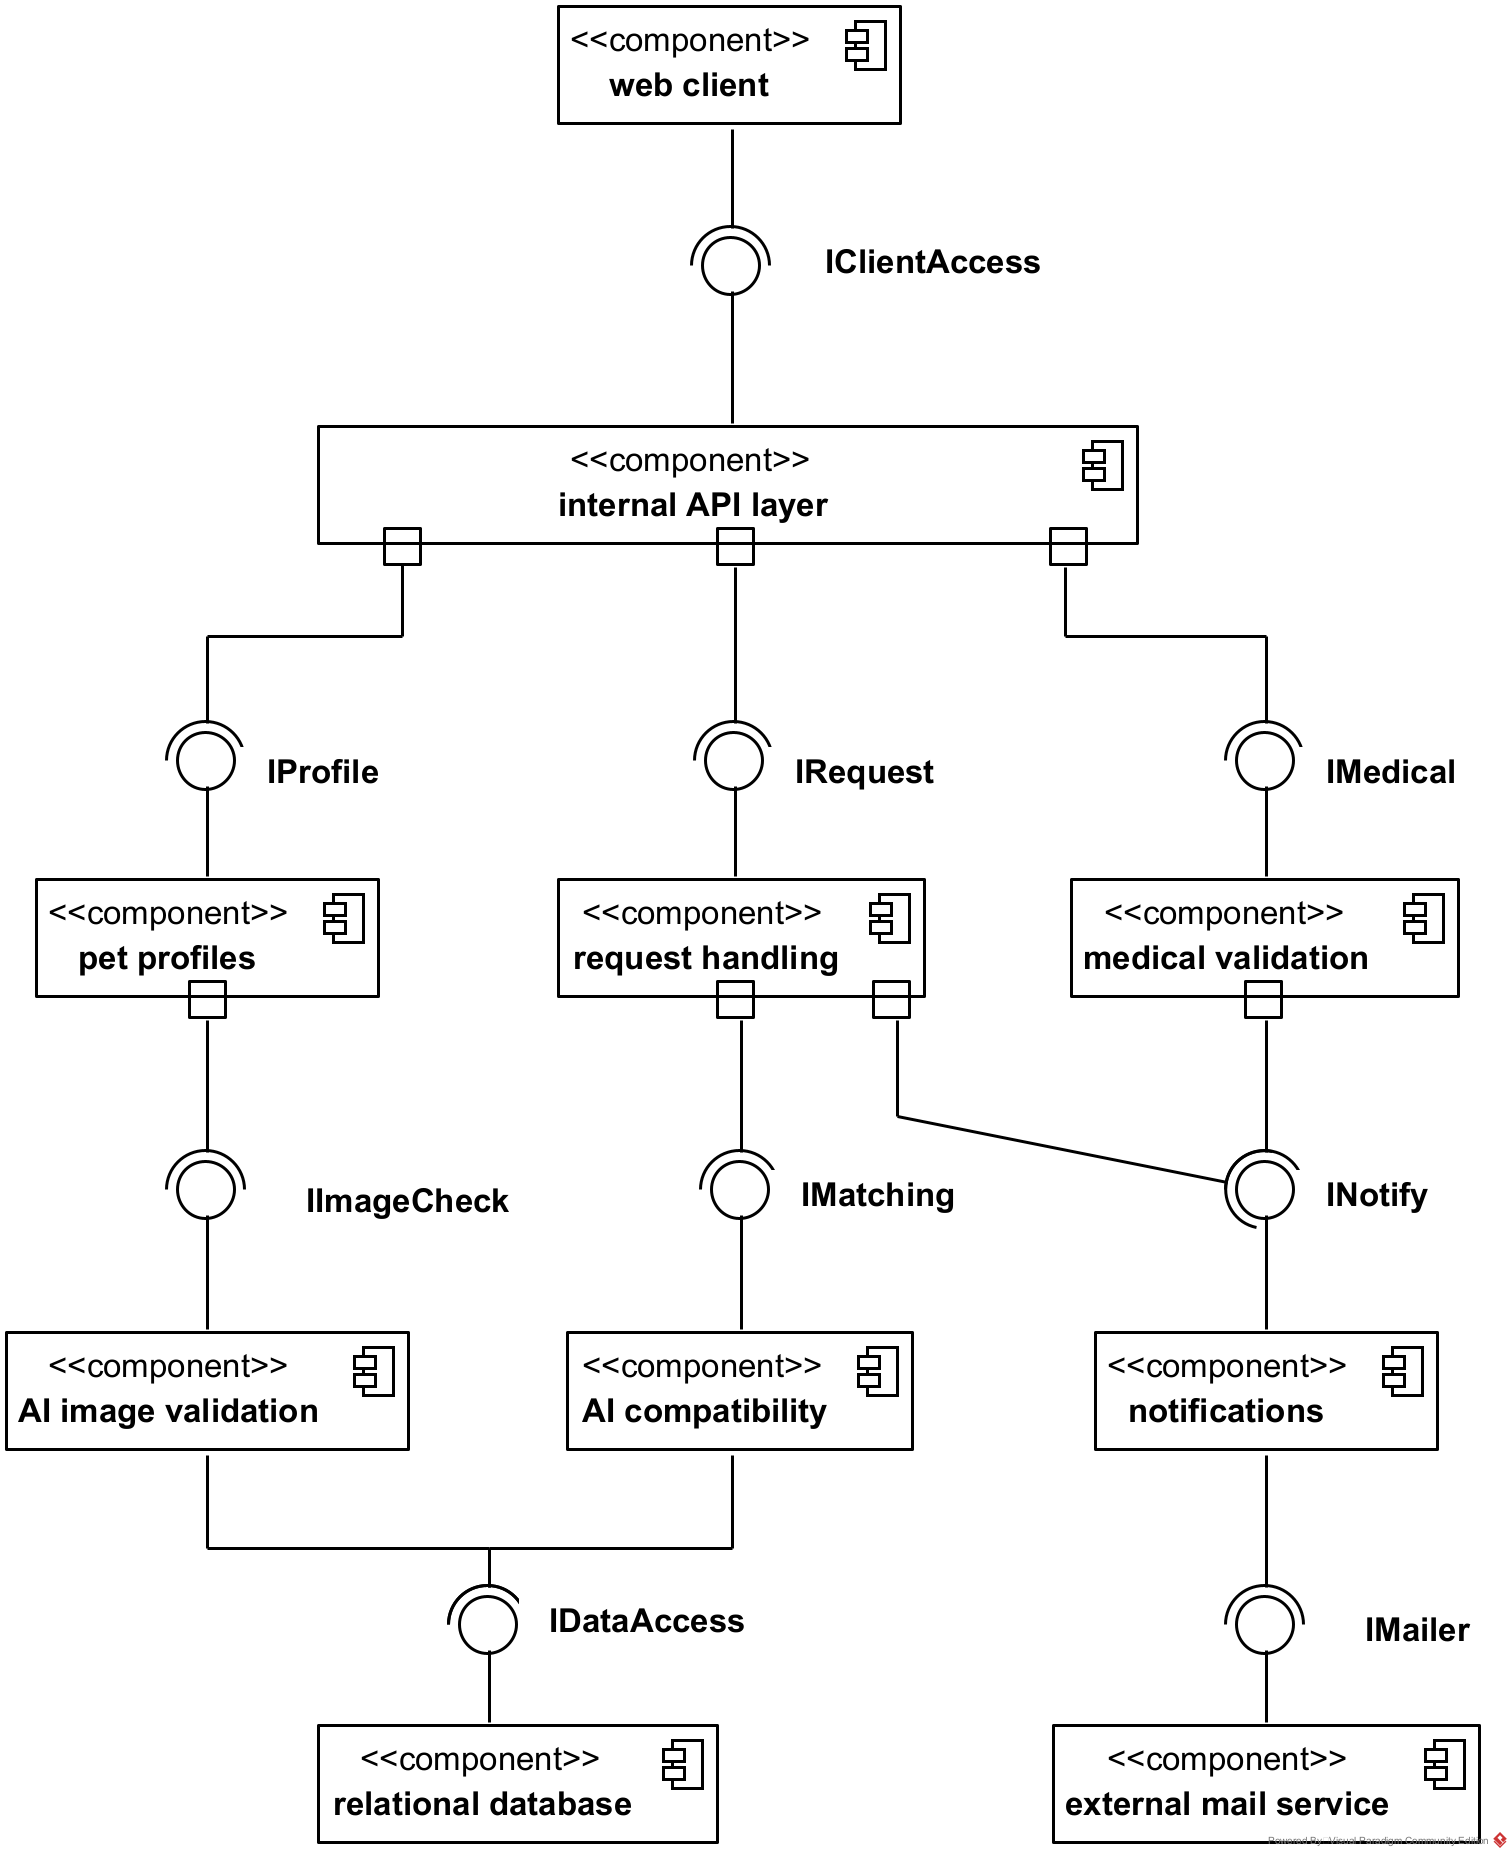
\includegraphics[width=0.75\textwidth]{DiagramaComponentes_MundiPets.png}
		\caption{Diagrama de componentes del sistema MundiPets.}
		\label{fig:componentes}
	\end{figure}
	
	La Figura~\ref{fig:componentes} muestra que la separación entre ``AI
	image validation'' y ``AI compatibility'' como componentes independientes
	que exponen sus propias interfaces (\textit{IImageCheck}, \textit{IMatching})
	hacia ``request handling'' y ``pet profiles'', en lugar de integrarse
	directamente en la lógica de negocio, refleja la decisión de aislar los
	modelos de IA del resto del sistema para poder reemplazarlos, reentrenarlos
	o degradarlos (\textit{fallback}) sin tocar la capa de API. Además, que
	``IRequest'' comparta la interfaz ``INotify'' con ``notifications'' (en
	vez de que cada componente notifique por su cuenta) muestra que las
	notificaciones se centralizaron como un servicio transversal y no como
	lógica duplicada en cada módulo.
	
	% ------------------------------------------------------------
	\subsection{Diagrama de Despliegue}
	
	\begin{figure}[H]
		\centering
		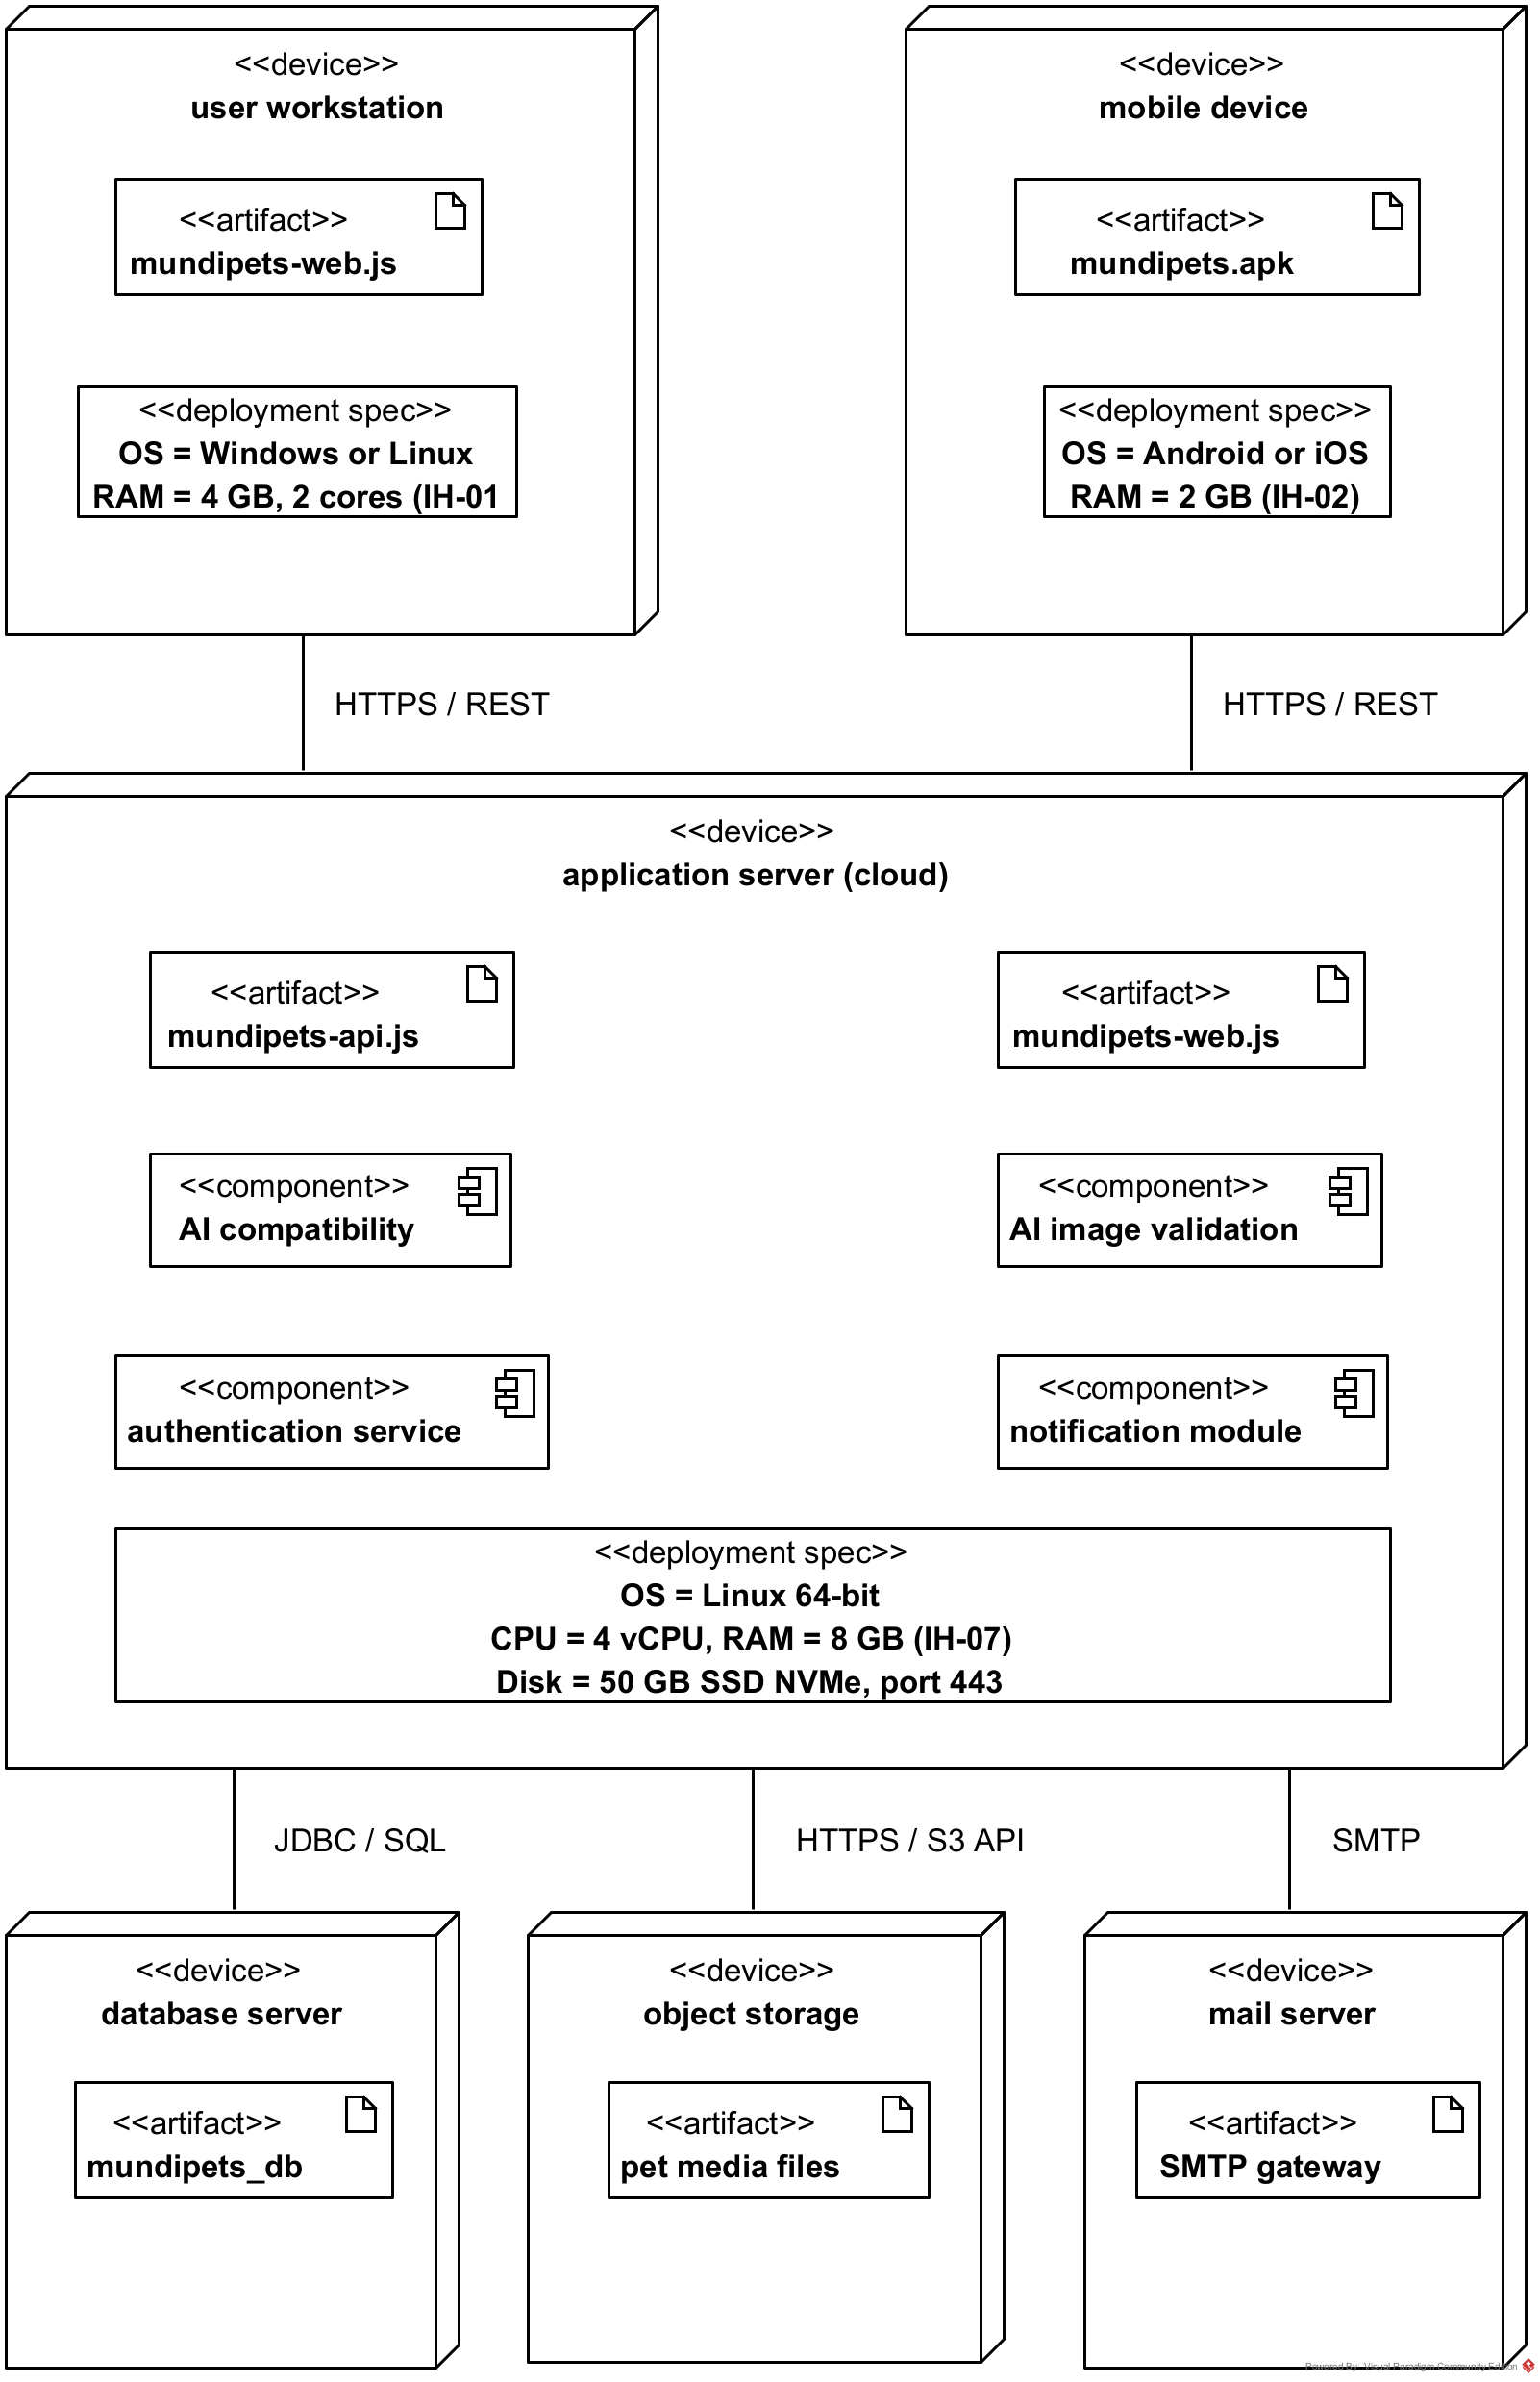
\includegraphics[width=0.8\textwidth]{DiagramaDespliegue_MundiPets.png}
		\caption{Diagrama de despliegue del sistema MundiPets.}
		\label{fig:despliegue}
	\end{figure}
	
	Que los componentes ``AI compatibility'' y ``AI image validation'' se
	desplieguen dentro del mismo nodo ``application server (cloud)'' junto con
	la autenticación y las notificaciones (y no en un nodo de cómputo dedicado
	o servicio externo separado), como se aprecia en la Figura~\ref{fig:despliegue},
	refleja que el equipo optó por una arquitectura monolítica de despliegue
	para el MVP, priorizando simplicidad operativa sobre escalabilidad
	independiente de la IA, decisión coherente con el nivel de riesgo y
	volumen de datos que maneja MundiPets en esta etapa.
	
	% ------------------------------------------------------------
	\subsection{Diagramas Estratégicos (i*)}
	
	\begin{figure}[H]
		\centering
		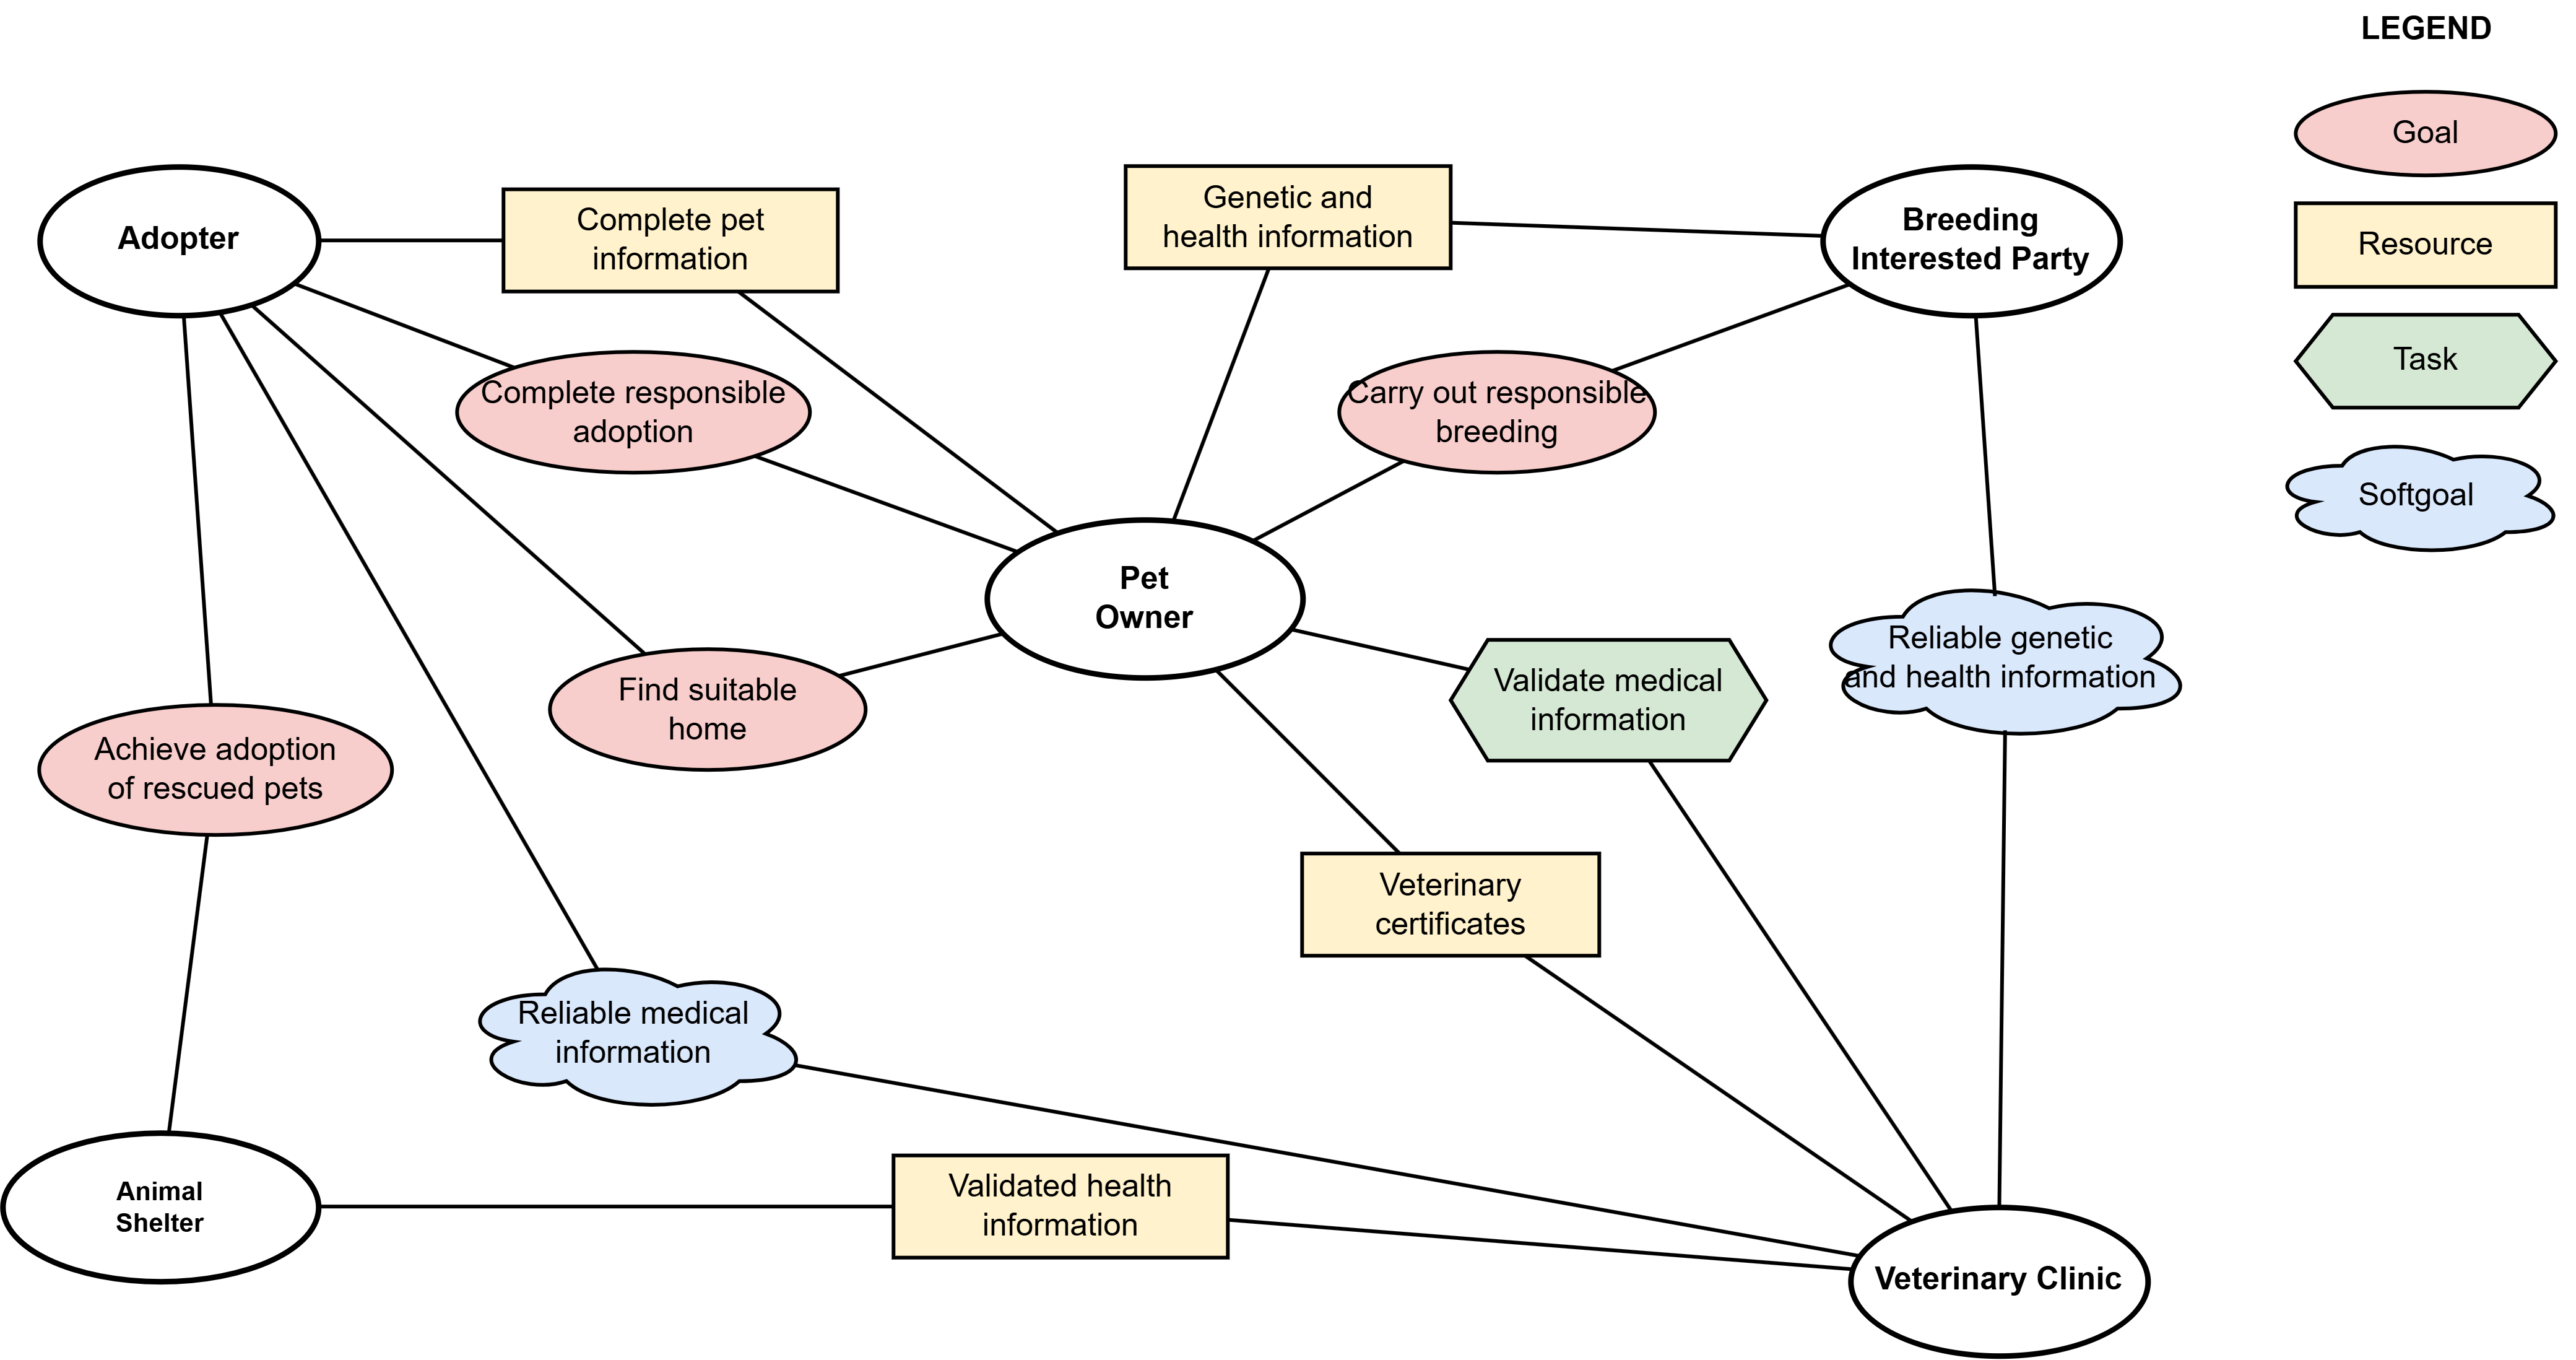
\includegraphics[width=0.95\textwidth]{DiagramaDeDependenciaEstrategica_MundiPets.png}
		\caption{Diagrama de dependencia estratégica (SD) del sistema MundiPets.}
		\label{fig:sd}
	\end{figure}
	
	En la Figura~\ref{fig:sd}, que ``Pet Owner'' dependa de ``Veterinary
	Clinic'' para la tarea ``Validate medical information'' (una tarea, no un
	simple recurso) revela que la validación médica no es un intercambio de
	datos pasivo, sino un proceso activo que el dueño no puede realizar por sí
	mismo ni delegar a otro actor: la clínica es la única fuente legítima de
	verificación, lo que justifica por qué el ERS exige trazabilidad hacia un
	actor externo verificador y no solo un campo de texto autodeclarado.
	
	\begin{figure}[H]
		\centering
		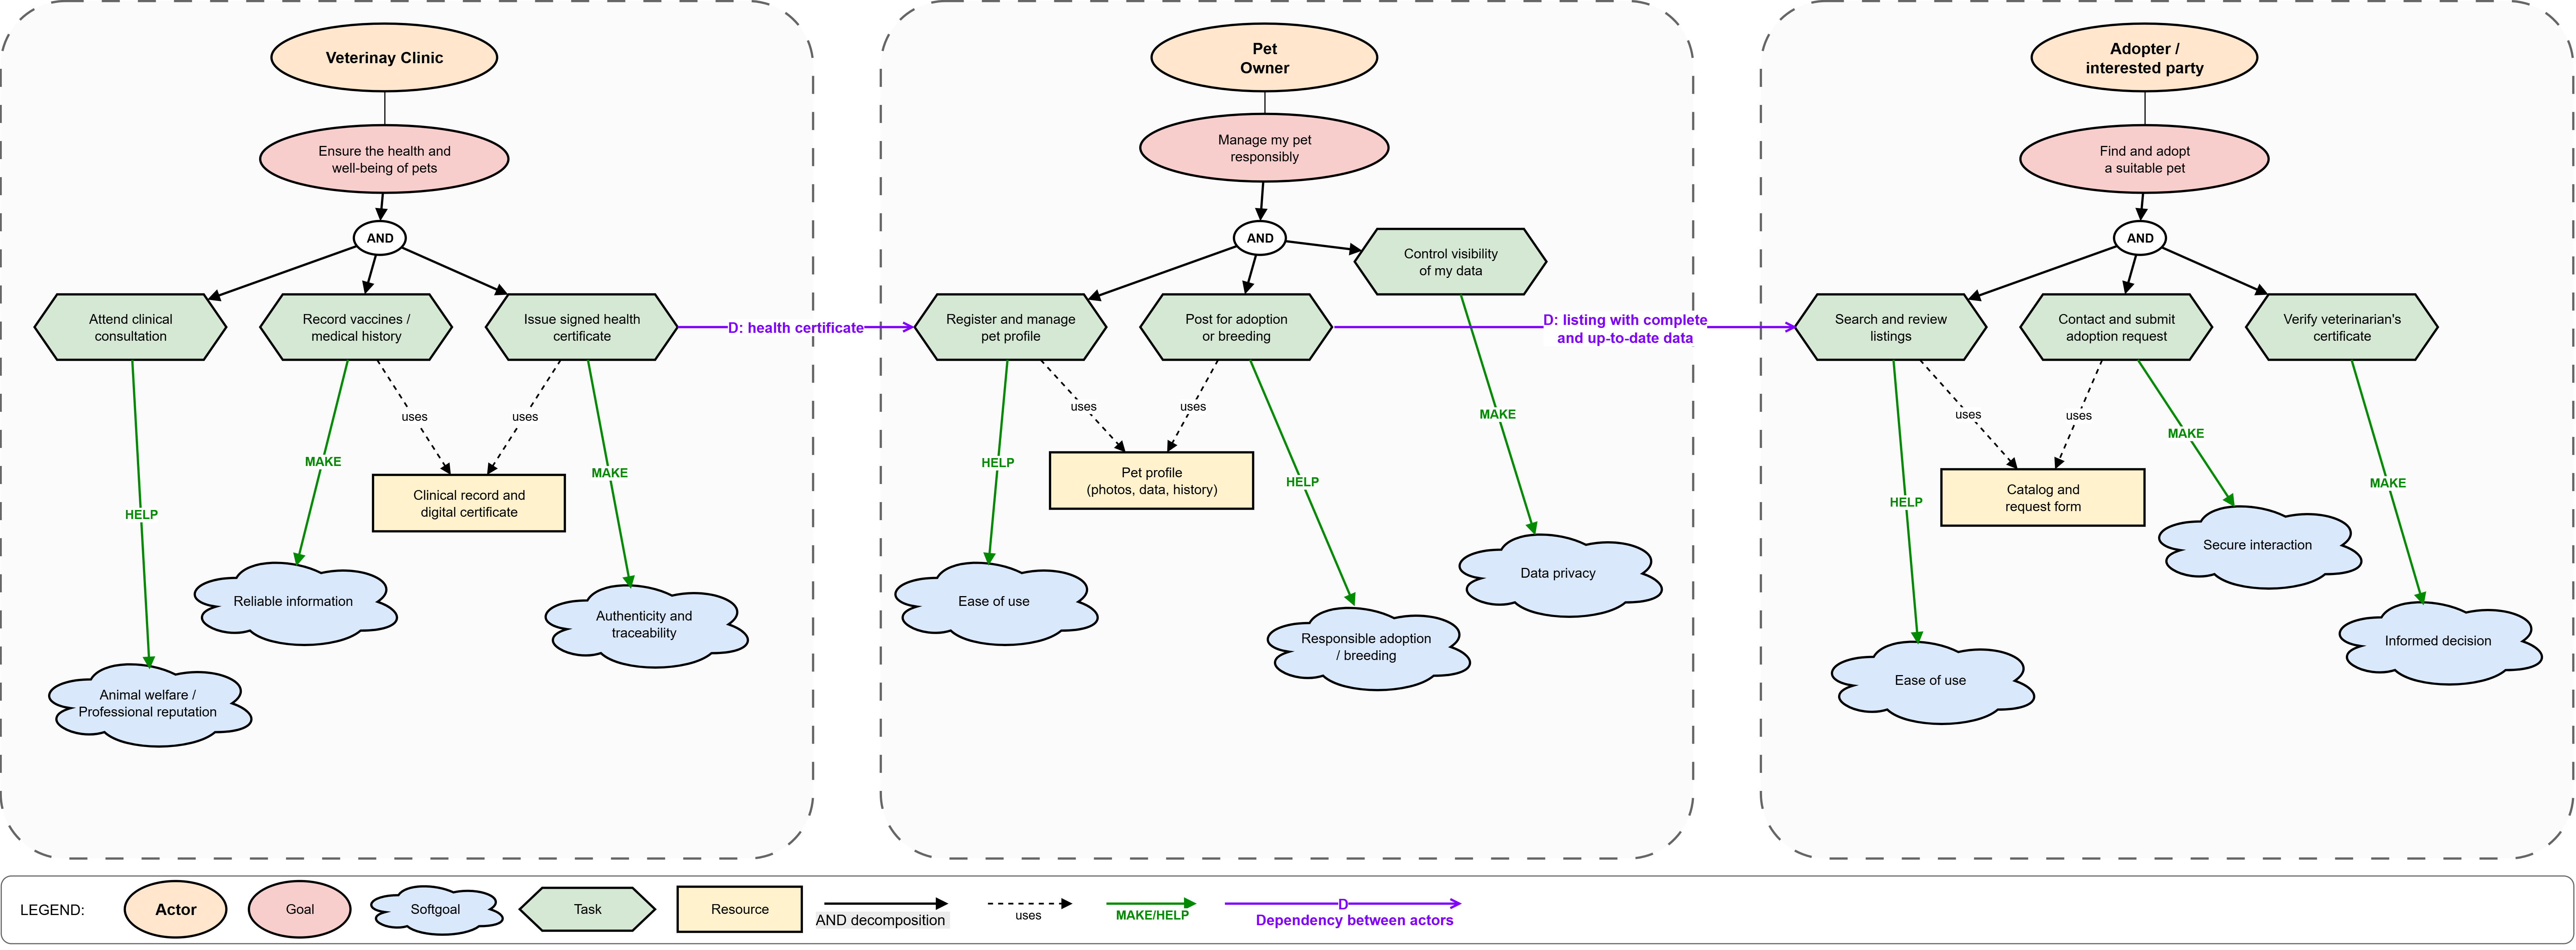
\includegraphics[width=0.95\textwidth]{DiagramaDeRazonEstrategica_MundiPets.png}
		\caption{Diagrama de razón estratégica (SR) del sistema MundiPets.}
		\label{fig:sr}
	\end{figure}
	
	Dentro del racional del ``Pet Owner'' en la Figura~\ref{fig:sr}, que
	``Post for adoption or breeding'' dependa del recurso ``Pet profile
	(photos, data, history)'' mediante \textit{uses} (y no que ambas tareas
	generen su propio perfil por separado) refleja la decisión de que el
	perfil de la mascota es un artefacto único y compartido entre los flujos
	de adopción y de cruza, evitando duplicidad de datos y asegurando que
	cualquier corrección al perfil (por ejemplo, del historial médico) se
	propague automáticamente a ambos procesos.
	
	% ------------------------------------------------------------
	\subsection{Diagrama de Flujo de Datos (Nivel 1)}

	\begin{figure}[H]
		\centering
		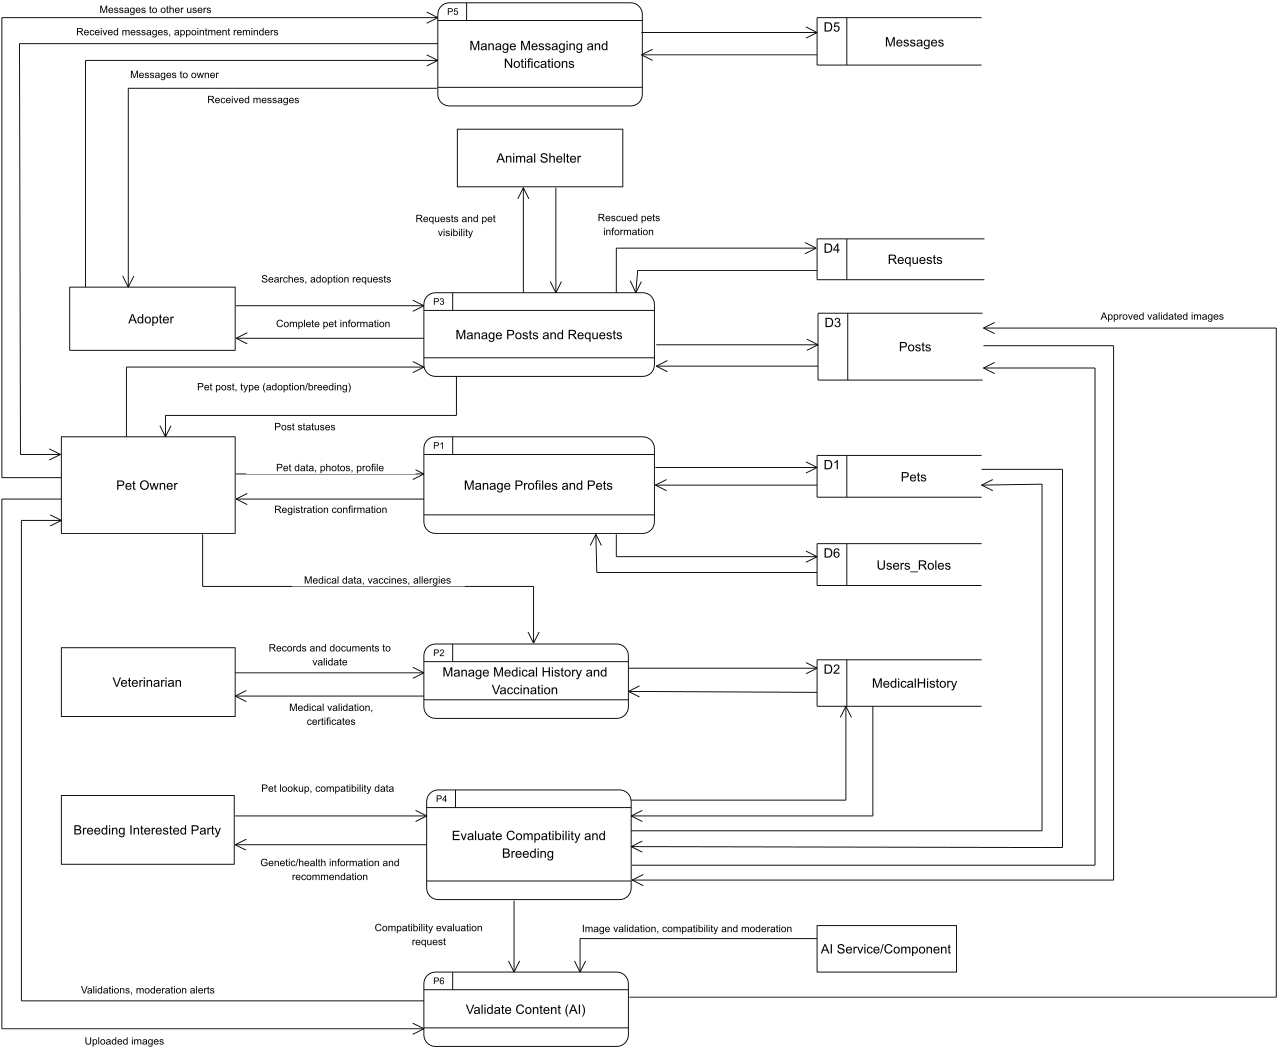
\includegraphics[width=0.95\textwidth]{Diagrama_DFD_MundiPets.png}
		\caption{Diagrama de flujo de datos, Nivel 1, notación Yourdon--DeMarco.}
		\label{fig:dfd_nivel1}
	\end{figure}

	Que el proceso único ``0. MundiPets'' del Diagrama de Contexto
	(Figura~\ref{fig:contexto}, que funciona como DFD Nivel 0) se
	descomponga en exactamente seis procesos (P1 Manage Profiles and Pets,
	P2 Manage Medical History and Vaccination, P3 Manage Posts and
	Requests, P4 Evaluate Compatibility and Breeding, P5 Manage Messaging
	and Notifications, P6 Validate Content) revela que el equipo agrupó la
	funcionalidad del sistema por dominio de datos compartido y no por
	actor o por caso de uso individual: P2, por ejemplo, concentra tanto el
	registro del historial médico (RF-02) como su validación profesional
	(RF-09) y la trazabilidad de vacunas (RF-14, RF-24), porque las tres
	operan sobre el mismo almacén D2 (MedicalHistory), aunque correspondan
	a actores distintos (propietario y veterinaria). Que P6 (``Validate
	Content'') se mantenga como proceso independiente, con su propio flujo
	de entrada y salida hacia el ``AI Service/Component'' ya visto en el
	Diagrama de Contexto, refuerza la misma decisión de aislamiento de la
	IA observada en el Diagrama de Componentes: el flujo de datos de la
	validación automática nunca se mezcla con el flujo de datos de negocio
	de los demás procesos, sino que pasa siempre por un almacén y un
	proceso propios.

	% ------------------------------------------------------------
	\subsection{Diagramas de Máquinas de Estado}
	
	\begin{figure}[H]
		\centering
		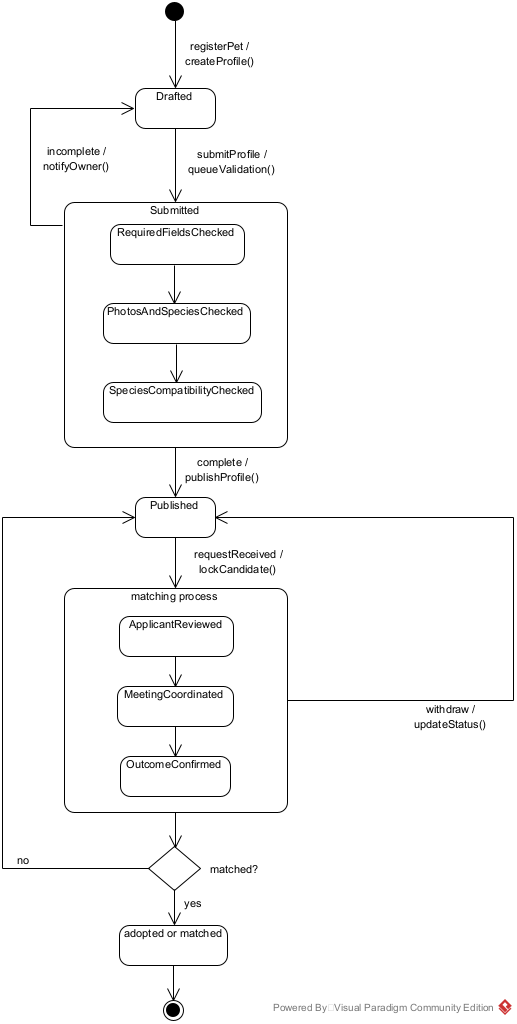
\includegraphics[width=0.55\textwidth]{DiagramaMaquinasEstado_PerfilMascota_MundiPets.png}
		\caption{Diagrama de máquinas de estado -- Perfil Mascota.}
		\label{fig:me_perfil}
	\end{figure}
	
	Que el estado ``Submitted'' sea un subestado compuesto con una secuencia
	interna obligatoria (\textit{RequiredFieldsChecked} $\rightarrow$
	\textit{PhotosAndSpeciesChecked} $\rightarrow$
	\textit{SpeciesCompatibilityChecked}) antes de poder llegar a
	``Published'', como se ve en la Figura~\ref{fig:me_perfil}, revela que la
	publicación de una mascota nunca es un evento atómico, sino el resultado
	de una validación en capas donde ningún criterio puede saltarse: si falta
	un campo, el sistema regresa a ``Drafted'' y notifica al dueño en vez de
	dejar el perfil a medio camino. Asimismo, que ``matched?'' sea una
	decisión posterior a todo el subestado ``matching process'' (y no una
	simple bandera booleana temprana) muestra que el sistema exige agotar la
	revisión del solicitante, coordinación de encuentro y confirmación del
	resultado antes de decidir si hubo adopción o cruza exitosa, evitando
	cierres prematuros del caso.
	
	\begin{figure}[H]
		\centering
		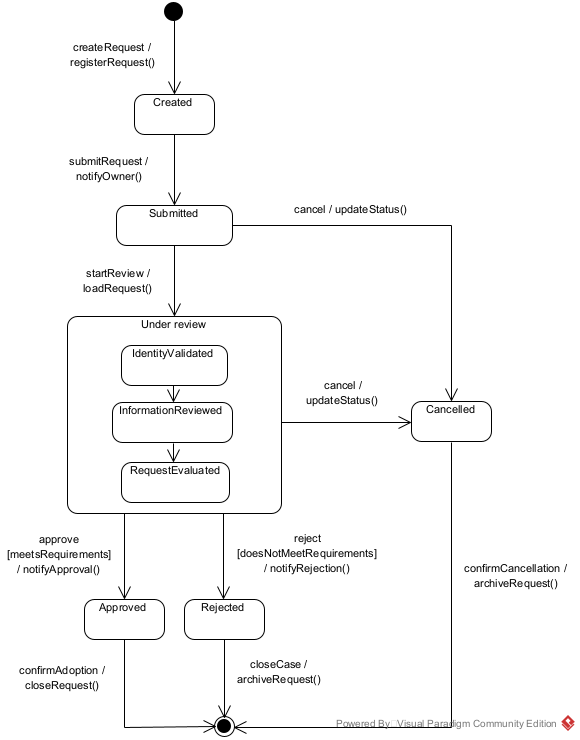
\includegraphics[width=0.6\textwidth]{DiagramaMaquinasEstado_Solicitudes_MundiPets.png}
		\caption{Diagrama de máquinas de estado -- Solicitudes.}
		\label{fig:me_solicitudes}
	\end{figure}
	
	Que ``cancel'' esté habilitado tanto desde ``Submitted'' como desde
	dentro de ``Under review'' (dos transiciones distintas hacia
	``Cancelled'', no una sola desde el estado padre), tal como se muestra en
	la Figura~\ref{fig:me_solicitudes}, refleja que el diseño reconoce que
	una solicitud puede ser retirada por el interesado en cualquier punto del
	proceso, incluso mientras ya se está validando la identidad o evaluando
	la solicitud, y no únicamente antes de empezar la revisión. Además, que
	``Approved'' y ``Rejected'' conduzcan a acciones finales distintas
	(\textit{confirmAdoption} vs.\ \textit{closeCase}, ambas con
	\textit{archiveRequest()}) en lugar de una única salida genérica, indica
	que el cierre de una adopción concretada exige un paso adicional de
	confirmación que el cierre de un rechazo no necesita, correspondiendo a
	una responsabilidad distinta según el desenlace.
	
	\begin{figure}[H]
		\centering
		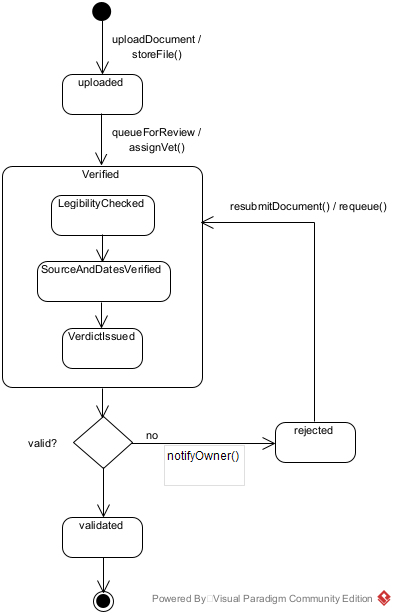
\includegraphics[width=0.5\textwidth]{DiagramaMaquinasEstado_VerificacionDocumentos_MundiPets.png}
		\caption{Diagrama de máquinas de estado -- Verificación de Documentos.}
		\label{fig:me_verificacion}
	\end{figure}
	
	Que \textit{resubmitDocument()/requeue()} regrese exclusivamente desde
	``rejected'' hacia el subestado compuesto ``Verified'' (y no hacia
	``uploaded''), como se aprecia en la Figura~\ref{fig:me_verificacion},
	revela que un documento rechazado no reinicia el ciclo completo de carga,
	sino que retorna directamente a la cola de revisión una vez corregido,
	evitando que el dueño tenga que subir el archivo desde cero. También, que
	la verificación interna se descomponga en tres pasos secuenciales
	(legibilidad $\rightarrow$ verificación de fuente y fechas
	$\rightarrow$ emisión de veredicto) antes de la decisión ``valid?''
	muestra que el sistema separa expresamente la validez formal del
	documento (que se lea bien) de su validez de contenido (que la fuente y
	fechas sean correctas), permitiendo auditar en qué paso específico falló
	un documento rechazado.
	
	% ------------------------------------------------------------
	\subsection{Diagramas de Secuencia}
	
	\subsubsection{Registrar mascota (CU-01)}
	
	\begin{figure}[H]
		\centering
		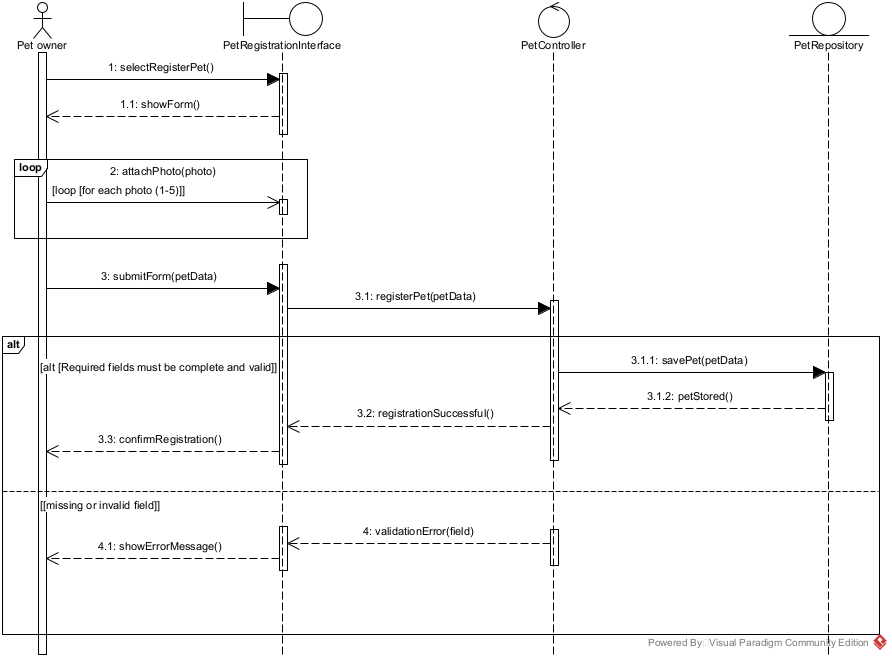
\includegraphics[width=0.95\textwidth]{DiagramaSecuencia_CU-01_MundiPets.png}
		\caption{Diagrama de secuencia -- Registrar mascota (CU-01).}
		\label{fig:sec_cu01}
	\end{figure}
	
	En la Figura~\ref{fig:sec_cu01}, que \textit{attachPhoto(photo)} se
	ejecute en un \textit{loop} previo al \textit{submitForm(petData)} (y no
	como parte del mismo envío) revela que el diseño separa la carga
	incremental de fotos de la validación final del formulario, permitiendo
	que el dueño adjunte entre 1 y 5 fotos de forma progresiva antes de
	comprometerse a enviar el registro completo. Además, que la validación de
	campos ocurra en el \textit{PetController} y no en la interfaz (el
	\textit{alt} evalúa ``Required fields must be complete and valid'' a
	nivel de controlador) muestra que la lógica de negocio, no la capa de
	presentación, es la responsable de decidir si el registro es válido.
	
	\subsubsection{Registrar historial médico y antecedentes genéticos (CU-02)}
	
	\begin{figure}[H]
		\centering
		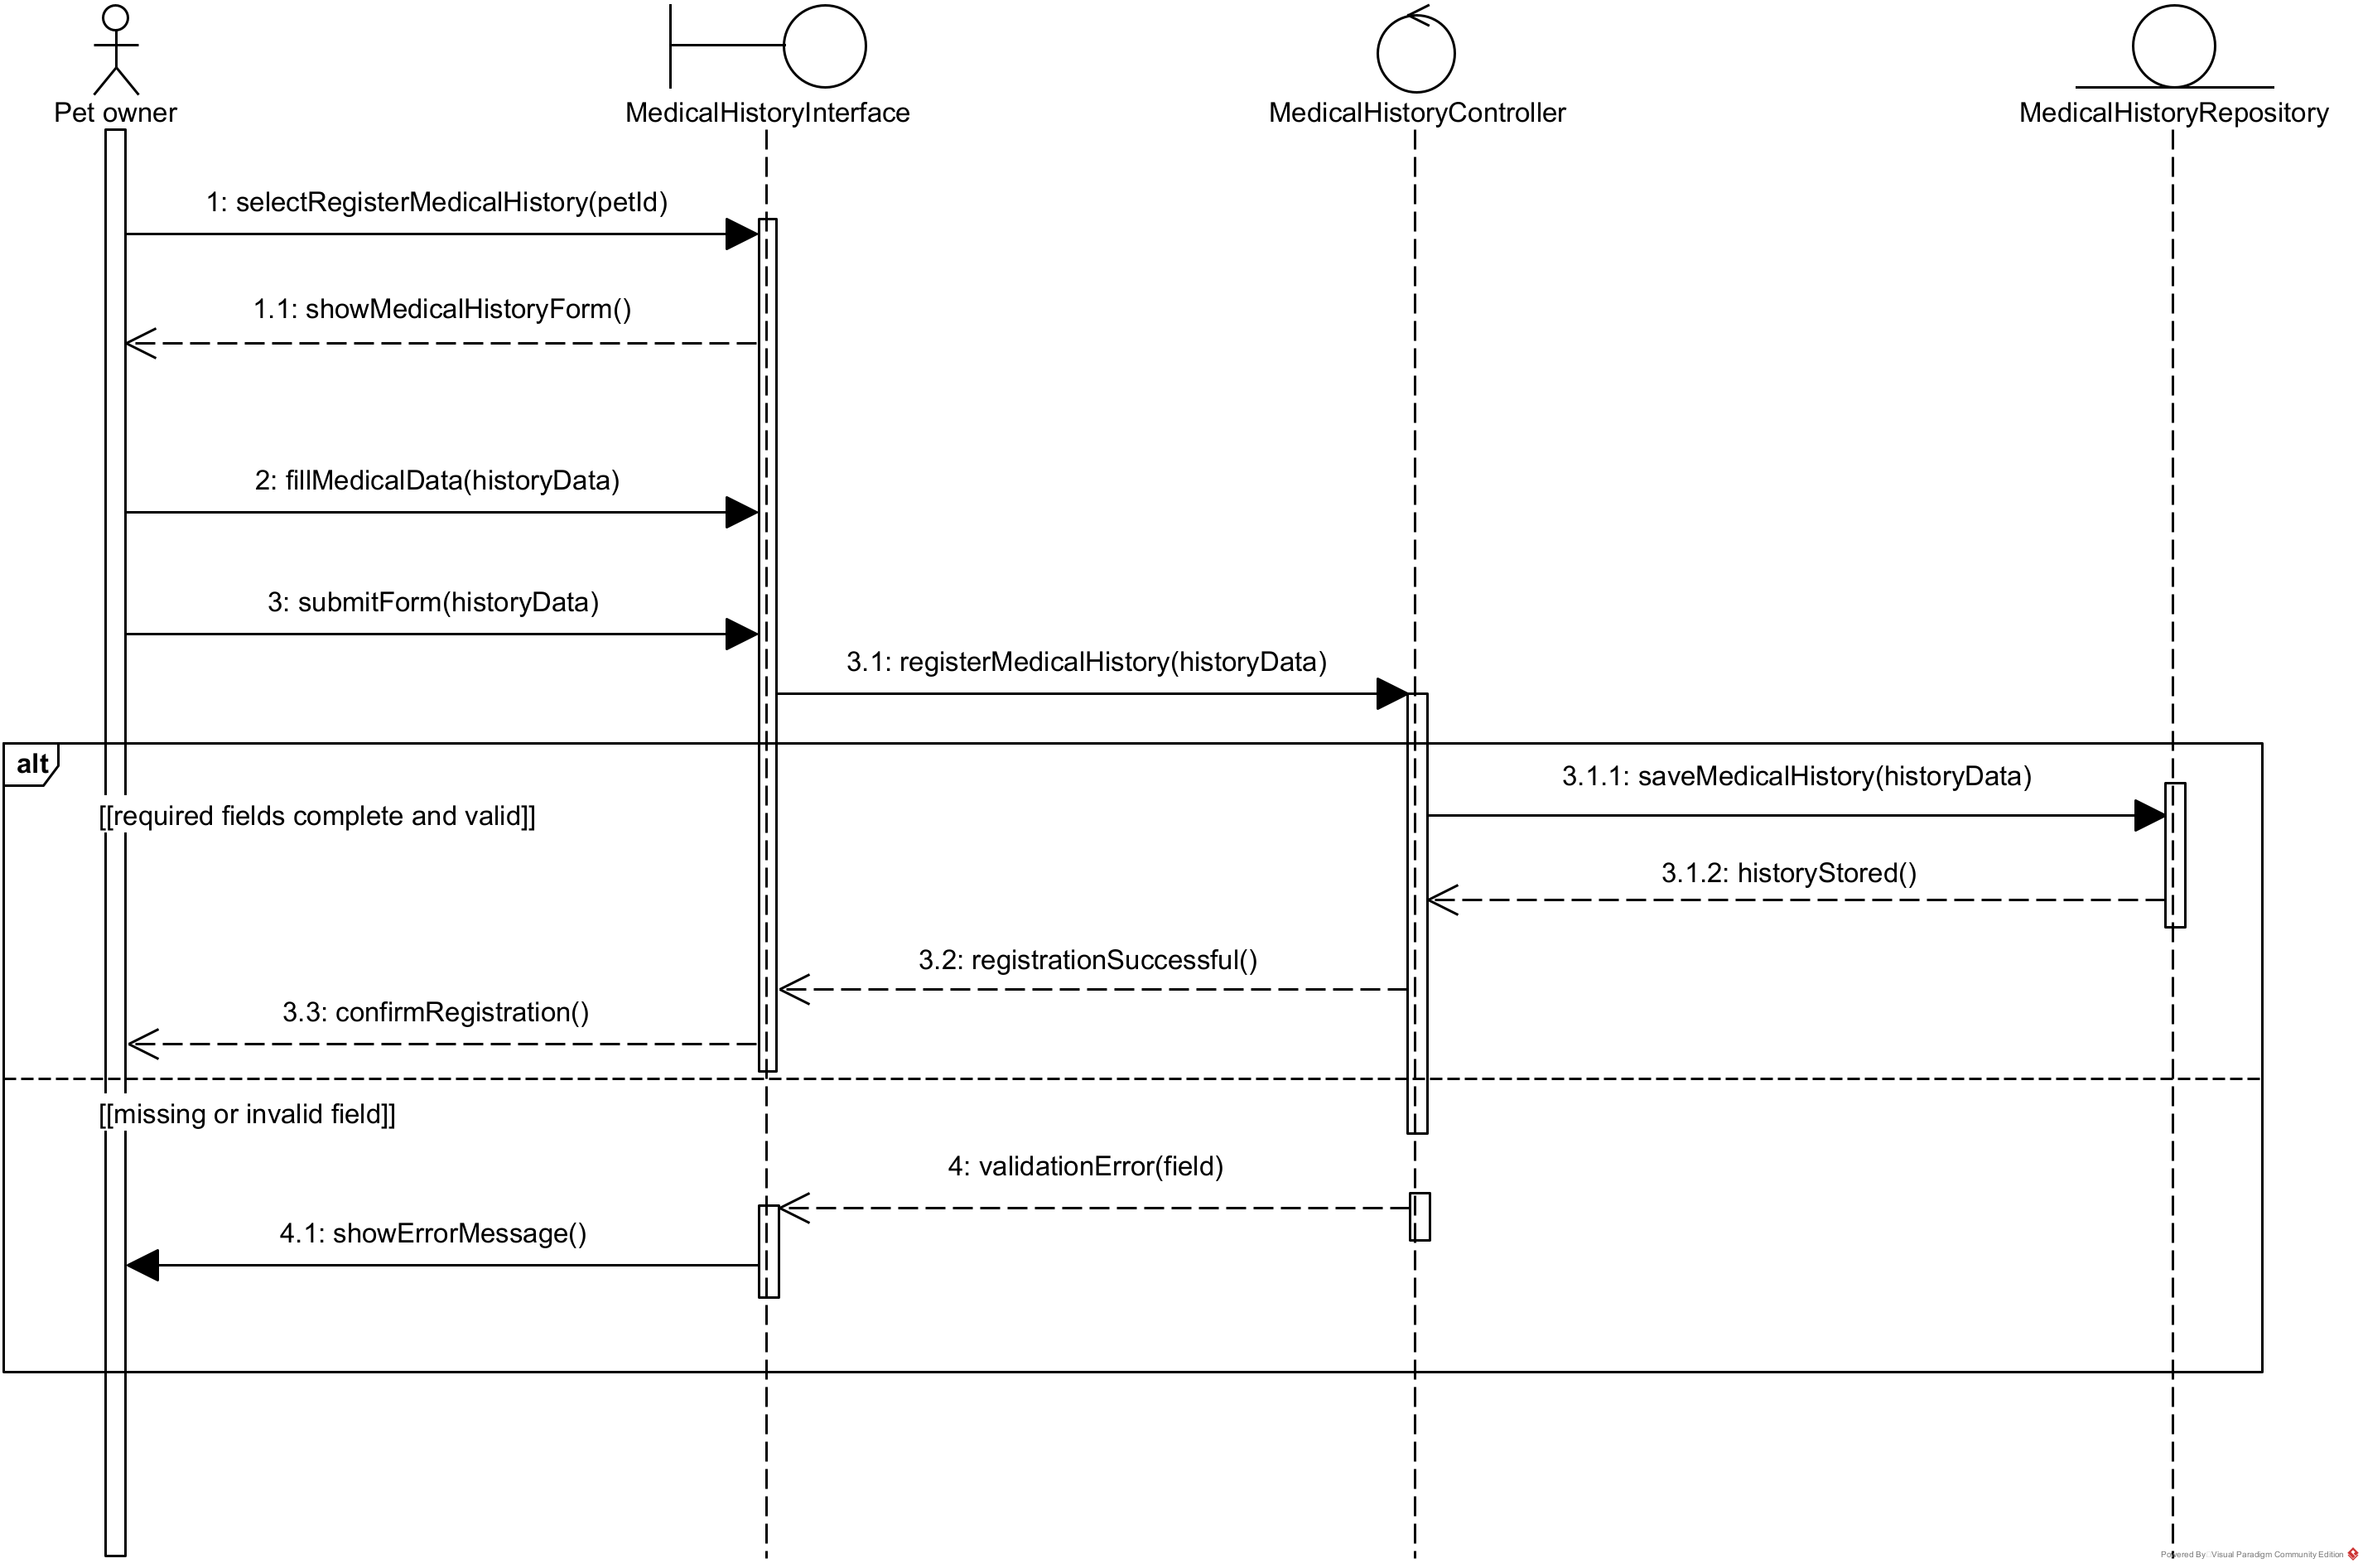
\includegraphics[width=0.9\textwidth]{DiagramaSecuencia_CU-02_MundiPets.png}
		\caption{Diagrama de secuencia -- Registrar historial médico y antecedentes genéticos (CU-02).}
		\label{fig:sec_cu02}
	\end{figure}
	
	La estructura casi idéntica al CU-01 (mismo patrón de \textit{alt} con
	validación en el controlador), visible en la Figura~\ref{fig:sec_cu02},
	refleja una decisión consciente de reutilizar el mismo patrón
	arquitectónico de registro para todo dato del sistema, de forma que el
	equipo pueda mantener consistencia entre módulos distintos (mascota vs.\
	historial médico) sin duplicar convenciones. Esto evidencia que el
	historial médico se trata como una entidad de registro independiente y no
	como un campo más del perfil de la mascota.
	
	\subsubsection{Cargar documento veterinario y carnet de vacunación (CU-03)}
	
	\begin{figure}[H]
		\centering
		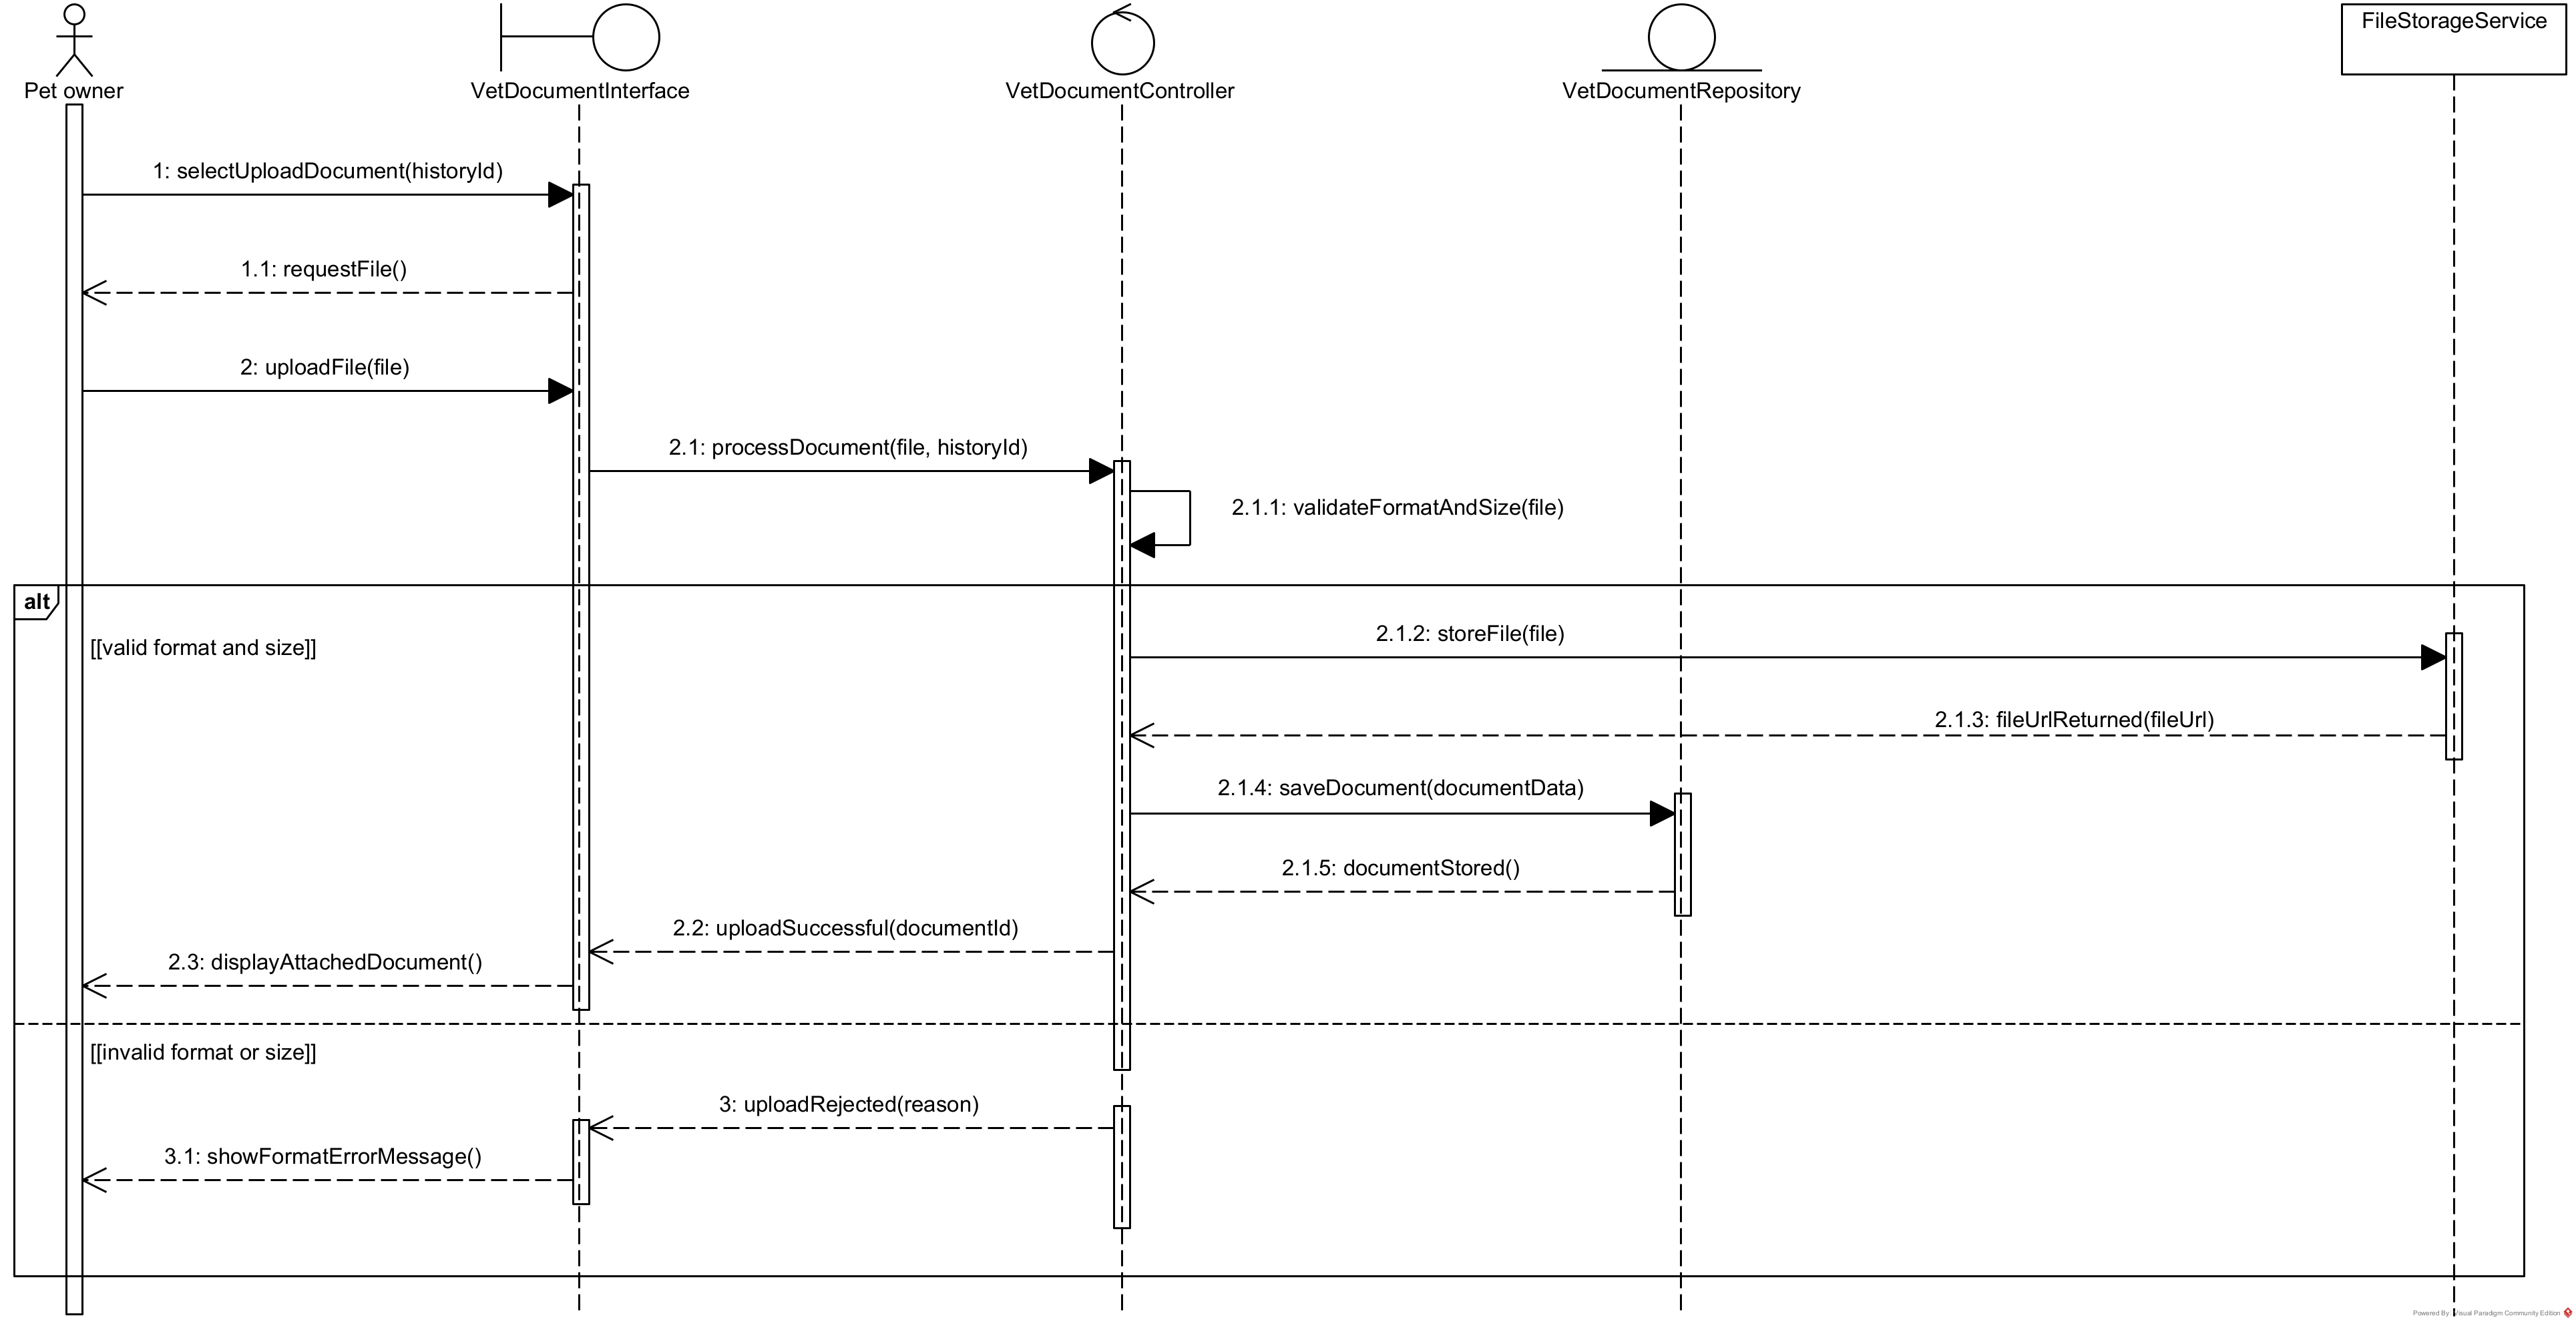
\includegraphics[width=0.95\textwidth]{DiagramaSecuencia_CU-03_MundiPets.png}
		\caption{Diagrama de secuencia -- Cargar documento veterinario y carnet de vacunación (CU-03).}
		\label{fig:sec_cu03}
	\end{figure}
	
	Que \textit{validateFormatAndSize(file)} sea una llamada reflexiva del
	propio \textit{VetDocumentController} (mensaje a sí mismo) antes de
	invocar al \textit{FileStorageService}, como se ve en la
	Figura~\ref{fig:sec_cu03}, revela que el sistema nunca envía un archivo a
	almacenamiento externo sin antes garantizar localmente que cumple formato
	y tamaño, evitando cargas costosas o inseguras a un servicio de terceros.
	También, que \textit{storeFile} preceda a \textit{saveDocument} (primero
	el archivo físico, luego el registro en base de datos) muestra que el
	diseño prioriza tener la evidencia física respaldada antes de dejar
	constancia lógica de que el documento existe.
	
	\subsubsection{Publicar mascota en adopción (CU-04)}
	
	\begin{figure}[H]
		\centering
		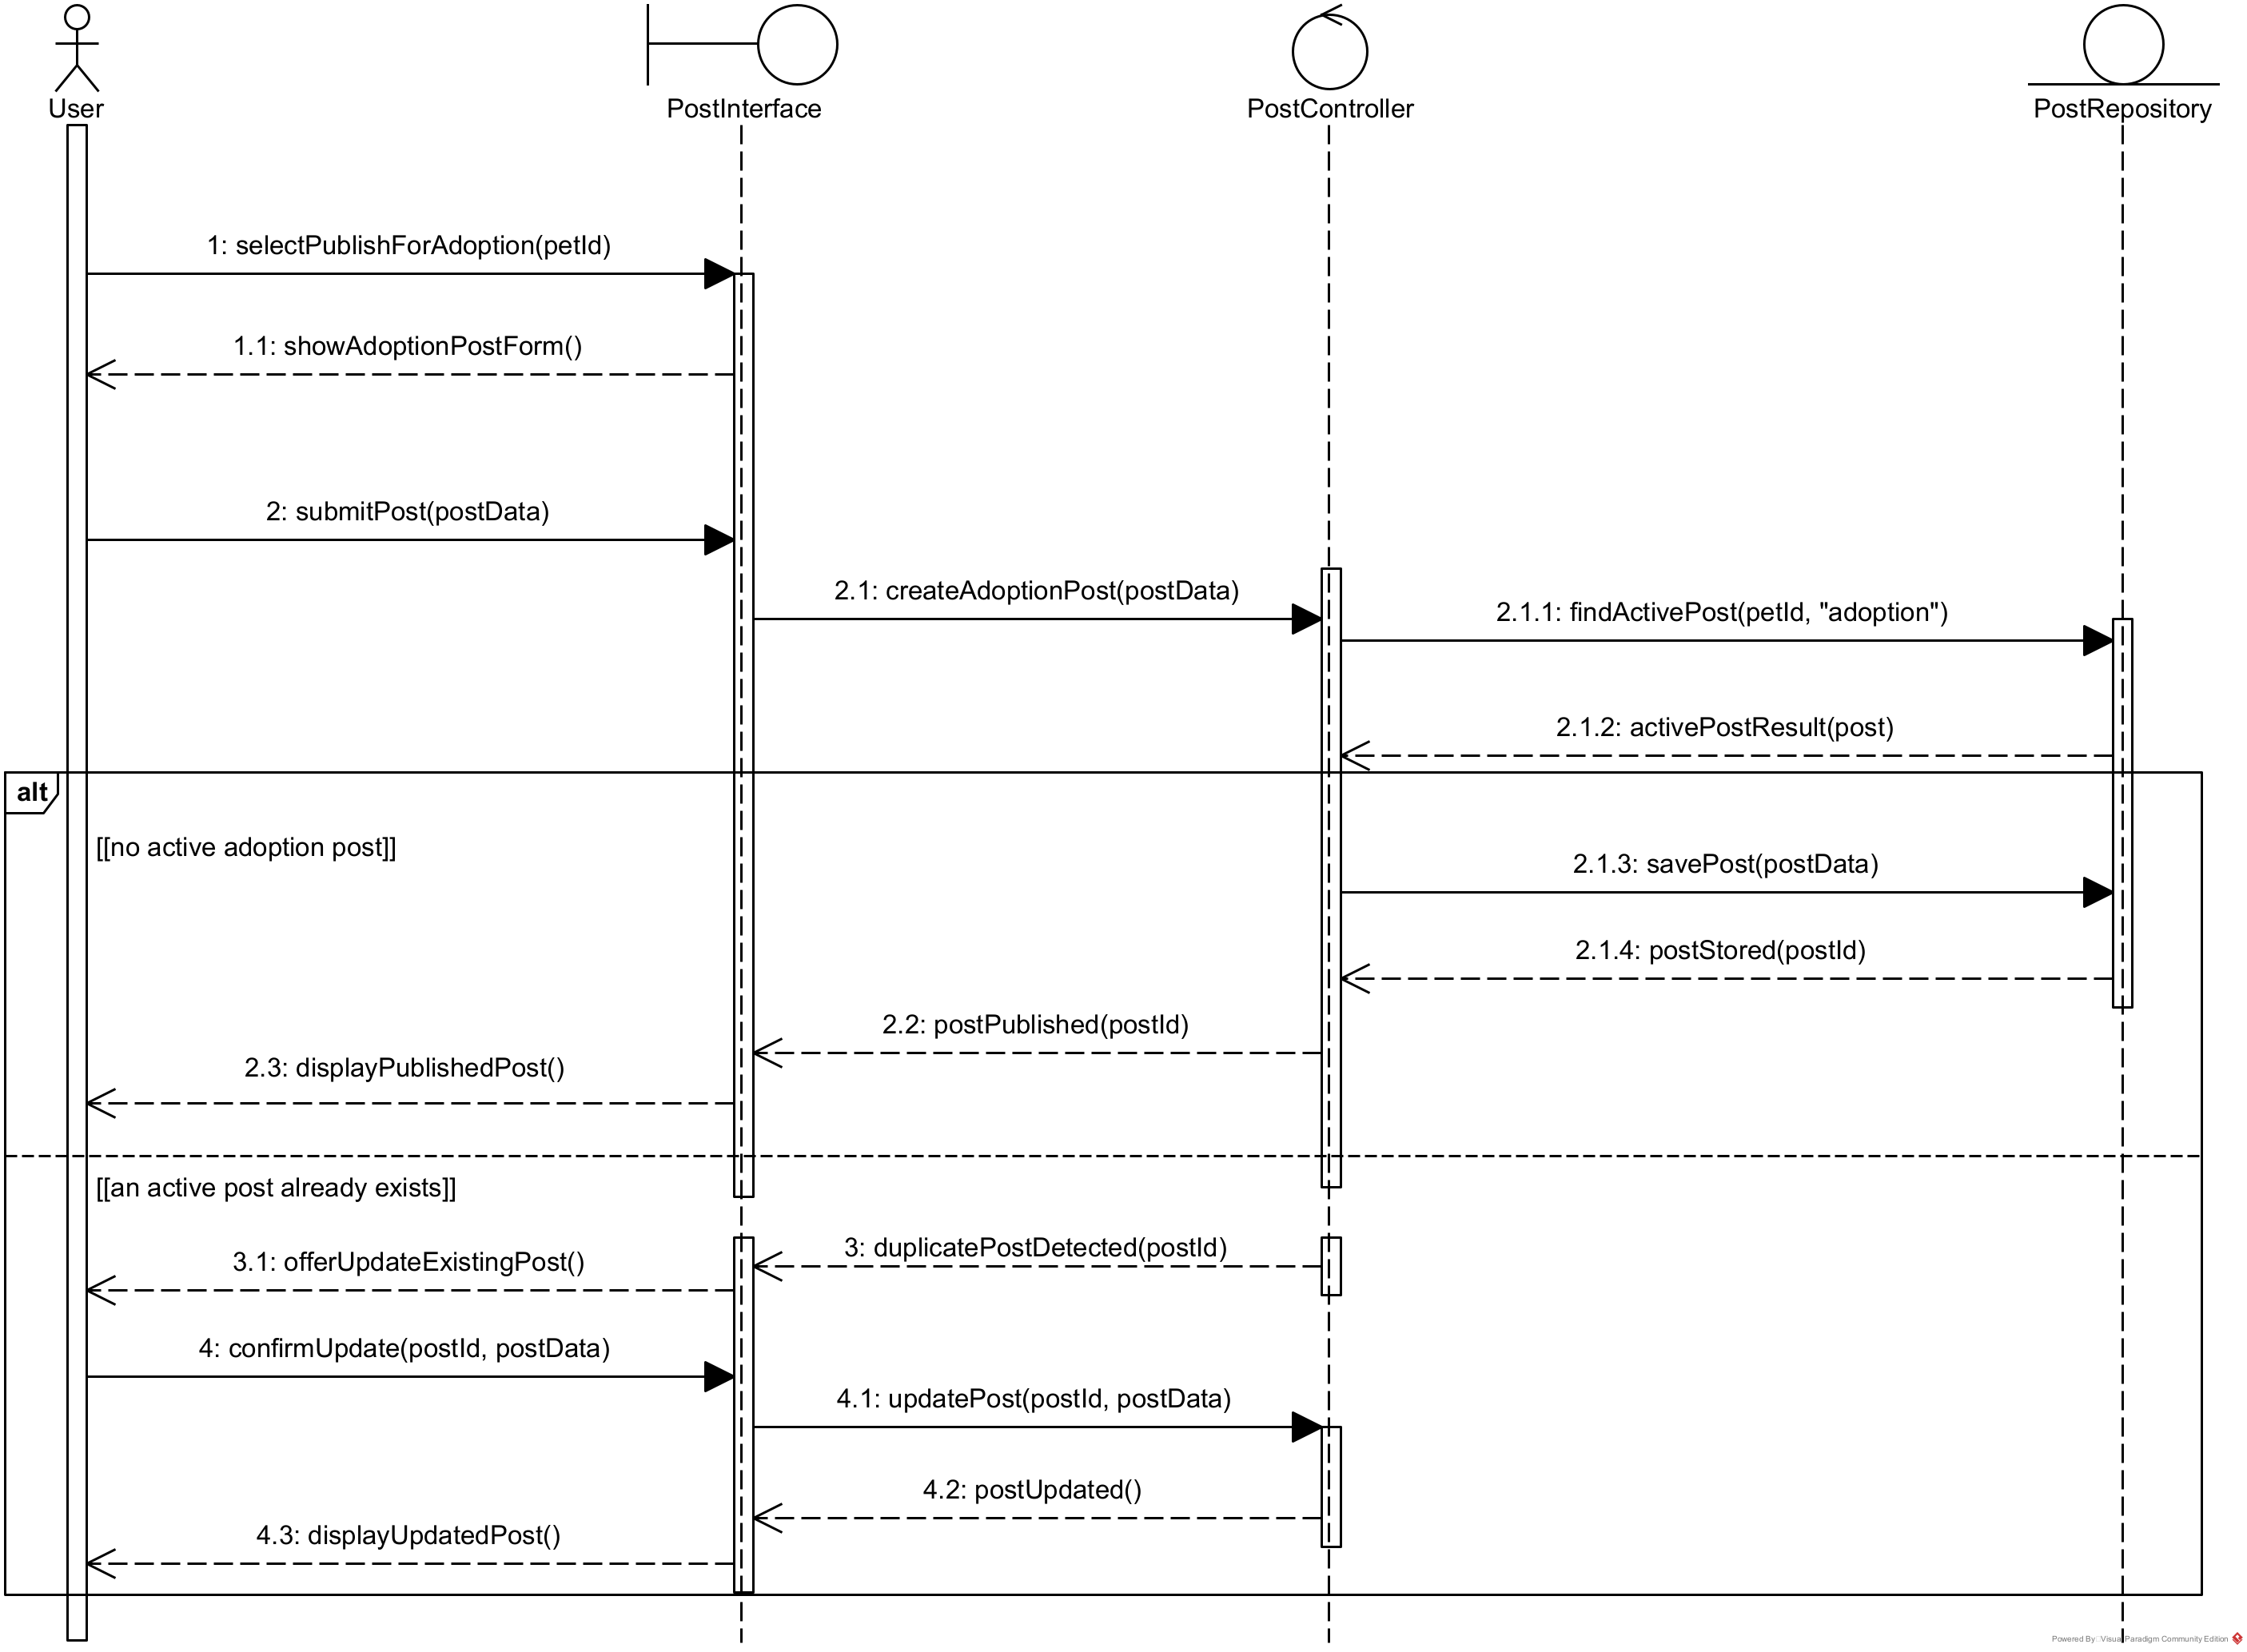
\includegraphics[width=0.95\textwidth]{DiagramaSecuencia_CU-04_MundiPets.png}
		\caption{Diagrama de secuencia -- Publicar mascota en adopción (CU-04).}
		\label{fig:sec_cu04}
	\end{figure}
	
	La verificación \textit{findActivePost(petId, "adoption")} antes de
	decidir entre crear o actualizar, presente en la Figura~\ref{fig:sec_cu04},
	revela que el sistema previene activamente publicaciones duplicadas de
	una misma mascota, tratando la unicidad de la publicación activa como una
	regla de negocio explícita y no como una validación de interfaz. Que el
	flujo de ``an active post already exists'' ofrezca actualizar en lugar
	de simplemente rechazar el nuevo intento (\textit{offerUpdateExistingPost})
	muestra que el diseño prioriza la conveniencia del usuario sobre el
	rechazo estricto.
	
	\subsubsection{Publicar mascota para cruza y gestionar solicitud (CU-05)}
	
	\begin{figure}[H]
		\centering
		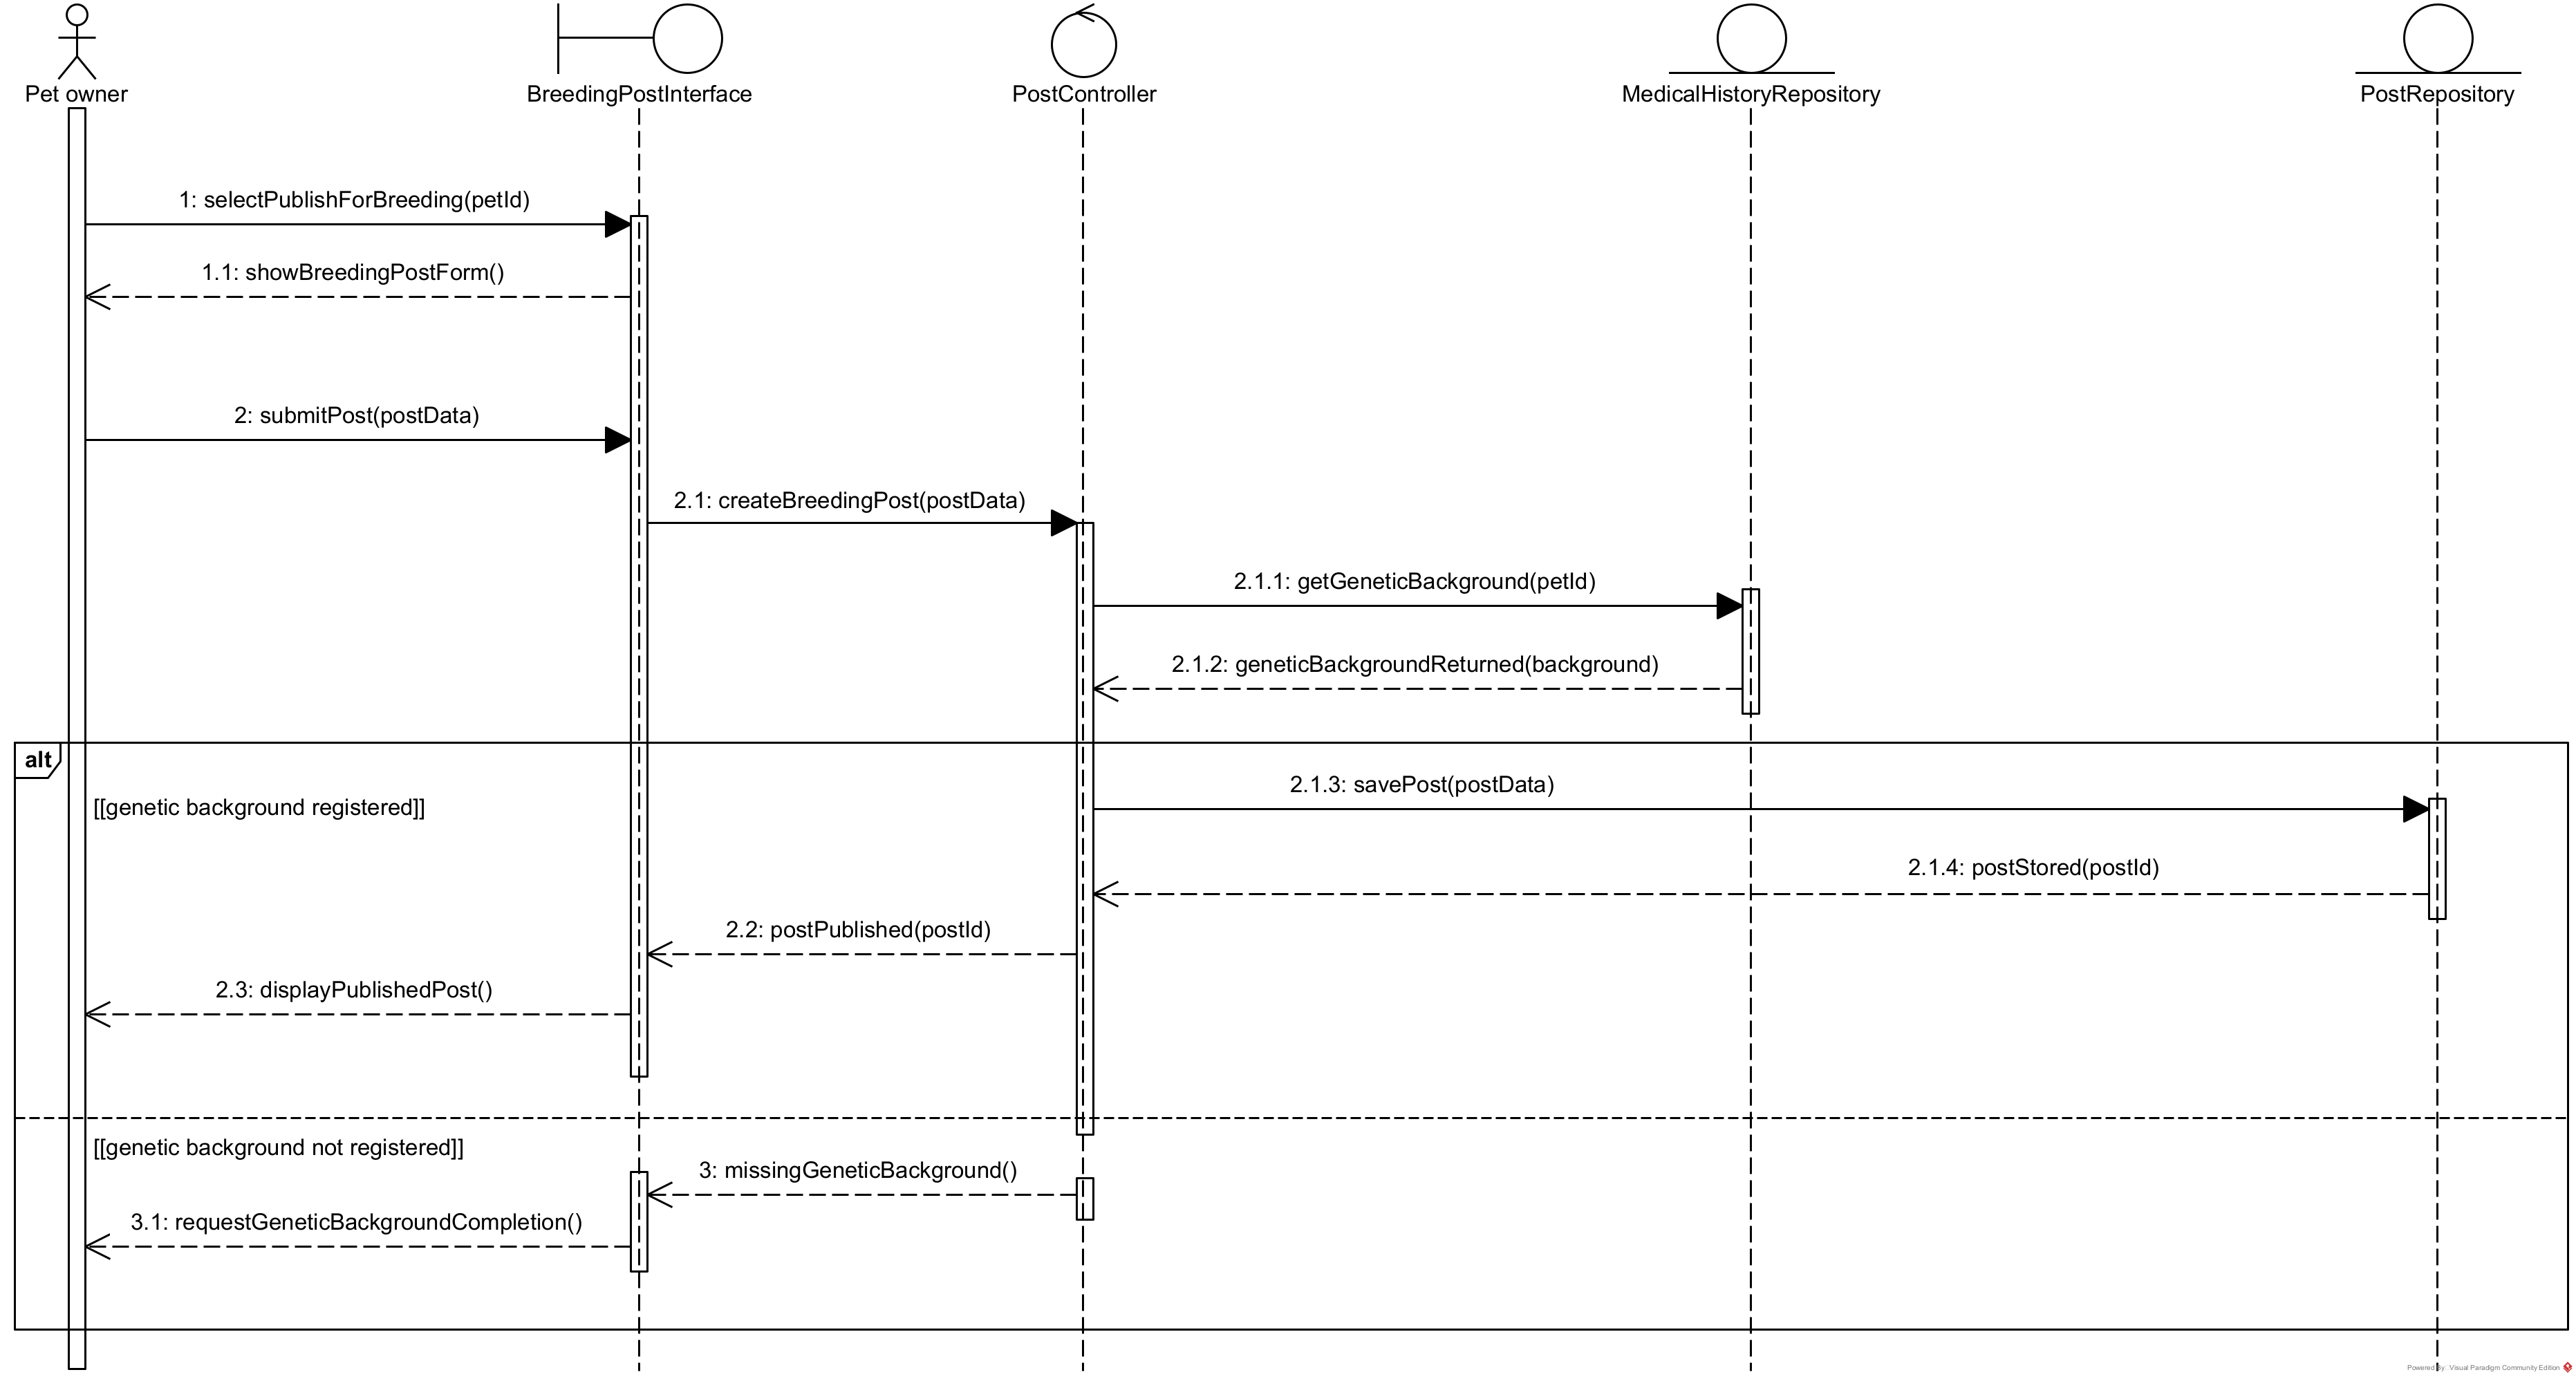
\includegraphics[width=0.95\textwidth]{DiagramaSecuencia_CU-05_MundiPets.png}
		\caption{Diagrama de secuencia -- Publicar mascota para cruza y gestionar solicitud (CU-05).}
		\label{fig:sec_cu05}
	\end{figure}
	
	Que \textit{getGeneticBackground(petId)} se consulte obligatoriamente
	antes de poder publicar (y bloquee la publicación en el camino ``genetic
	background not registered''), como se observa en la Figura~\ref{fig:sec_cu05},
	revela que la trazabilidad genética no es un campo opcional del
	formulario, sino una precondición dura para la cruza, materializando
	directamente el requisito de ``responsabilidad en la cruza'' declarado en
	el alcance de MundiPets. Esta dependencia obligatoria contrasta con el
	CU-04 (adopción), donde no existe tal barrera, mostrando que ambos
	procesos de publicación tienen niveles de exigencia distintos según el
	riesgo asociado.
	
	\subsubsection{Configurar privacidad médica (CU-06)}
	
	\begin{figure}[H]
		\centering
		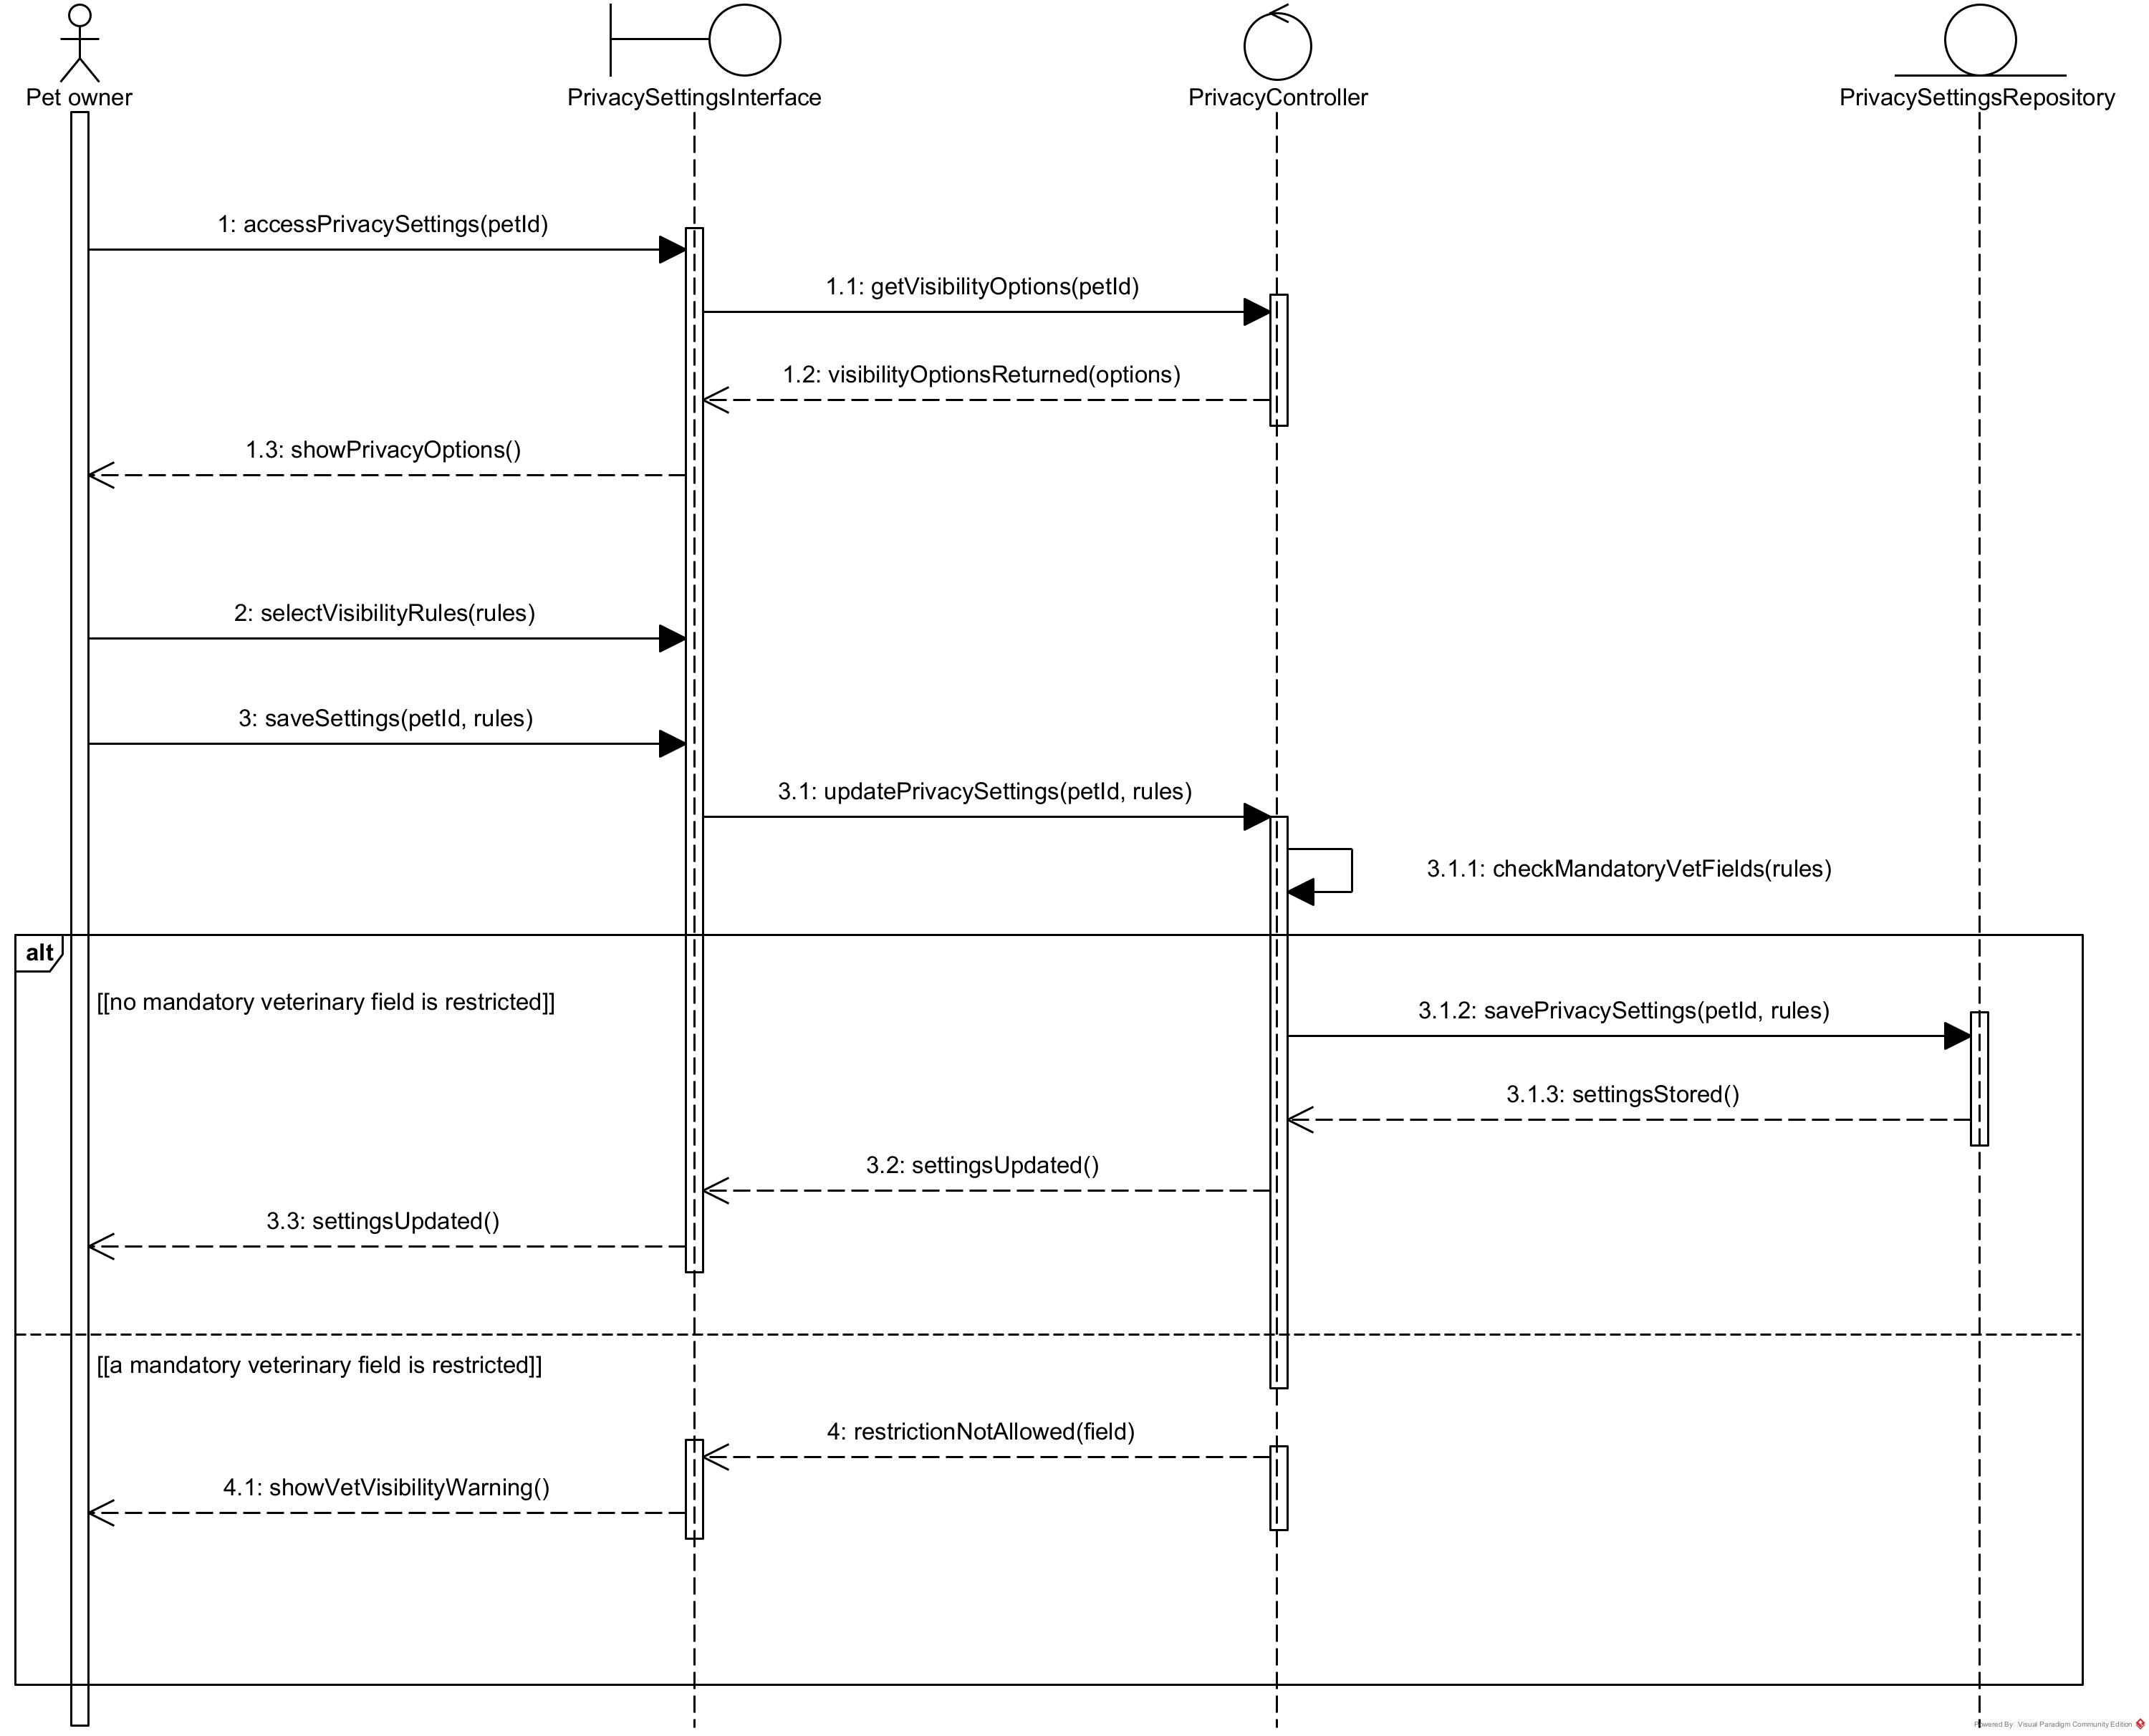
\includegraphics[width=0.95\textwidth]{DiagramaSecuencia_CU-06_MundiPets.png}
		\caption{Diagrama de secuencia -- Configurar privacidad médica (CU-06).}
		\label{fig:sec_cu06}
	\end{figure}
	
	Que \textit{checkMandatoryVetFields(rules)} sea una validación reflexiva
	del controlador que puede rechazar la solicitud del dueño (``a mandatory
	veterinary field is restricted''), tal como se ve en la
	Figura~\ref{fig:sec_cu06}, revela que la privacidad configurable por el
	usuario tiene un límite impuesto por el sistema: el dueño puede ocultar
	información no crítica, pero no puede restringir campos que la clínica
	veterinaria necesita ver para validar. Esto demuestra que la privacidad
	del dato médico no es absoluta, sino que está subordinada a la seguridad
	clínica del proceso.
	
	\subsubsection{Gestionar proceso de adopción (CU-07)}
	
	\begin{figure}[H]
		\centering
		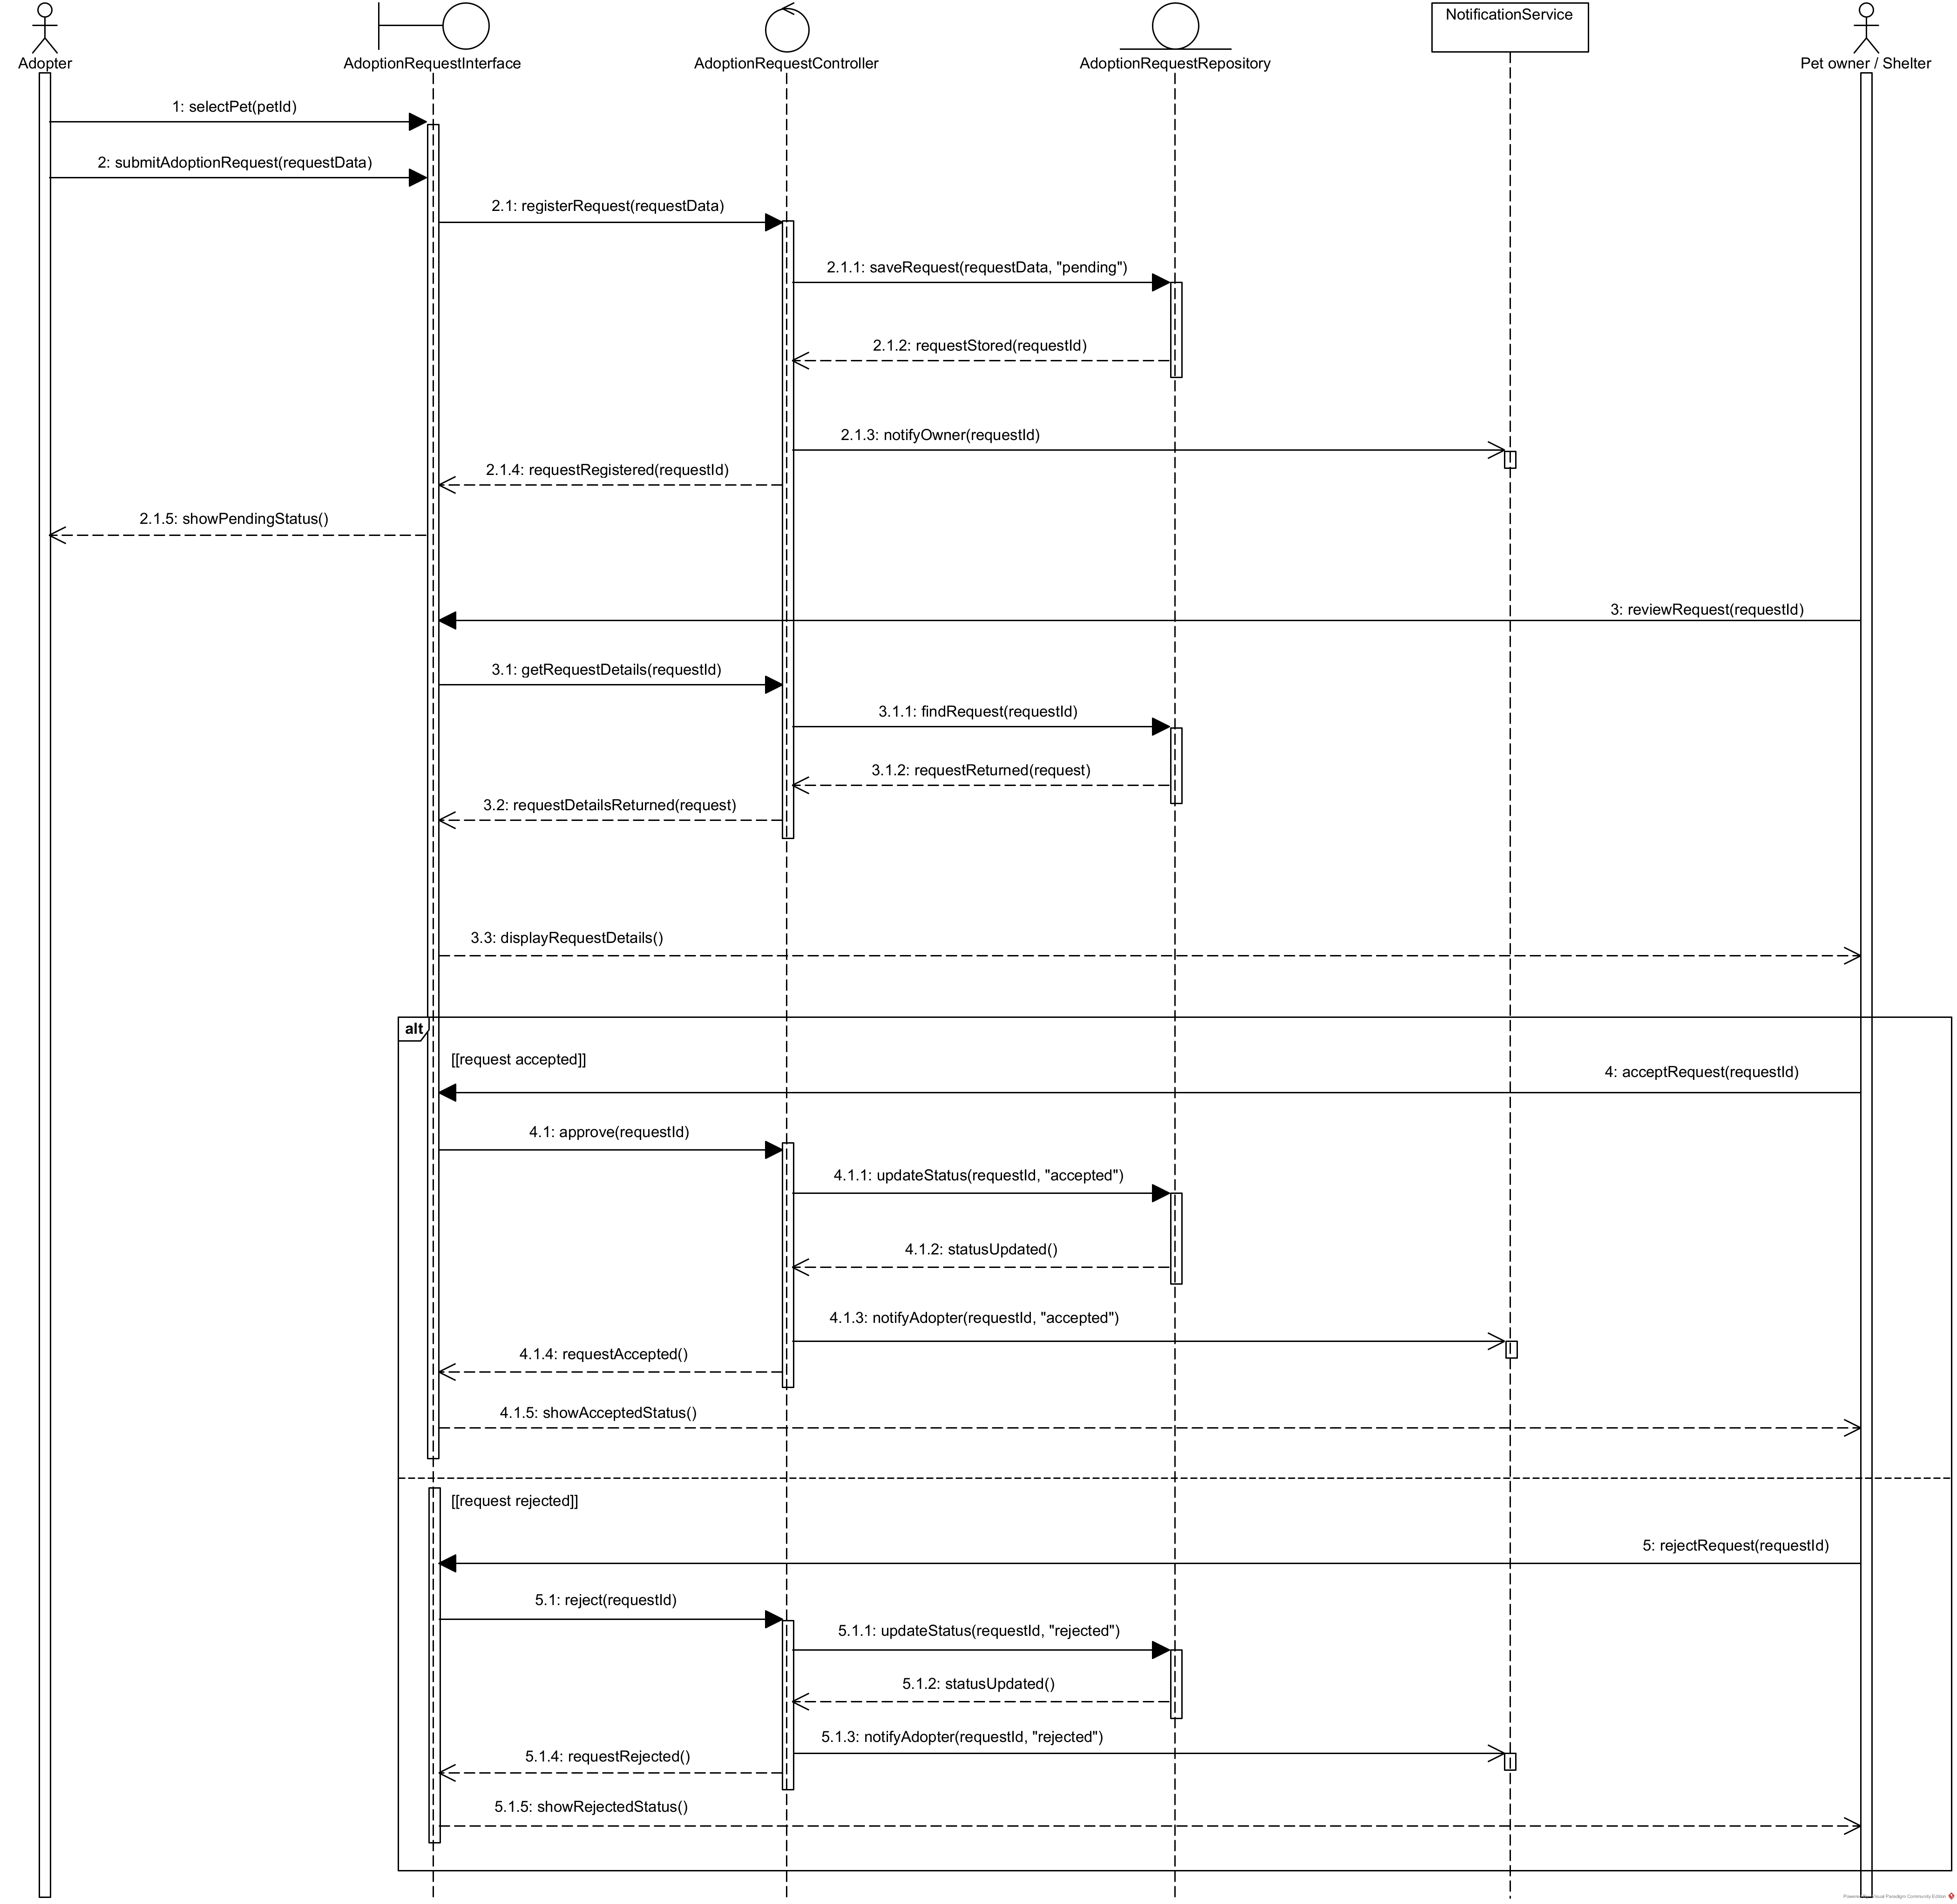
\includegraphics[width=0.95\textwidth]{DiagramaSecuencia_CU-07_MundiPets.png}
		\caption{Diagrama de secuencia -- Gestionar proceso de adopción (CU-07).}
		\label{fig:sec_cu07}
	\end{figure}
	
	Que \textit{notifyOwner}/\textit{notifyAdopter} se disparen en cada
	transición de estado (registro, aceptación, rechazo) a través de un
	\textit{NotificationService} externo y compartido, en lugar de que cada
	actor consulte manualmente el estado, según se ve en la
	Figura~\ref{fig:sec_cu07}, revela que el proceso de adopción se diseñó
	como orientado a eventos: ningún cambio de estado ocurre en silencio. Que
	el \textit{alt} solo contemple ``accepted'' o ``rejected'' como
	desenlaces (sin una rama de ``cancelado'' en este mismo diagrama) muestra
	que la cancelación se modela por separado (coherente con la máquina de
	estados de Solicitudes, Figura~\ref{fig:me_solicitudes}), evitando que
	este diagrama de secuencia intente cubrir cada excepción del ciclo de
	vida completo.
	
	\subsubsection{Gestionar comunicación entre usuarios (CU-08)}
	
	\begin{figure}[H]
		\centering
		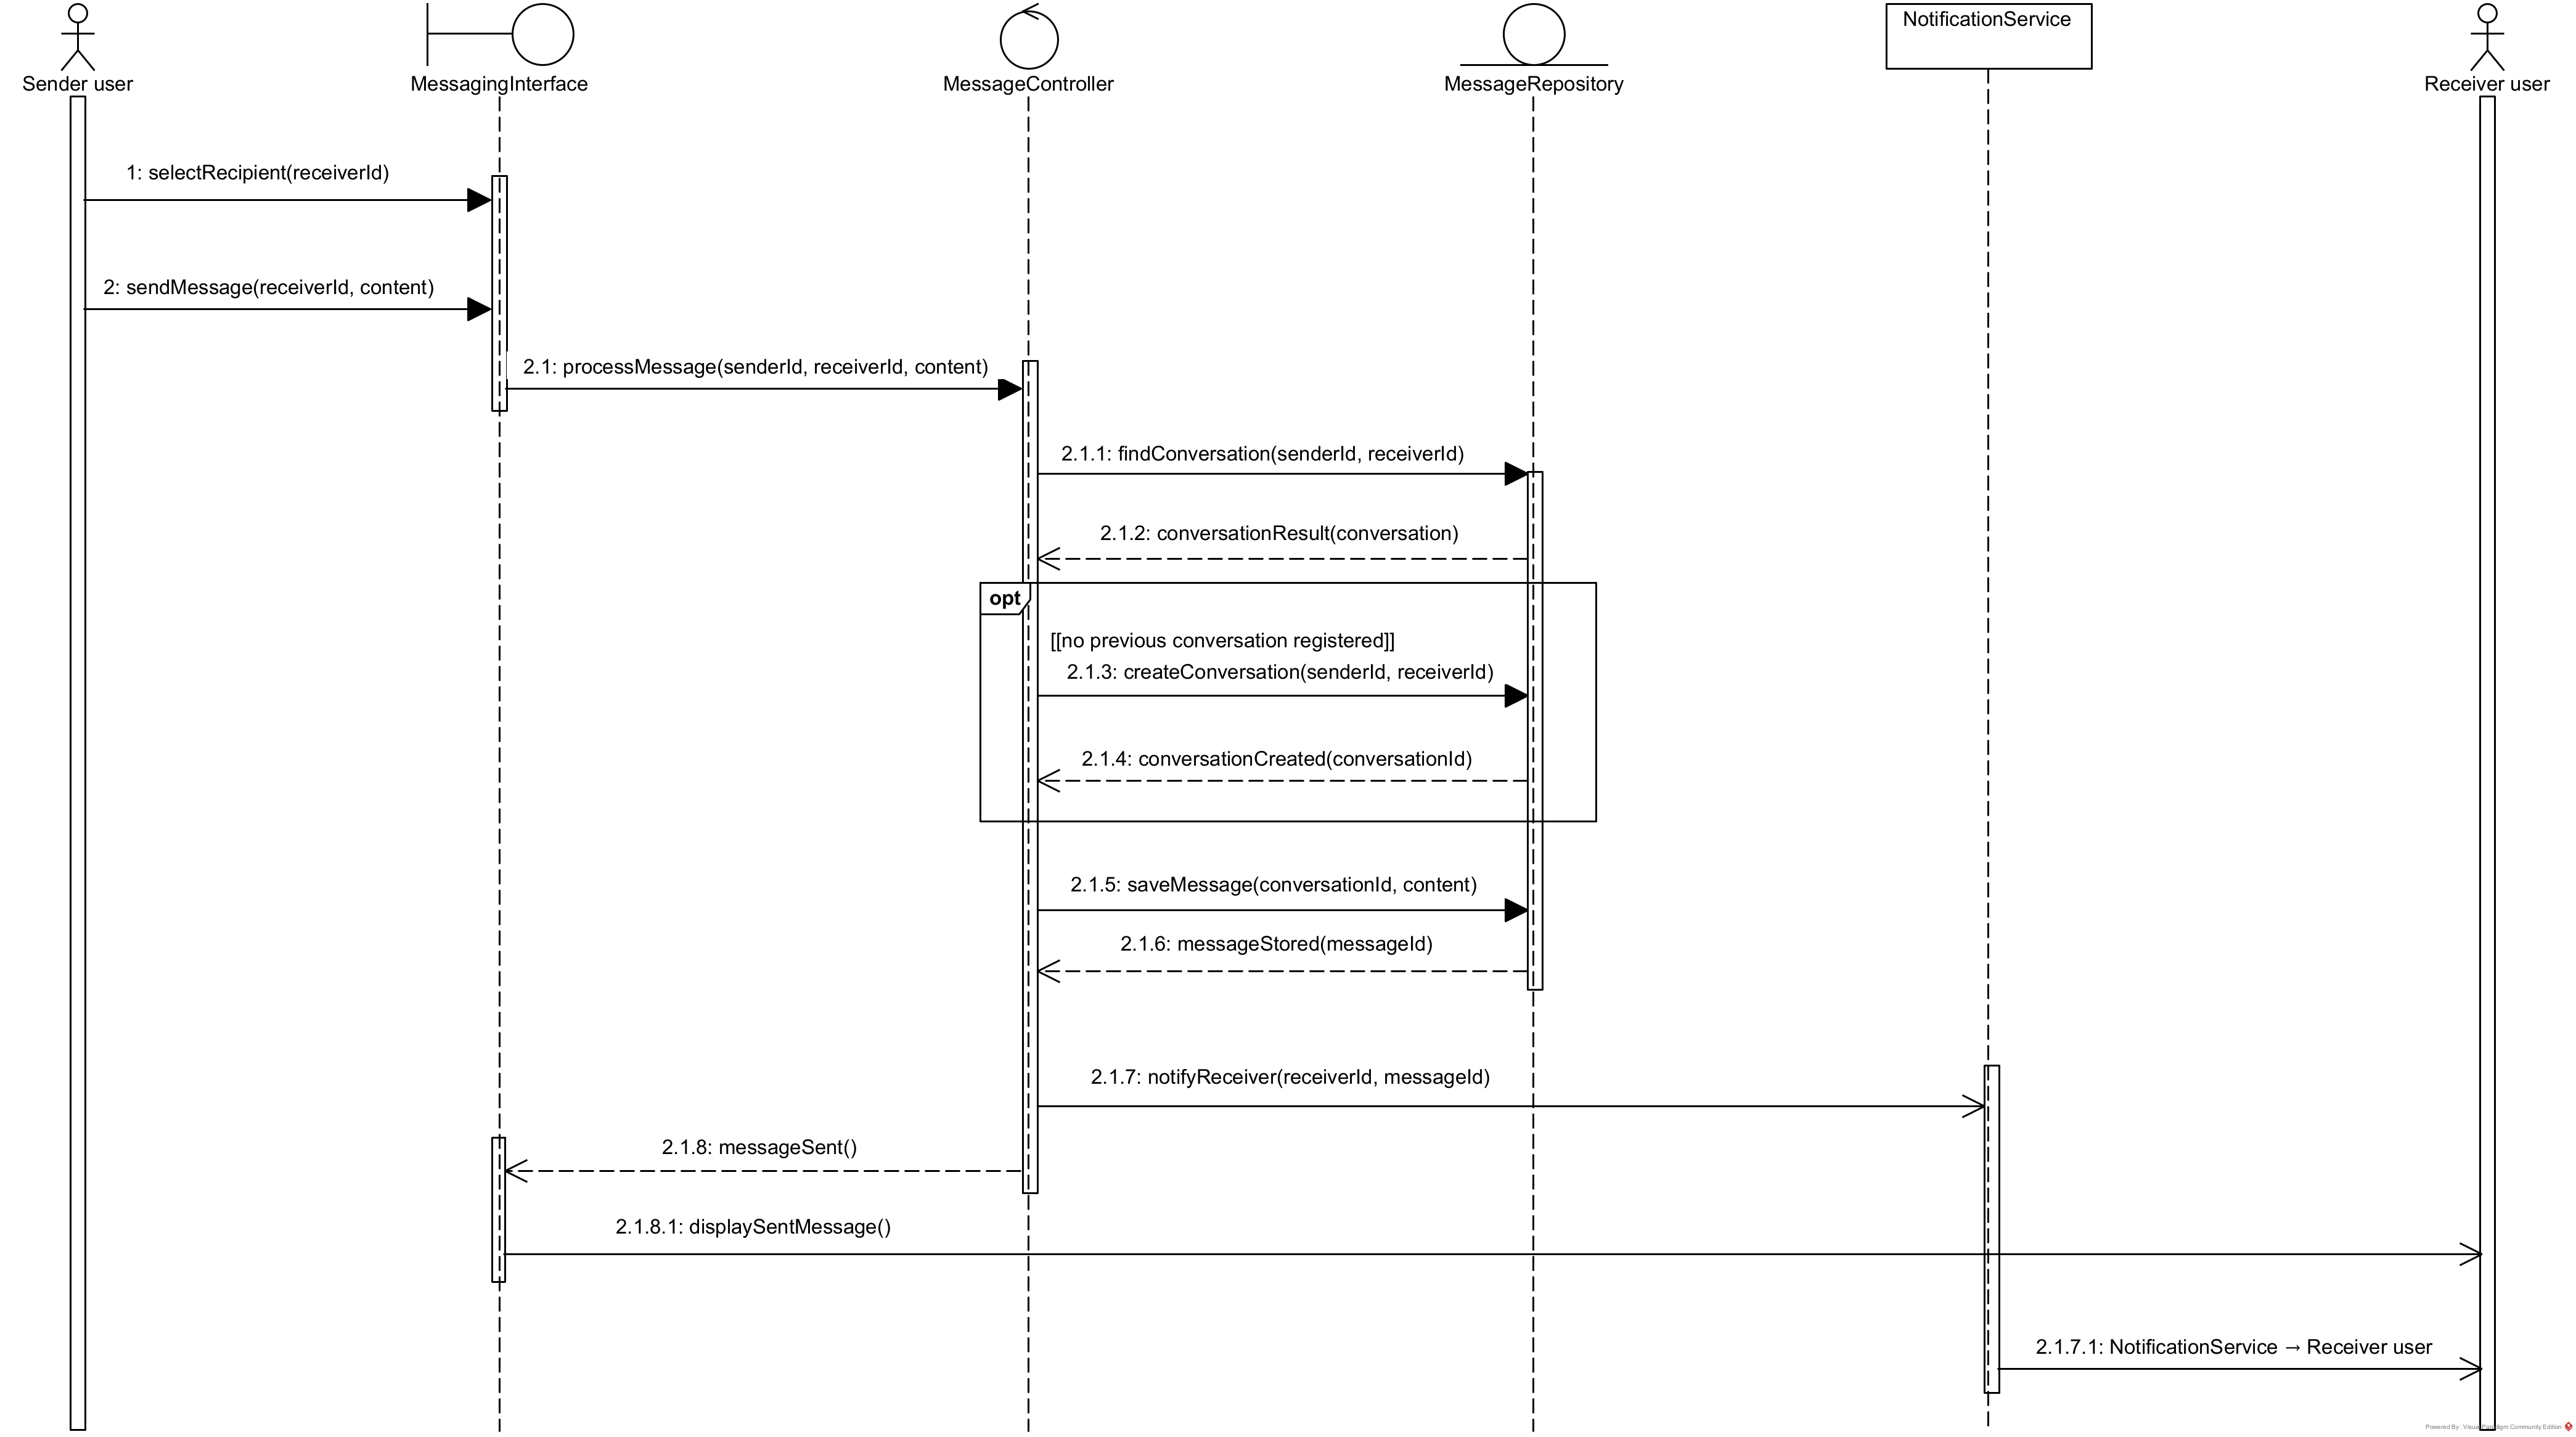
\includegraphics[width=0.95\textwidth]{DiagramaSecuencia_CU-08_MundiPets.png}
		\caption{Diagrama de secuencia -- Gestionar comunicación entre usuarios (CU-08).}
		\label{fig:sec_cu08}
	\end{figure}
	
	Que \textit{createConversation} esté envuelto en un bloque \textit{opt}
	condicionado a ``no previous conversation registered'' (y no se ejecute
	siempre), como se observa en la Figura~\ref{fig:sec_cu08}, revela que el
	sistema modela la conversación como una entidad persistente y reutilizable
	entre dos usuarios, evitando fragmentar el historial de mensajes en hilos
	nuevos cada vez que alguien escribe. Que \textit{notifyReceiver} ocurra
	después de \textit{messageStored} (nunca antes) muestra que el sistema
	garantiza la persistencia del mensaje como condición previa a cualquier
	notificación, evitando alertar de algo que aún podría fallar al
	guardarse.
	
	\subsubsection{Validar información médica (CU-09)}
	
	\begin{figure}[H]
		\centering
		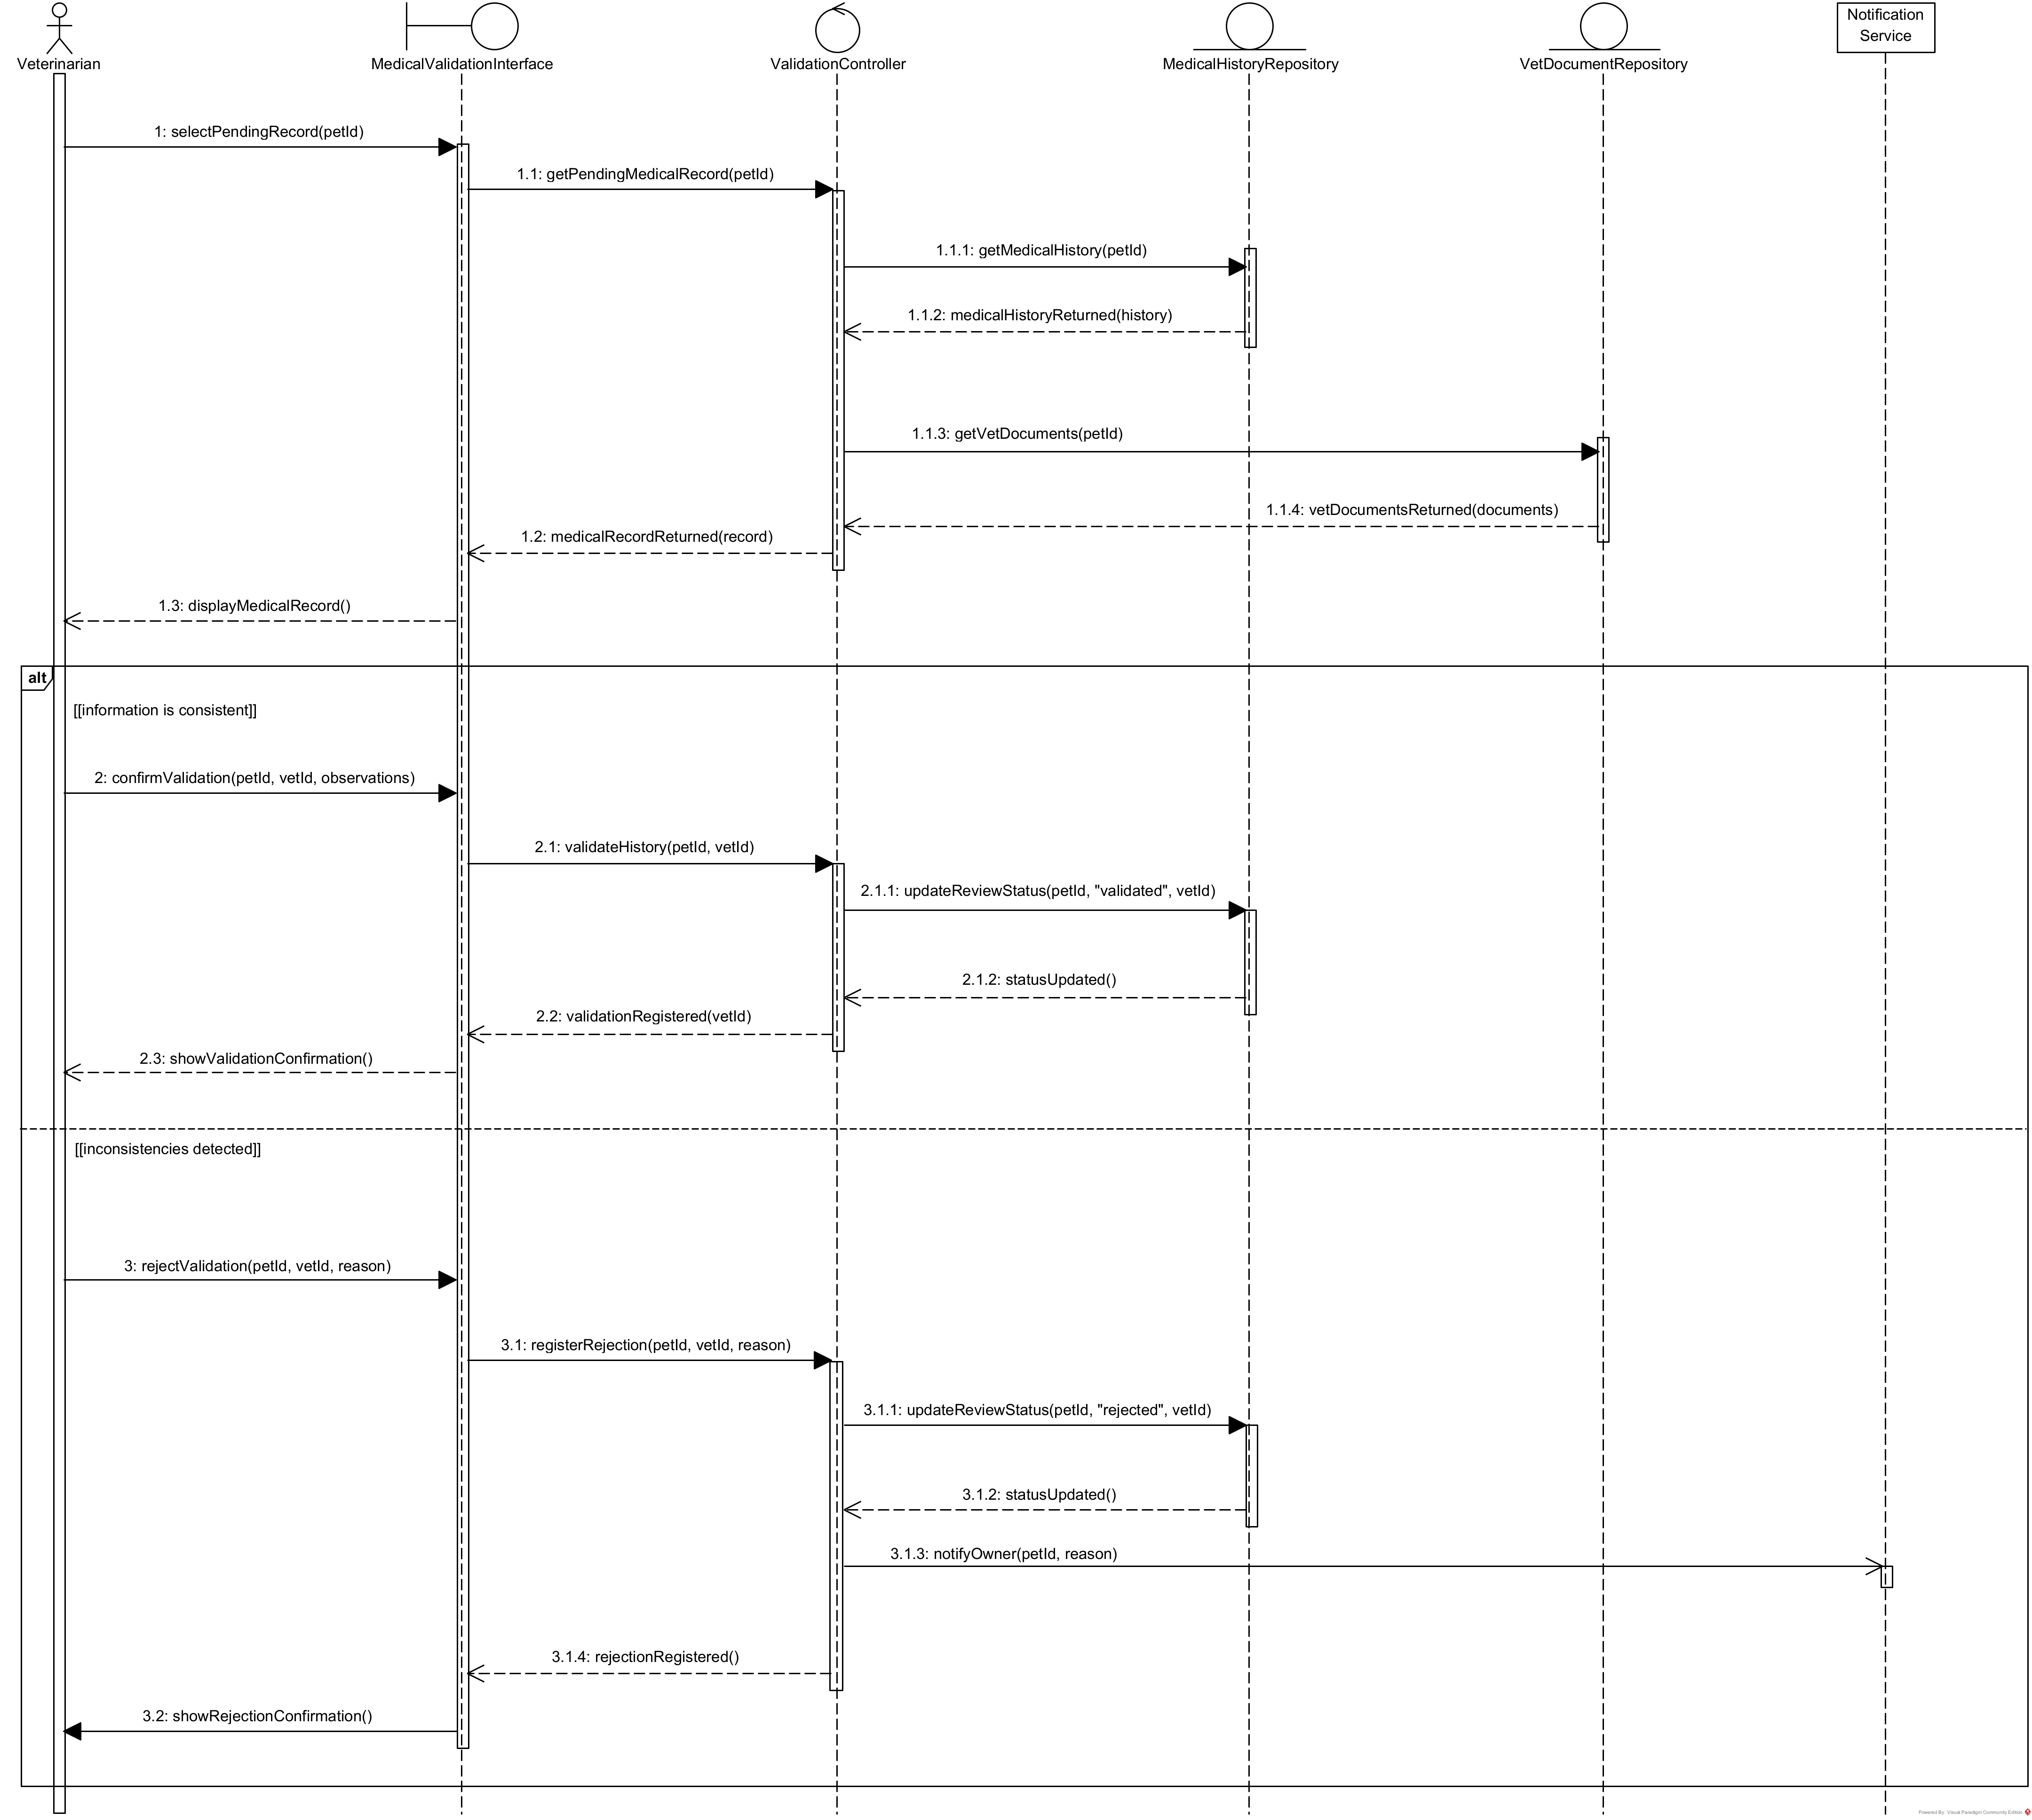
\includegraphics[width=0.95\textwidth]{DiagramaSecuencia_CU-09_MundiPets.png}
		\caption{Diagrama de secuencia -- Validar información médica (CU-09).}
		\label{fig:sec_cu09}
	\end{figure}
	
	Que el veterinario reciba tanto \textit{getMedicalHistory} como
	\textit{getVetDocuments} en paralelo desde dos repositorios distintos
	antes de emitir cualquier veredicto, tal como se ve en la
	Figura~\ref{fig:sec_cu09}, revela que la validación clínica exige cruzar
	la información declarada por el dueño con el documento formal adjunto, y
	no aceptar ninguna de las dos fuentes de forma aislada. Que el
	\textit{alt} solo ofrezca ``validated'' o ``rejected'' (sin estado
	intermedio) y que el rechazo dispare \textit{notifyOwner(petId, reason)}
	con motivo explícito, refleja que el sistema exige trazabilidad del
	porqué de un rechazo, no solo el hecho de que ocurrió, coherente con la
	máquina de estados de Verificación de Documentos (Figura~\ref{fig:me_verificacion}).
	
	\subsubsection{Consultar perfil médico (CU-10)}
	
	\begin{figure}[H]
		\centering
		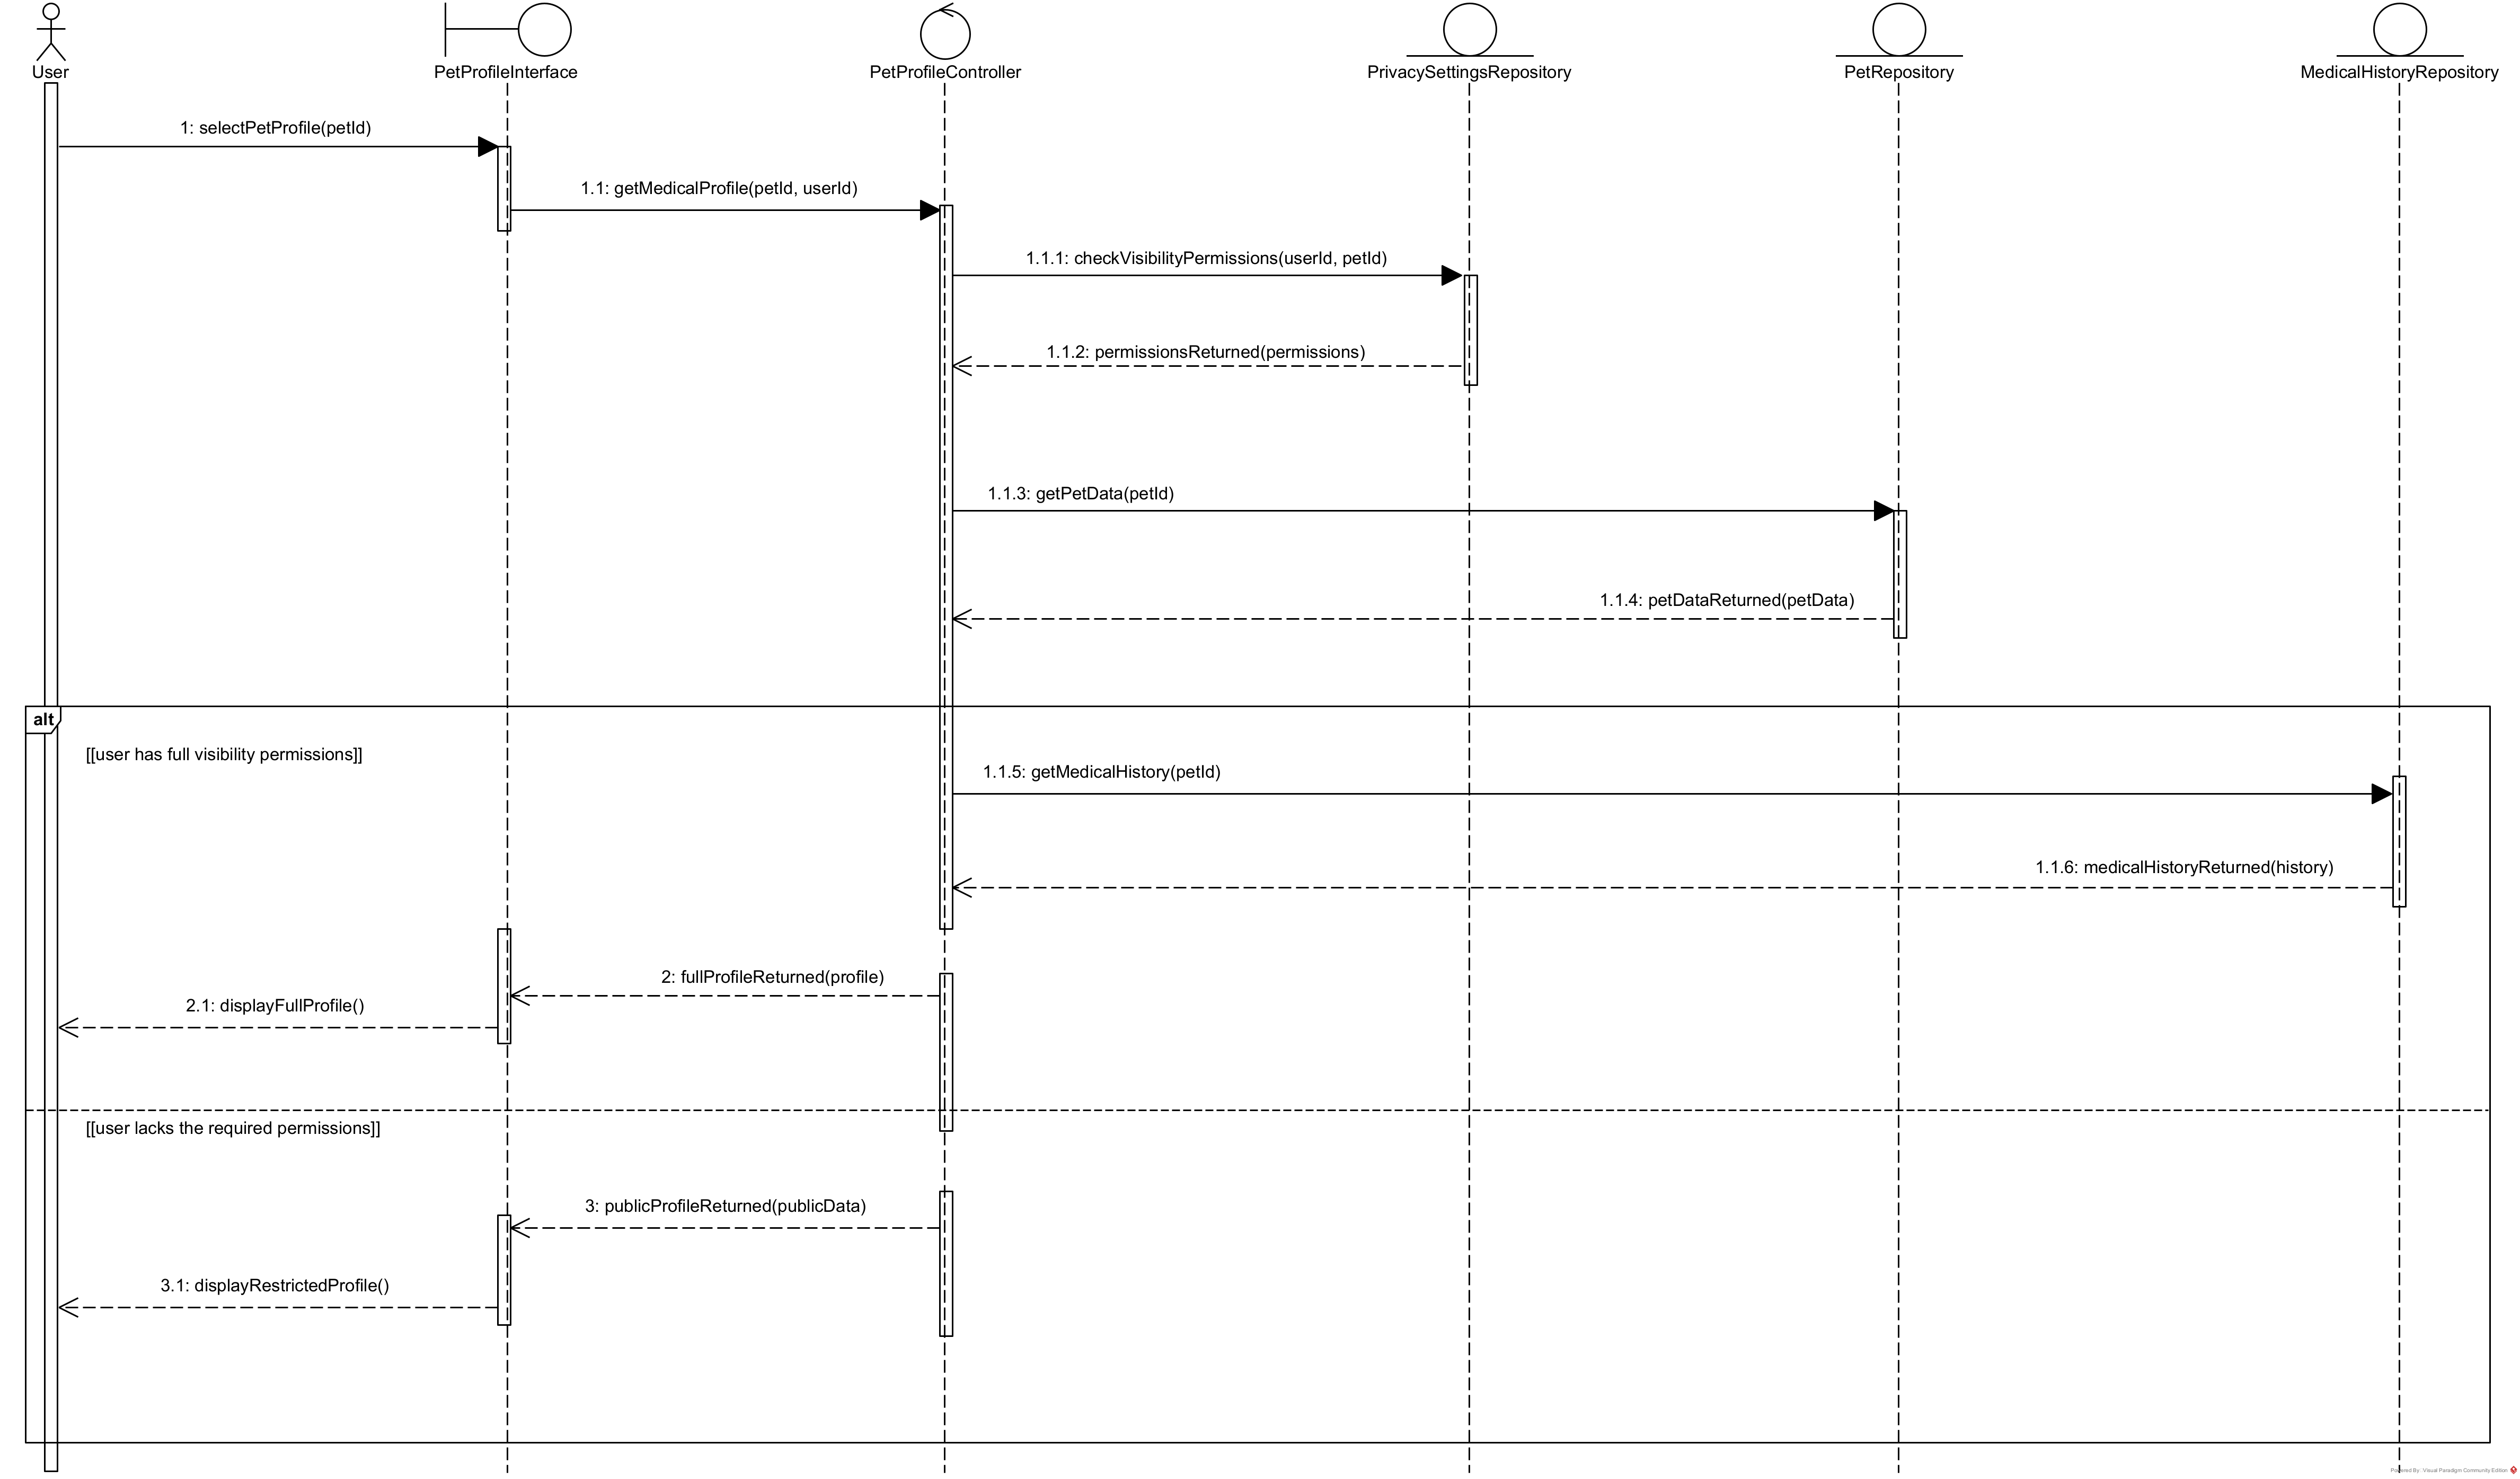
\includegraphics[width=0.95\textwidth]{DiagramaSecuencia_CU-10_MundiPets.png}
		\caption{Diagrama de secuencia -- Consultar perfil médico (CU-10).}
		\label{fig:sec_cu10}
	\end{figure}
	
	Que \textit{checkVisibilityPermissions(userId, petId)} se ejecute antes
	de decidir si se llama a \textit{getMedicalHistory} (el \textit{alt}
	separa ``full visibility permissions'' de ``lacks the required
	permissions''), como se observa en la Figura~\ref{fig:sec_cu10}, revela
	que el perfil médico no es un dato binario visible/oculto, sino que el
	propio controlador construye una respuesta distinta según el
	solicitante: la información sensible ni siquiera se consulta si el
	usuario no tiene permiso, en vez de consultarla y luego filtrarla. Esto
	materializa directamente el CU-06 (Figura~\ref{fig:sec_cu06}): ambos
	diagramas comparten la misma fuente de reglas
	(\textit{PrivacySettingsRepository}).
	
	\subsubsection{Buscar mascota disponible (CU-11)}
	
	\begin{figure}[H]
		\centering
		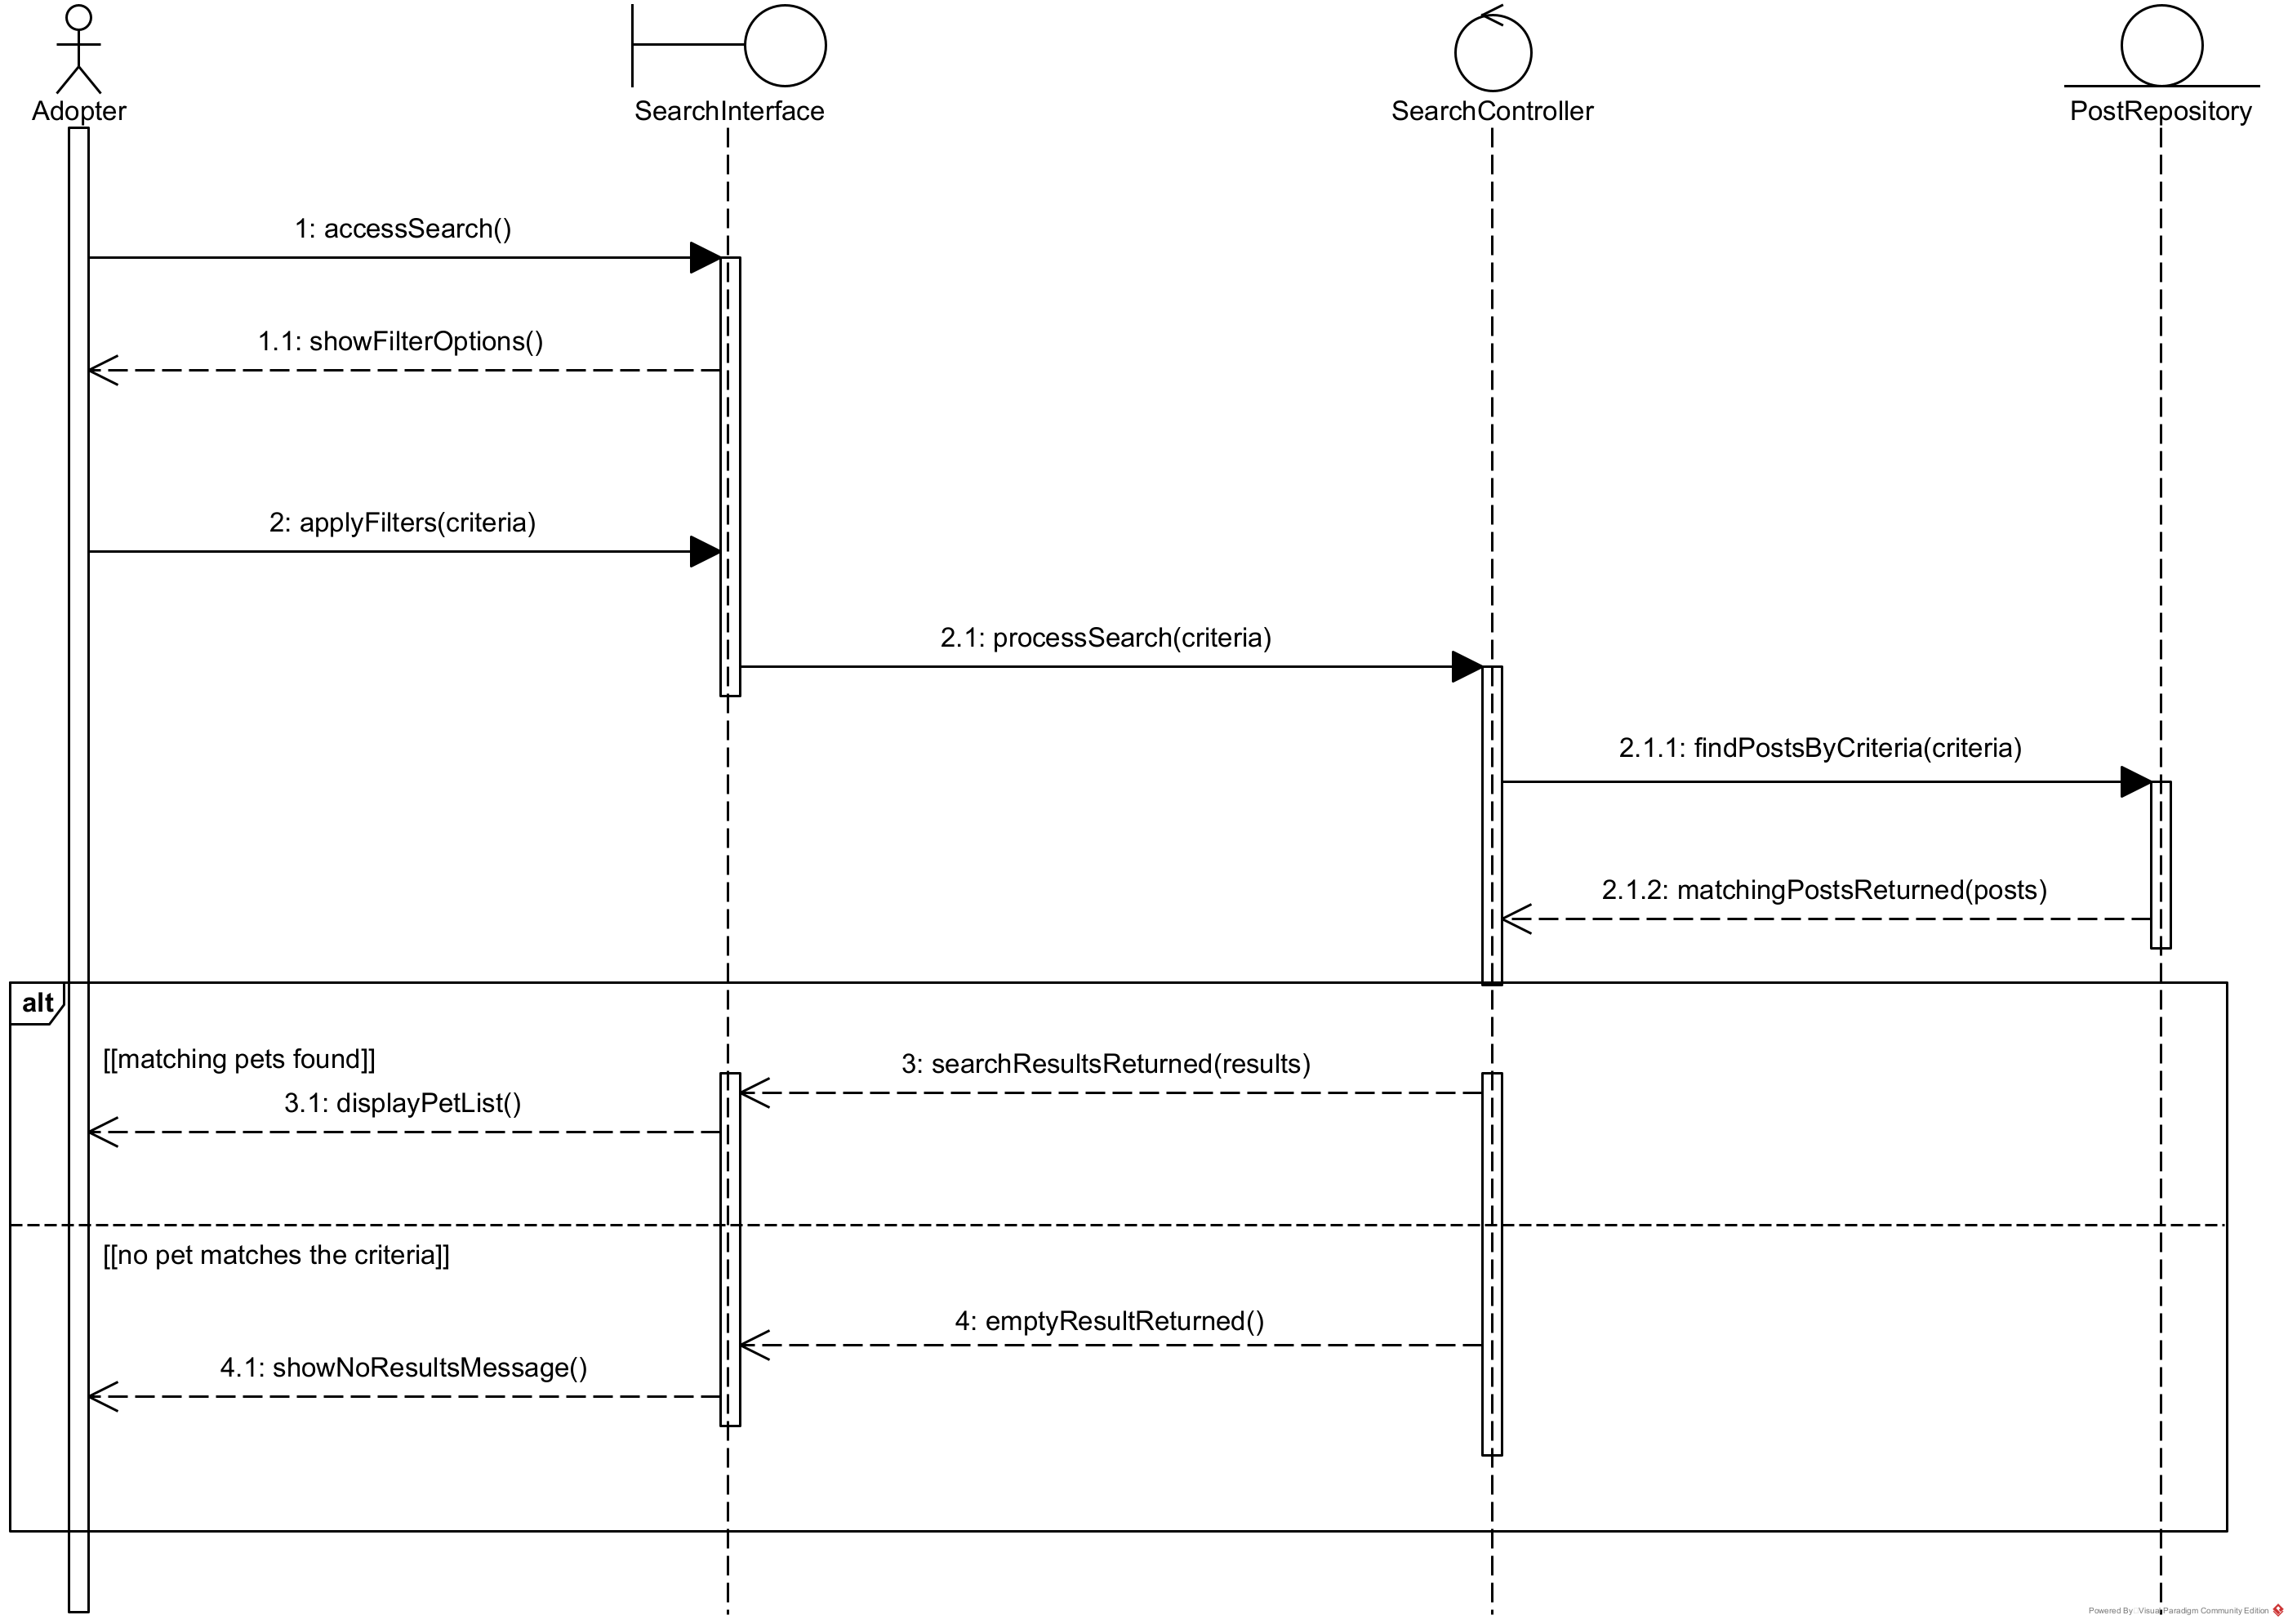
\includegraphics[width=0.95\textwidth]{DiagramaSecuencia_CU-11_MundiPets.png}
		\caption{Diagrama de secuencia -- Buscar mascota disponible (CU-11).}
		\label{fig:sec_cu11}
	\end{figure}
	
	Que el \textit{alt} distinga entre ``matching pets found'' y ``no pet
	matches the criteria'' como dos resultados igualmente válidos de una
	búsqueda (y no un error), tal como se ve en la Figura~\ref{fig:sec_cu11},
	revela que el sistema trata la ausencia de resultados como un estado de
	negocio esperado y comunicable (\textit{showNoResultsMessage}), no como
	una excepción a capturar. La simplicidad del flujo (sin bloque de
	validación de errores de entrada) muestra que este caso de uso confía en
	que los filtros de búsqueda siempre producen criterios sintácticamente
	válidos, delegando esa validación a la capa de interfaz.
	
	\subsubsection{Consultar recomendaciones de cuidado (CU-12)}
	
	\begin{figure}[H]
		\centering
		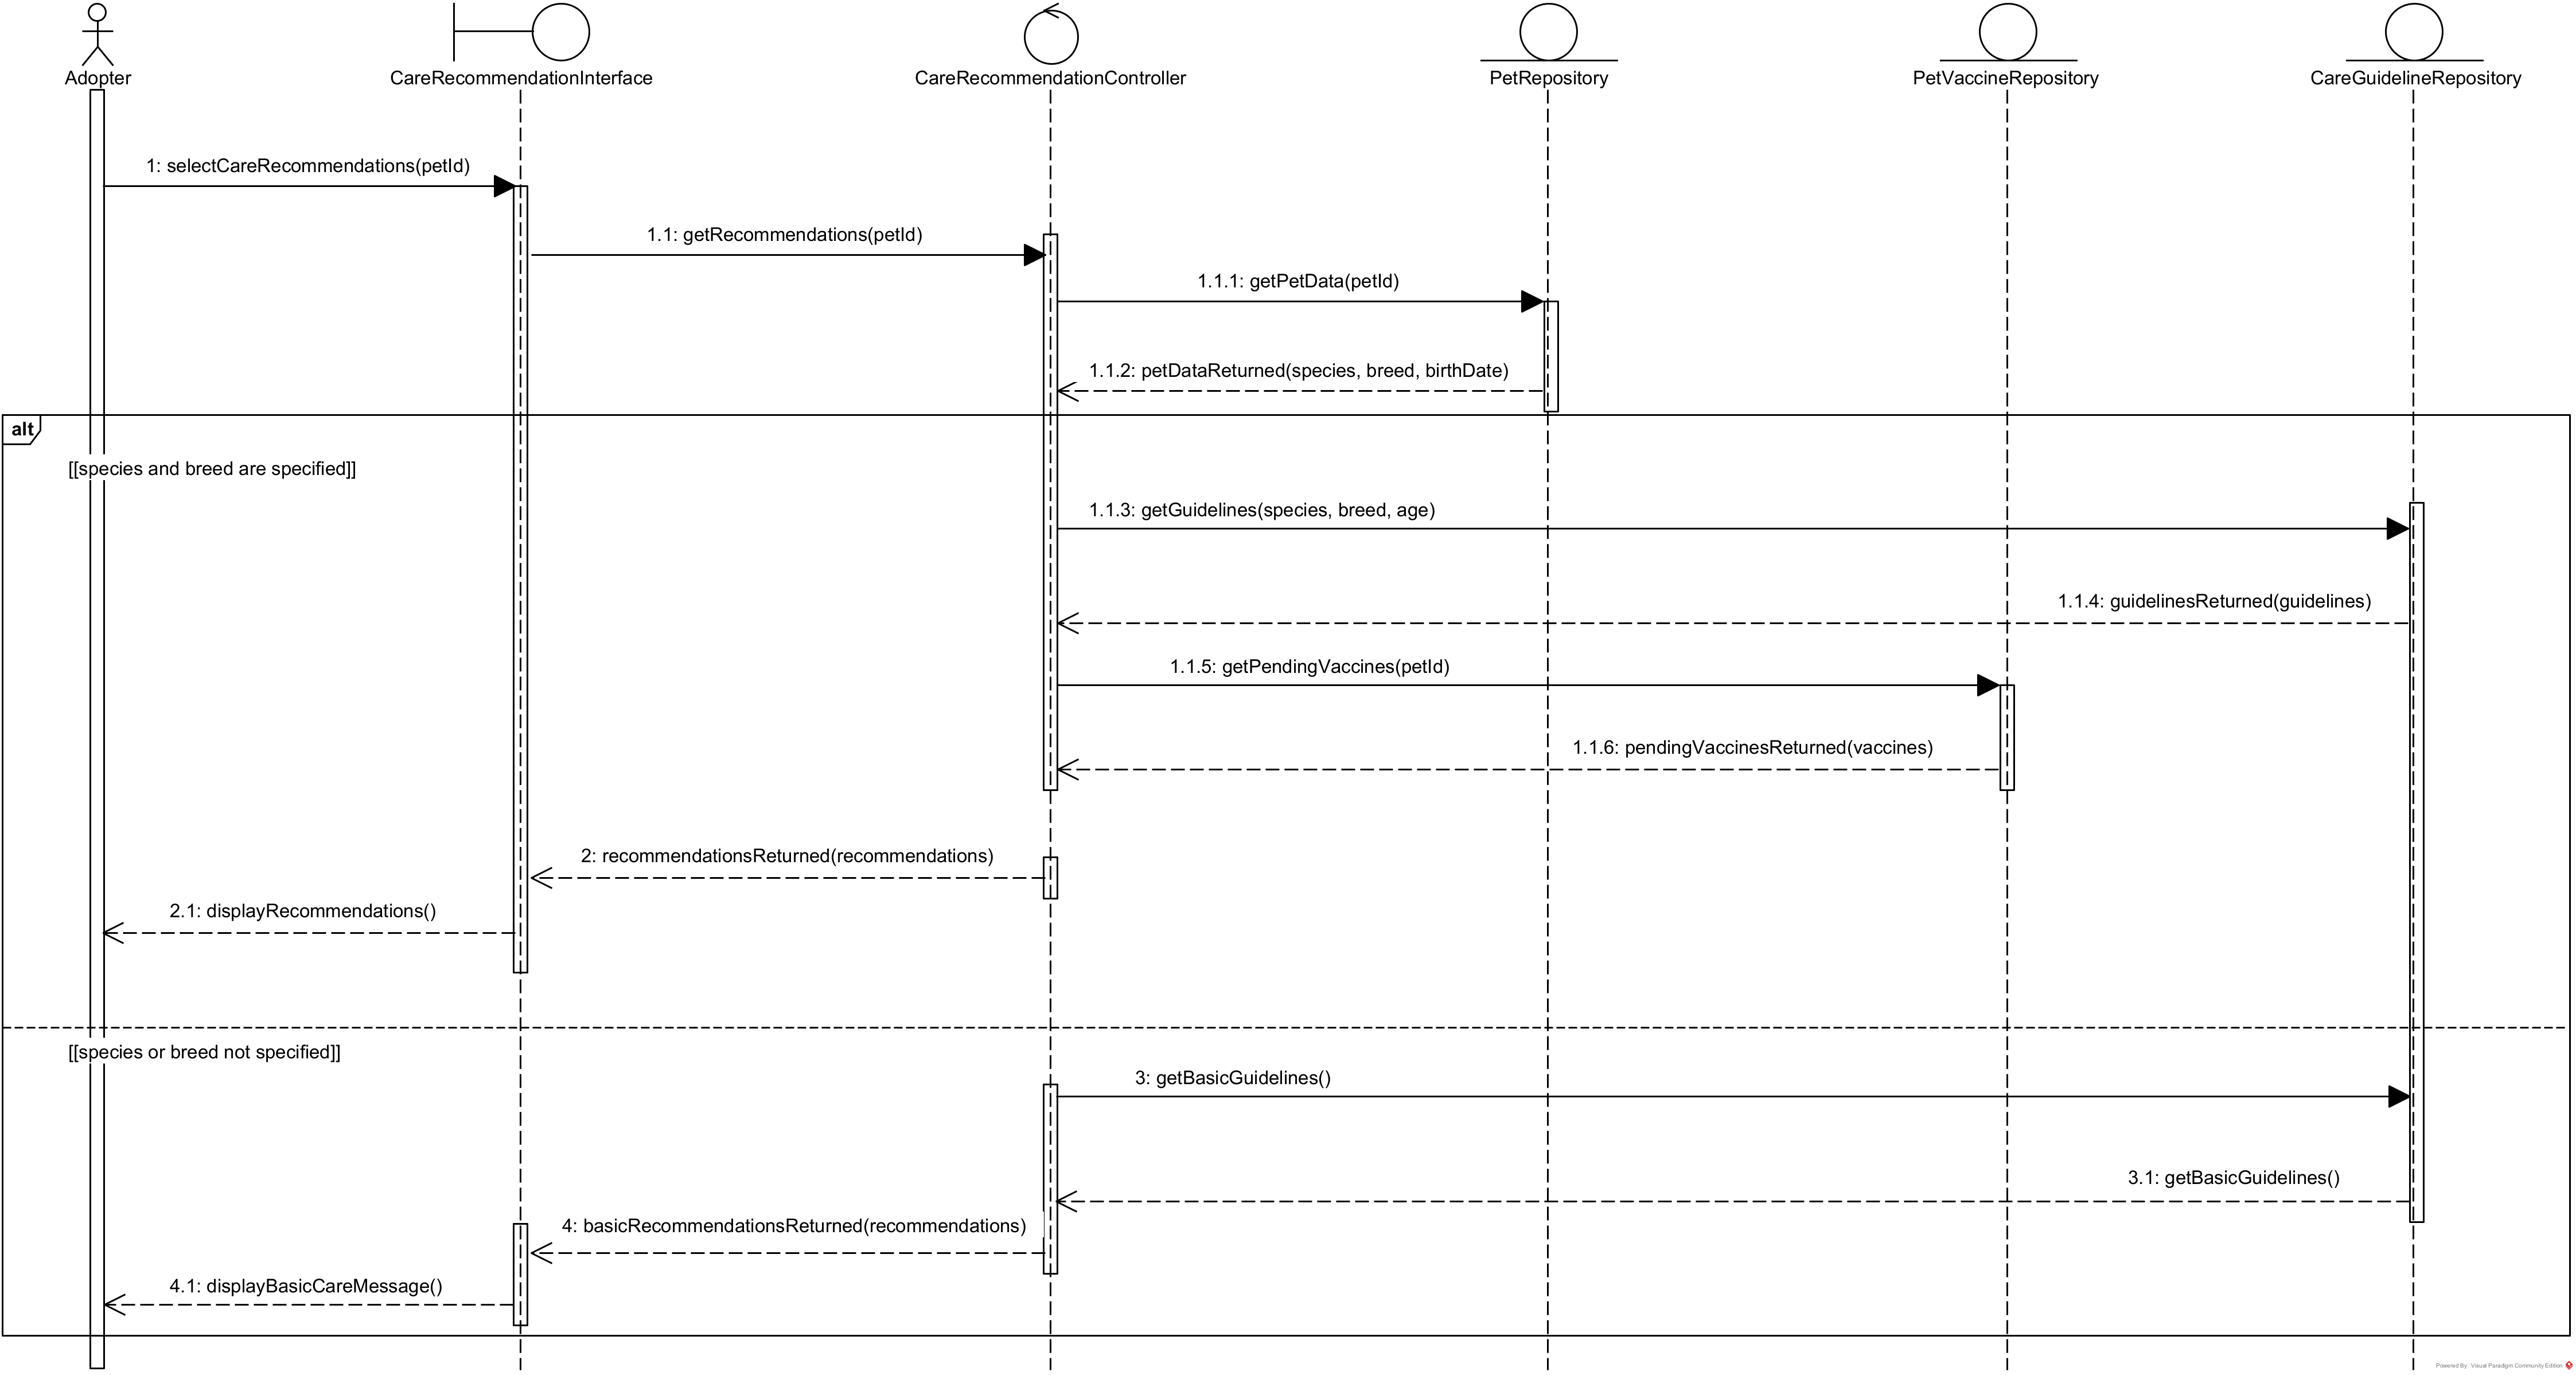
\includegraphics[width=0.95\textwidth]{DiagramaSecuencia_CU-12_MundiPets.png}
		\caption{Diagrama de secuencia -- Consultar recomendaciones de cuidado (CU-12).}
		\label{fig:sec_cu12}
	\end{figure}
	
	Que el \textit{alt} dependa de si ``species and breed are specified'' y
	no de si el usuario las proporcionó explícitamente en este momento (los
	datos ya vienen de \textit{getPetData}), como se observa en la
	Figura~\ref{fig:sec_cu12}, revela que las recomendaciones de cuidado
	dependen de la calidad de los datos previamente registrados del perfil,
	no de una nueva entrada del adoptante: si el perfil está incompleto, el
	sistema degrada a \textit{getBasicGuidelines()} en lugar de bloquear la
	función. Esta decisión de tener un camino de \textit{fallback} con
	recomendaciones genéricas, en vez de negar el servicio, refleja que la
	utilidad de la funcionalidad se prioriza sobre la exhaustividad de los
	datos.
	
	\subsubsection{Evaluar compatibilidad de cruza (CU-13)}
	
	\begin{figure}[H]
		\centering
		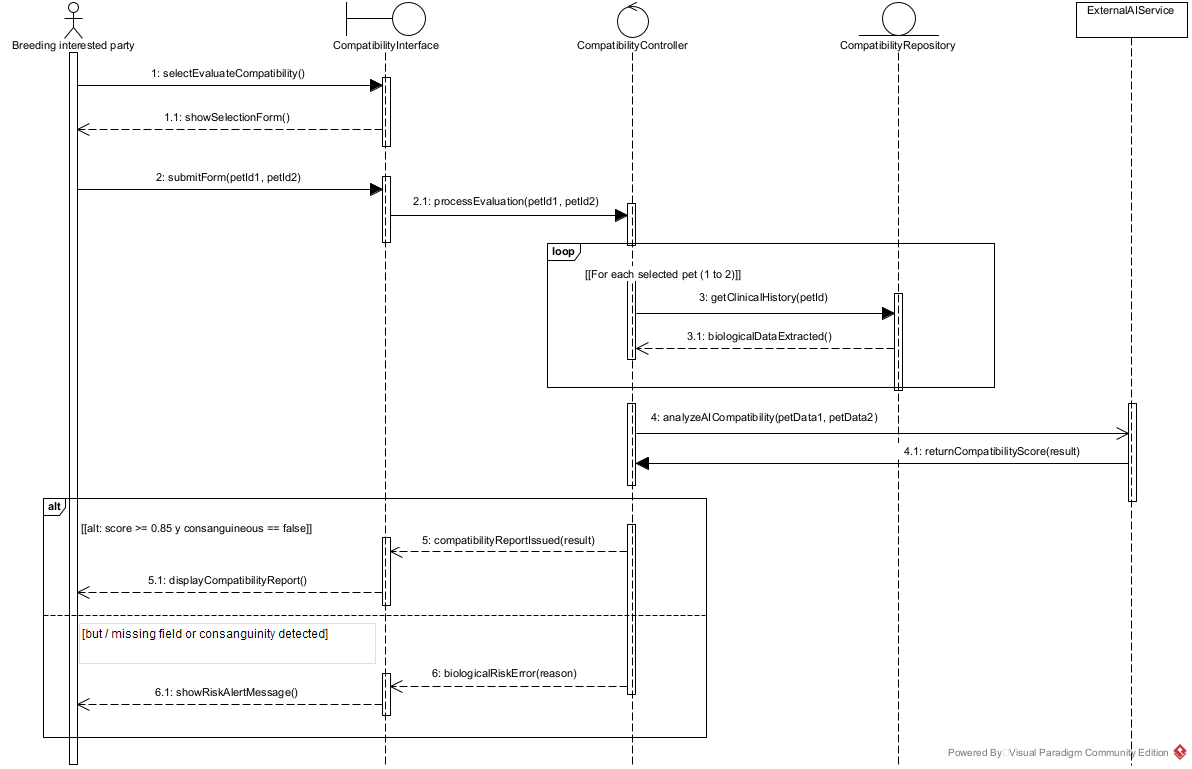
\includegraphics[width=0.95\textwidth]{DiagramaSecuencia_CU-13_MundiPets.png}
		\caption{Diagrama de secuencia -- Evaluar compatibilidad de cruza (CU-13).}
		\label{fig:sec_cu13}
	\end{figure}
	
	Que el \textit{loop} recorra los historiales clínicos de ambas mascotas
	(1 a 2) antes de invocar al \textit{ExternalAIService}, y que la
	condición del \textit{alt} combine dos criterios distintos
	(\textit{score >= 0.85} y \textit{consanguineous == false}) en vez de
	basarse solo en el puntaje de la IA, tal como se ve en la
	Figura~\ref{fig:sec_cu13}, revela que la recomendación de un componente
	probabilístico nunca es la única barrera de decisión: existe una regla
	determinista de consanguinidad que puede anular un buen puntaje de
	compatibilidad. Esto es la aplicación directa del límite declarado en la
	Sección~\ref{sec:req_ia} (``no reemplaza la evaluación veterinaria
	profesional''): la IA aporta una señal, pero una regla de negocio dura
	puede vetarla.
	
	% ------------------------------------------------------------
	\subsection{Diagramas de Actividad}
	
	\subsubsection{Registrar mascota (CU-01)}
	
	\begin{figure}[H]
		\centering
		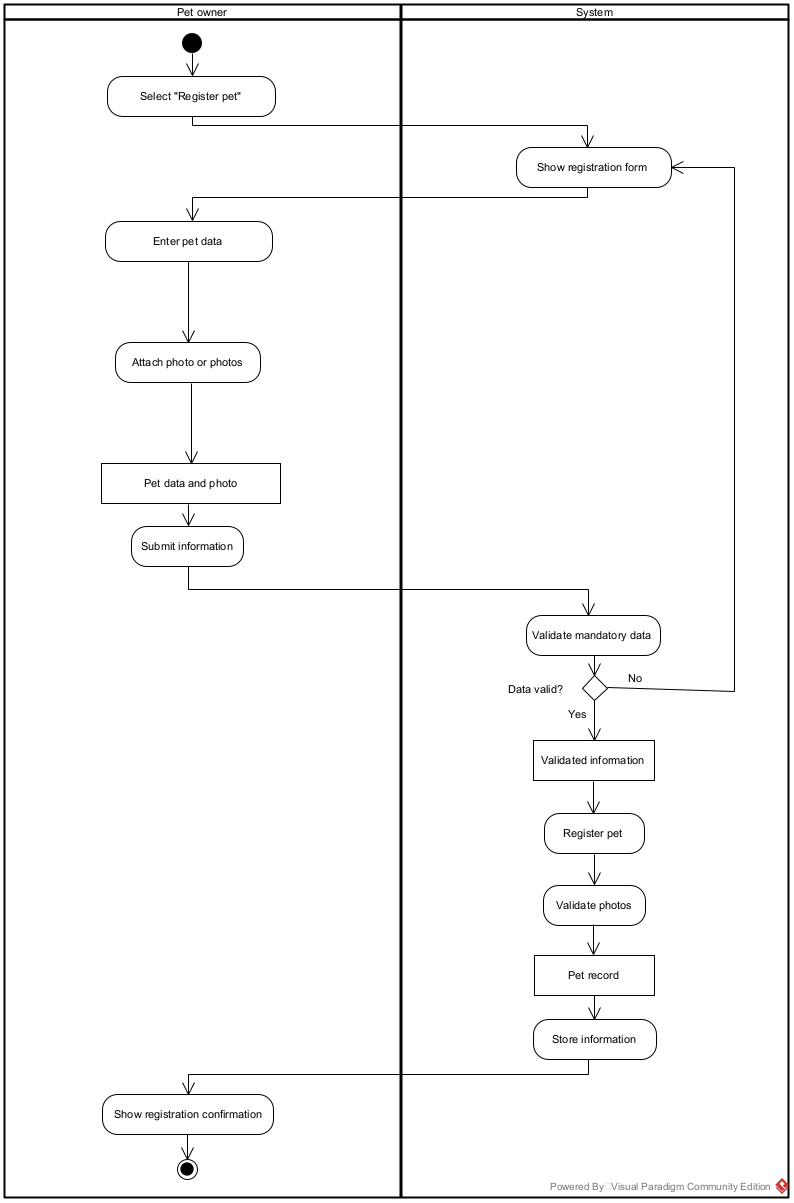
\includegraphics[width=0.55\textwidth]{DiagramaActividades_CU-01_MundiPets.png}
		\caption{Diagrama de actividades -- Registrar mascota (CU-01).}
		\label{fig:act_cu01}
	\end{figure}
	
	Que la validación ``Data valid?'' con salida ``No'' regrese al inicio
	del carril \textit{System} (``Show registration form'') y no simplemente
	muestre un mensaje de error puntual, como se ve en la Figura~\ref{fig:act_cu01},
	revela que el sistema fuerza al dueño a repetir el ciclo completo de
	llenado en lugar de corregir solo el campo fallido, priorizando la
	simplicidad de implementación sobre la fricción del usuario en esta
	primera versión del flujo.
	
	\subsubsection{Registrar historial médico y antecedentes genéticos (CU-02)}
	
	\begin{figure}[H]
		\centering
		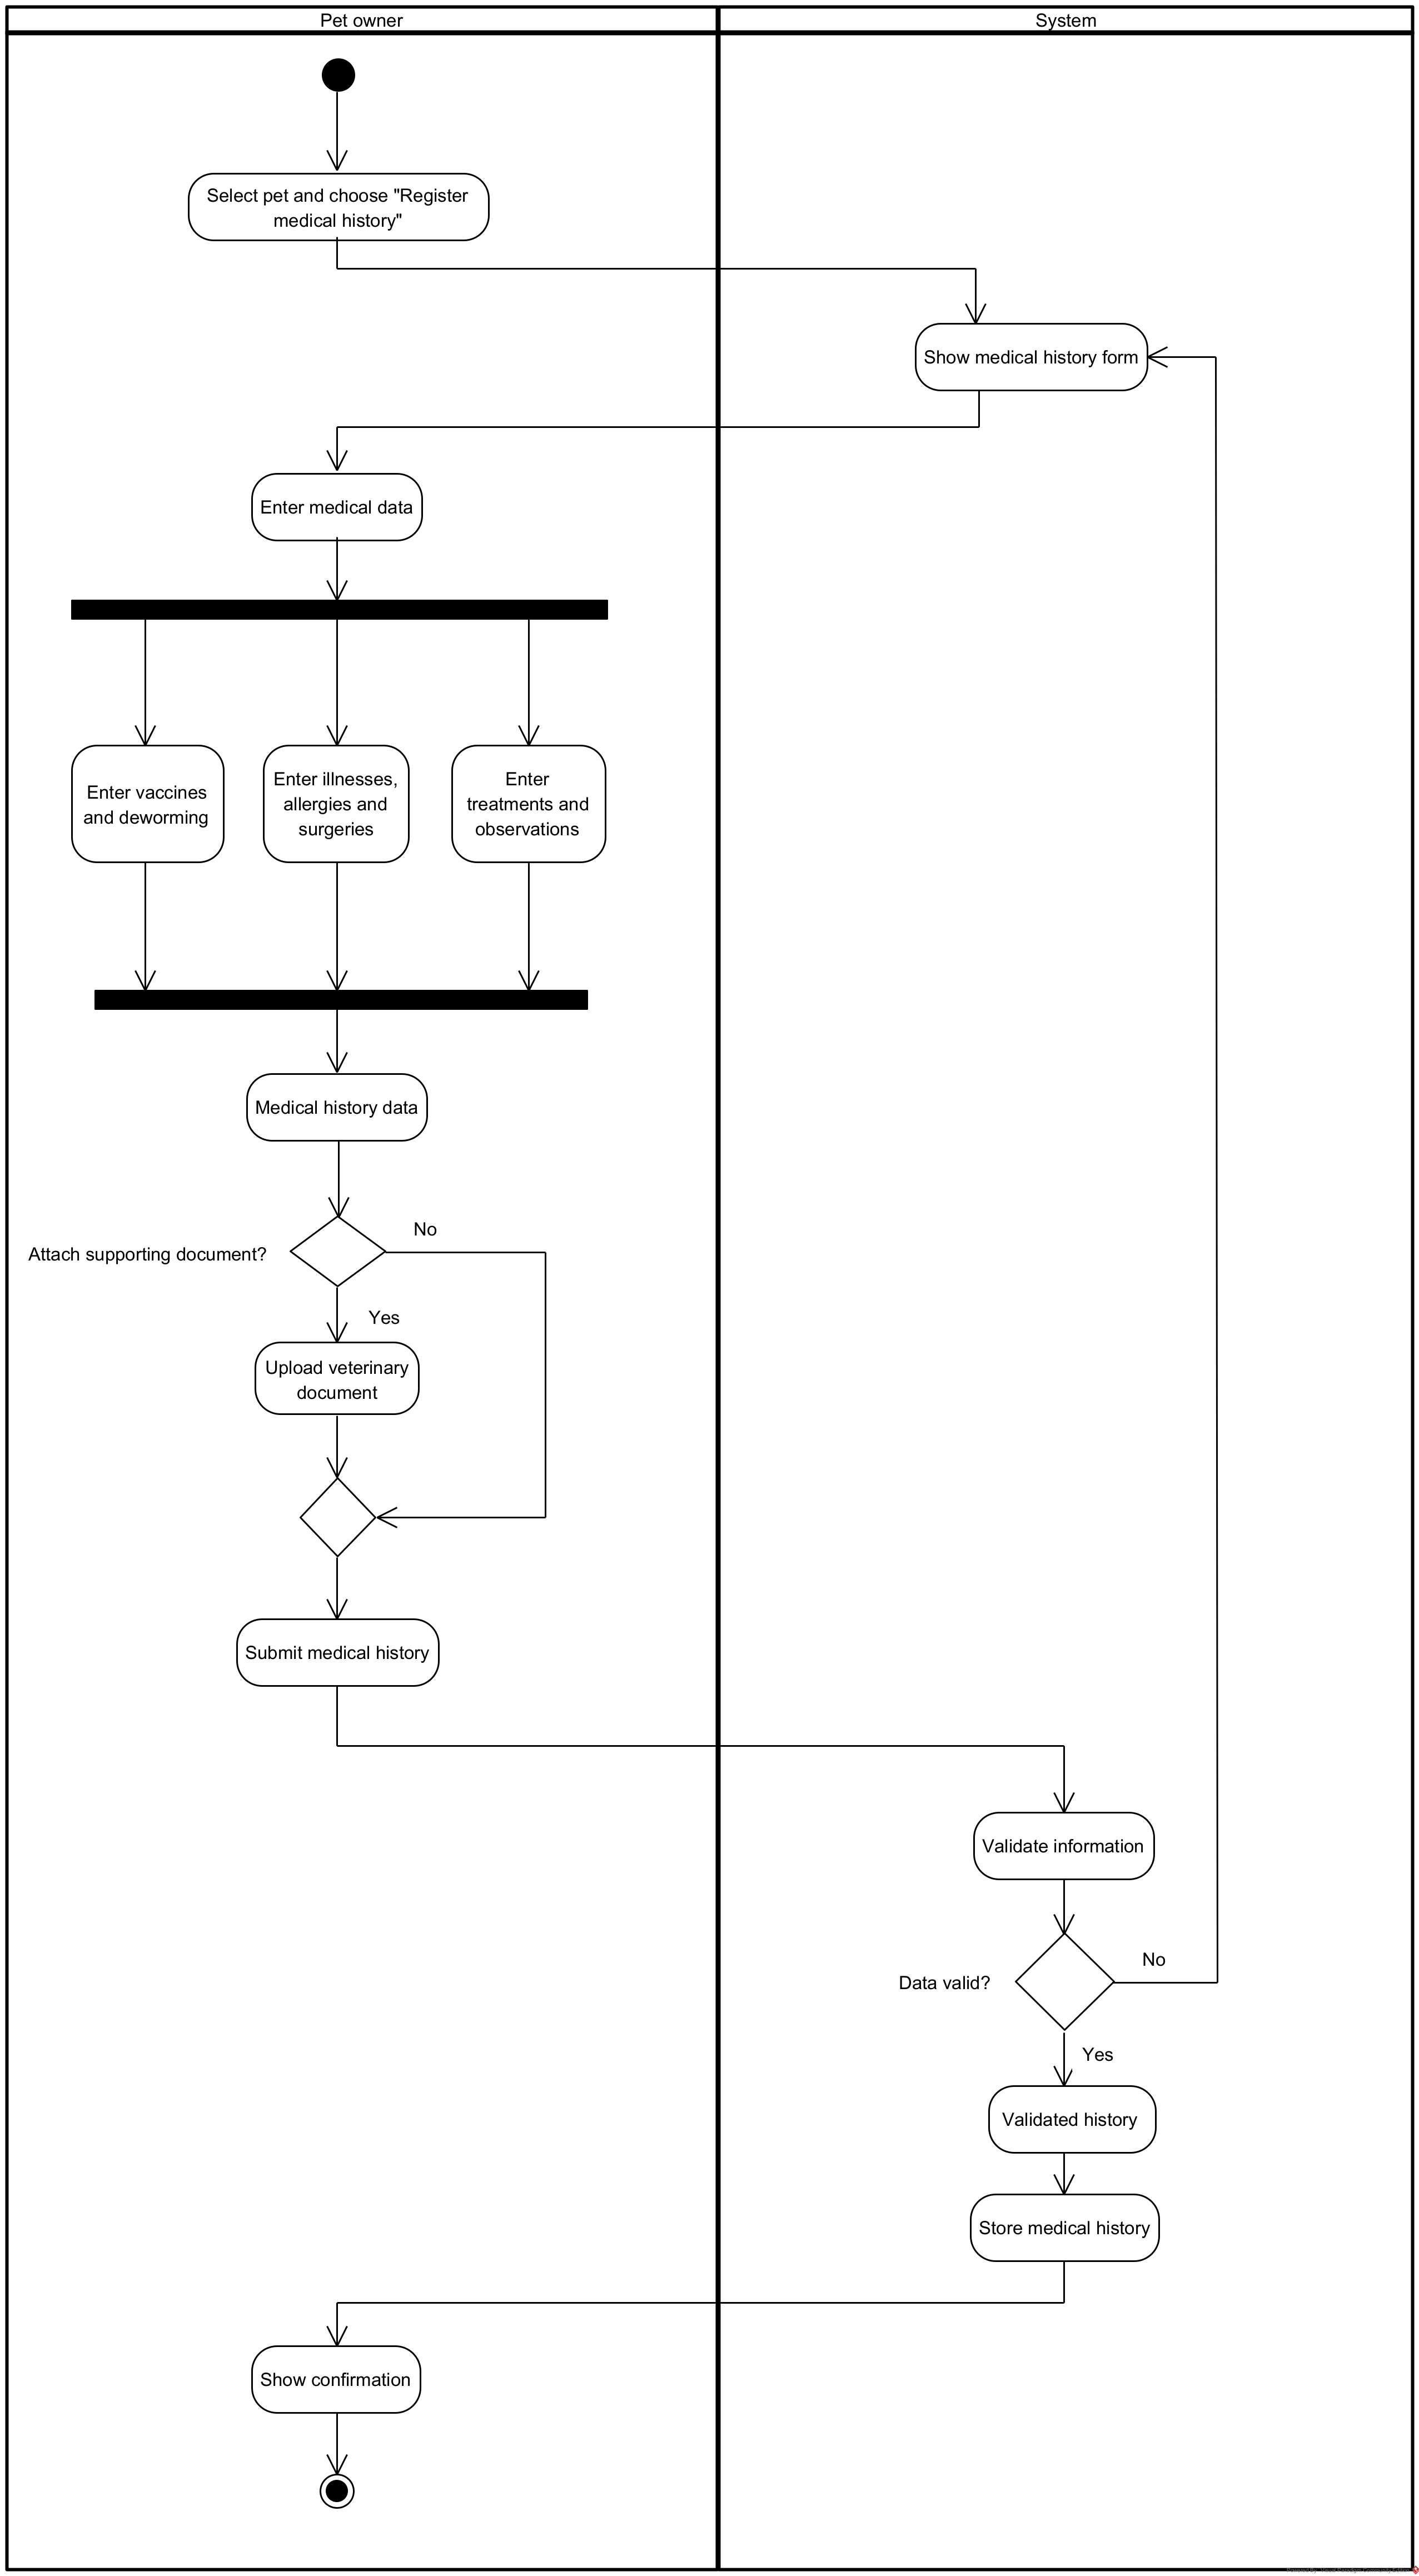
\includegraphics[width=0.5\textwidth]{DiagramaActividades_CU-02_MundiPets.png}
		\caption{Diagrama de actividades -- Registrar historial médico y antecedentes genéticos (CU-02).}
		\label{fig:act_cu02}
	\end{figure}
	
	Que ``Enter vaccines and deworming'', ``Enter illnesses...'' y ``Enter
	treatments...'' se ejecuten en una bifurcación paralela
	(\textit{fork/join}) y no en secuencia, según se observa en la
	Figura~\ref{fig:act_cu02}, revela que estas tres categorías de datos
	médicos son independientes entre sí y no existe un orden obligatorio de
	captura, permitiendo que el dueño complete primero la que tenga más a
	mano. Que ``Attach supporting document?'' sea una decisión opcional
	embebida dentro de este mismo caso de uso (y no delegada por completo al
	CU-03) muestra que subir el documento formal es una posibilidad
	conveniente durante el registro, aunque el CU-03 exista como flujo
	independiente para hacerlo después.
	
	\subsubsection{Cargar documento veterinario y carnet de vacunación (CU-03)}
	
	\begin{figure}[H]
		\centering
		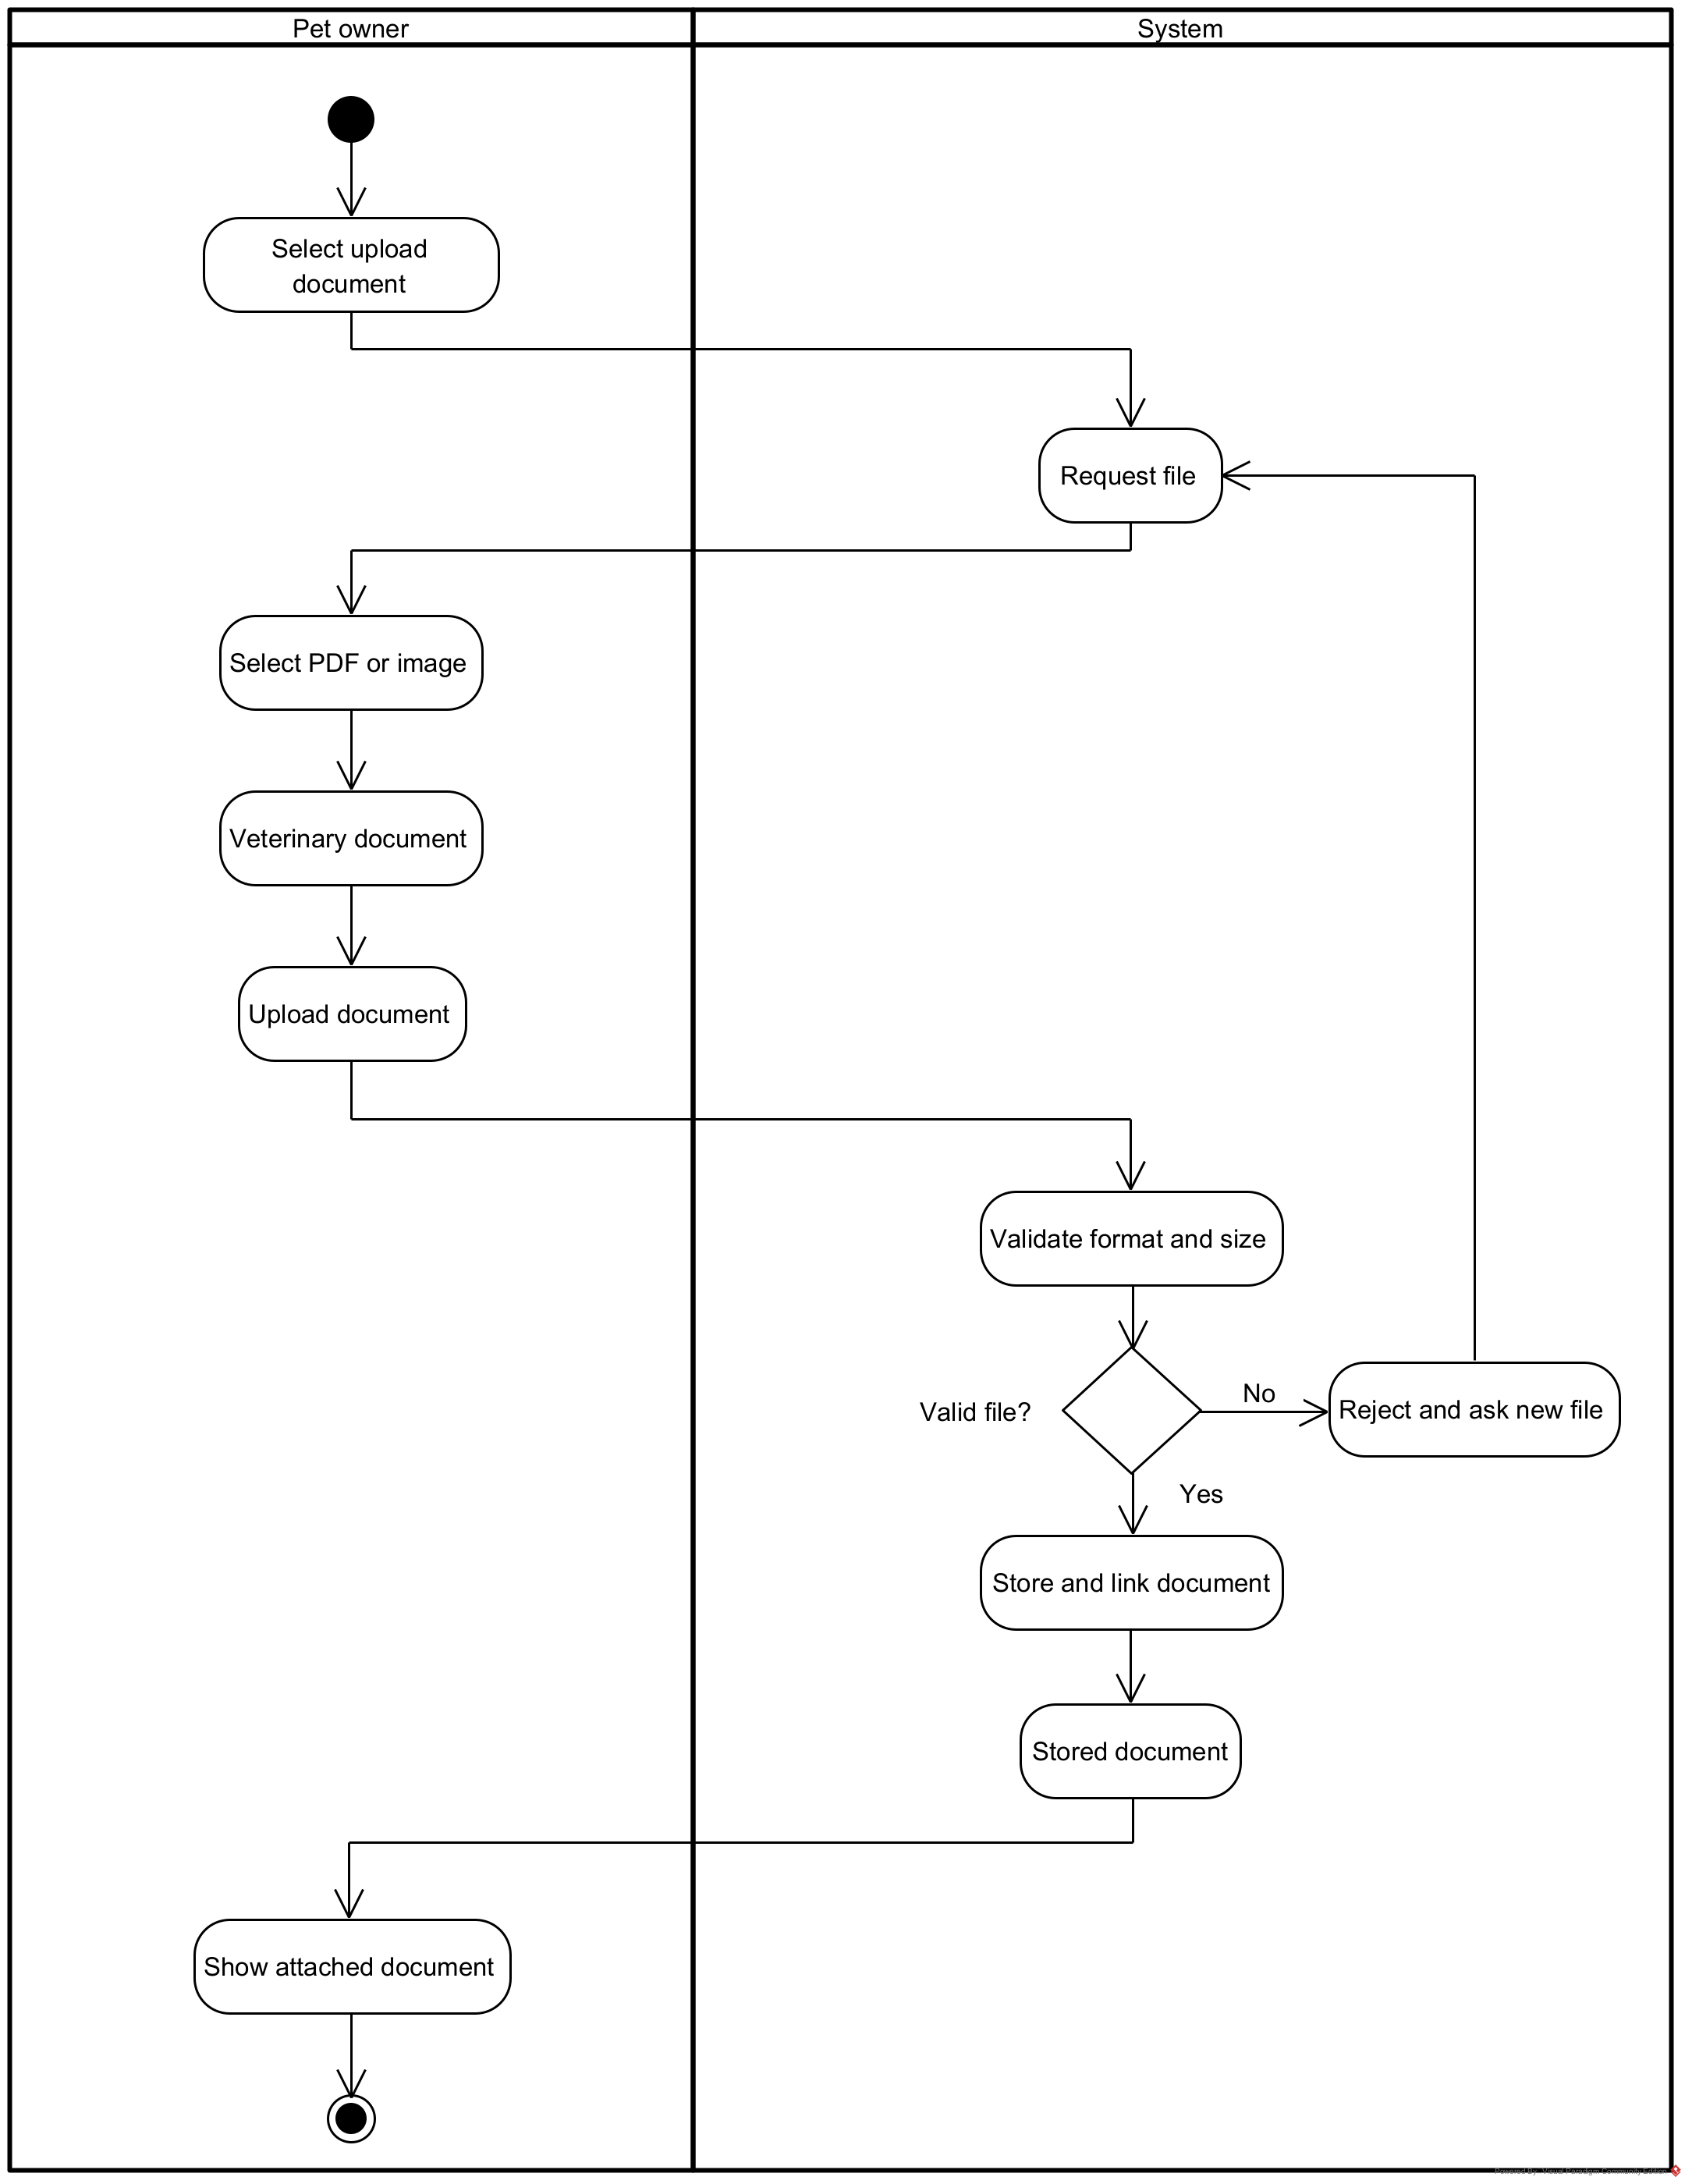
\includegraphics[width=0.55\textwidth]{DiagramaActividades_CU-03_MundiPets.png}
		\caption{Diagrama de actividades -- Cargar documento veterinario y carnet de vacunación (CU-03).}
		\label{fig:act_cu03}
	\end{figure}
	
	Que el rechazo del archivo (``Reject and ask new file'') regrese al nodo
	``Request file'' (y no obligue a reiniciar todo el caso de uso desde
	``Select upload document''), tal como se ve en la Figura~\ref{fig:act_cu03},
	revela que el sistema minimiza la fricción ante un archivo inválido,
	permitiendo reintentar solo el paso de selección del archivo sin perder
	el contexto de a qué historial médico pertenece.
	
	\subsubsection{Publicar mascota en adopción (CU-04)}
	
	\begin{figure}[H]
		\centering
		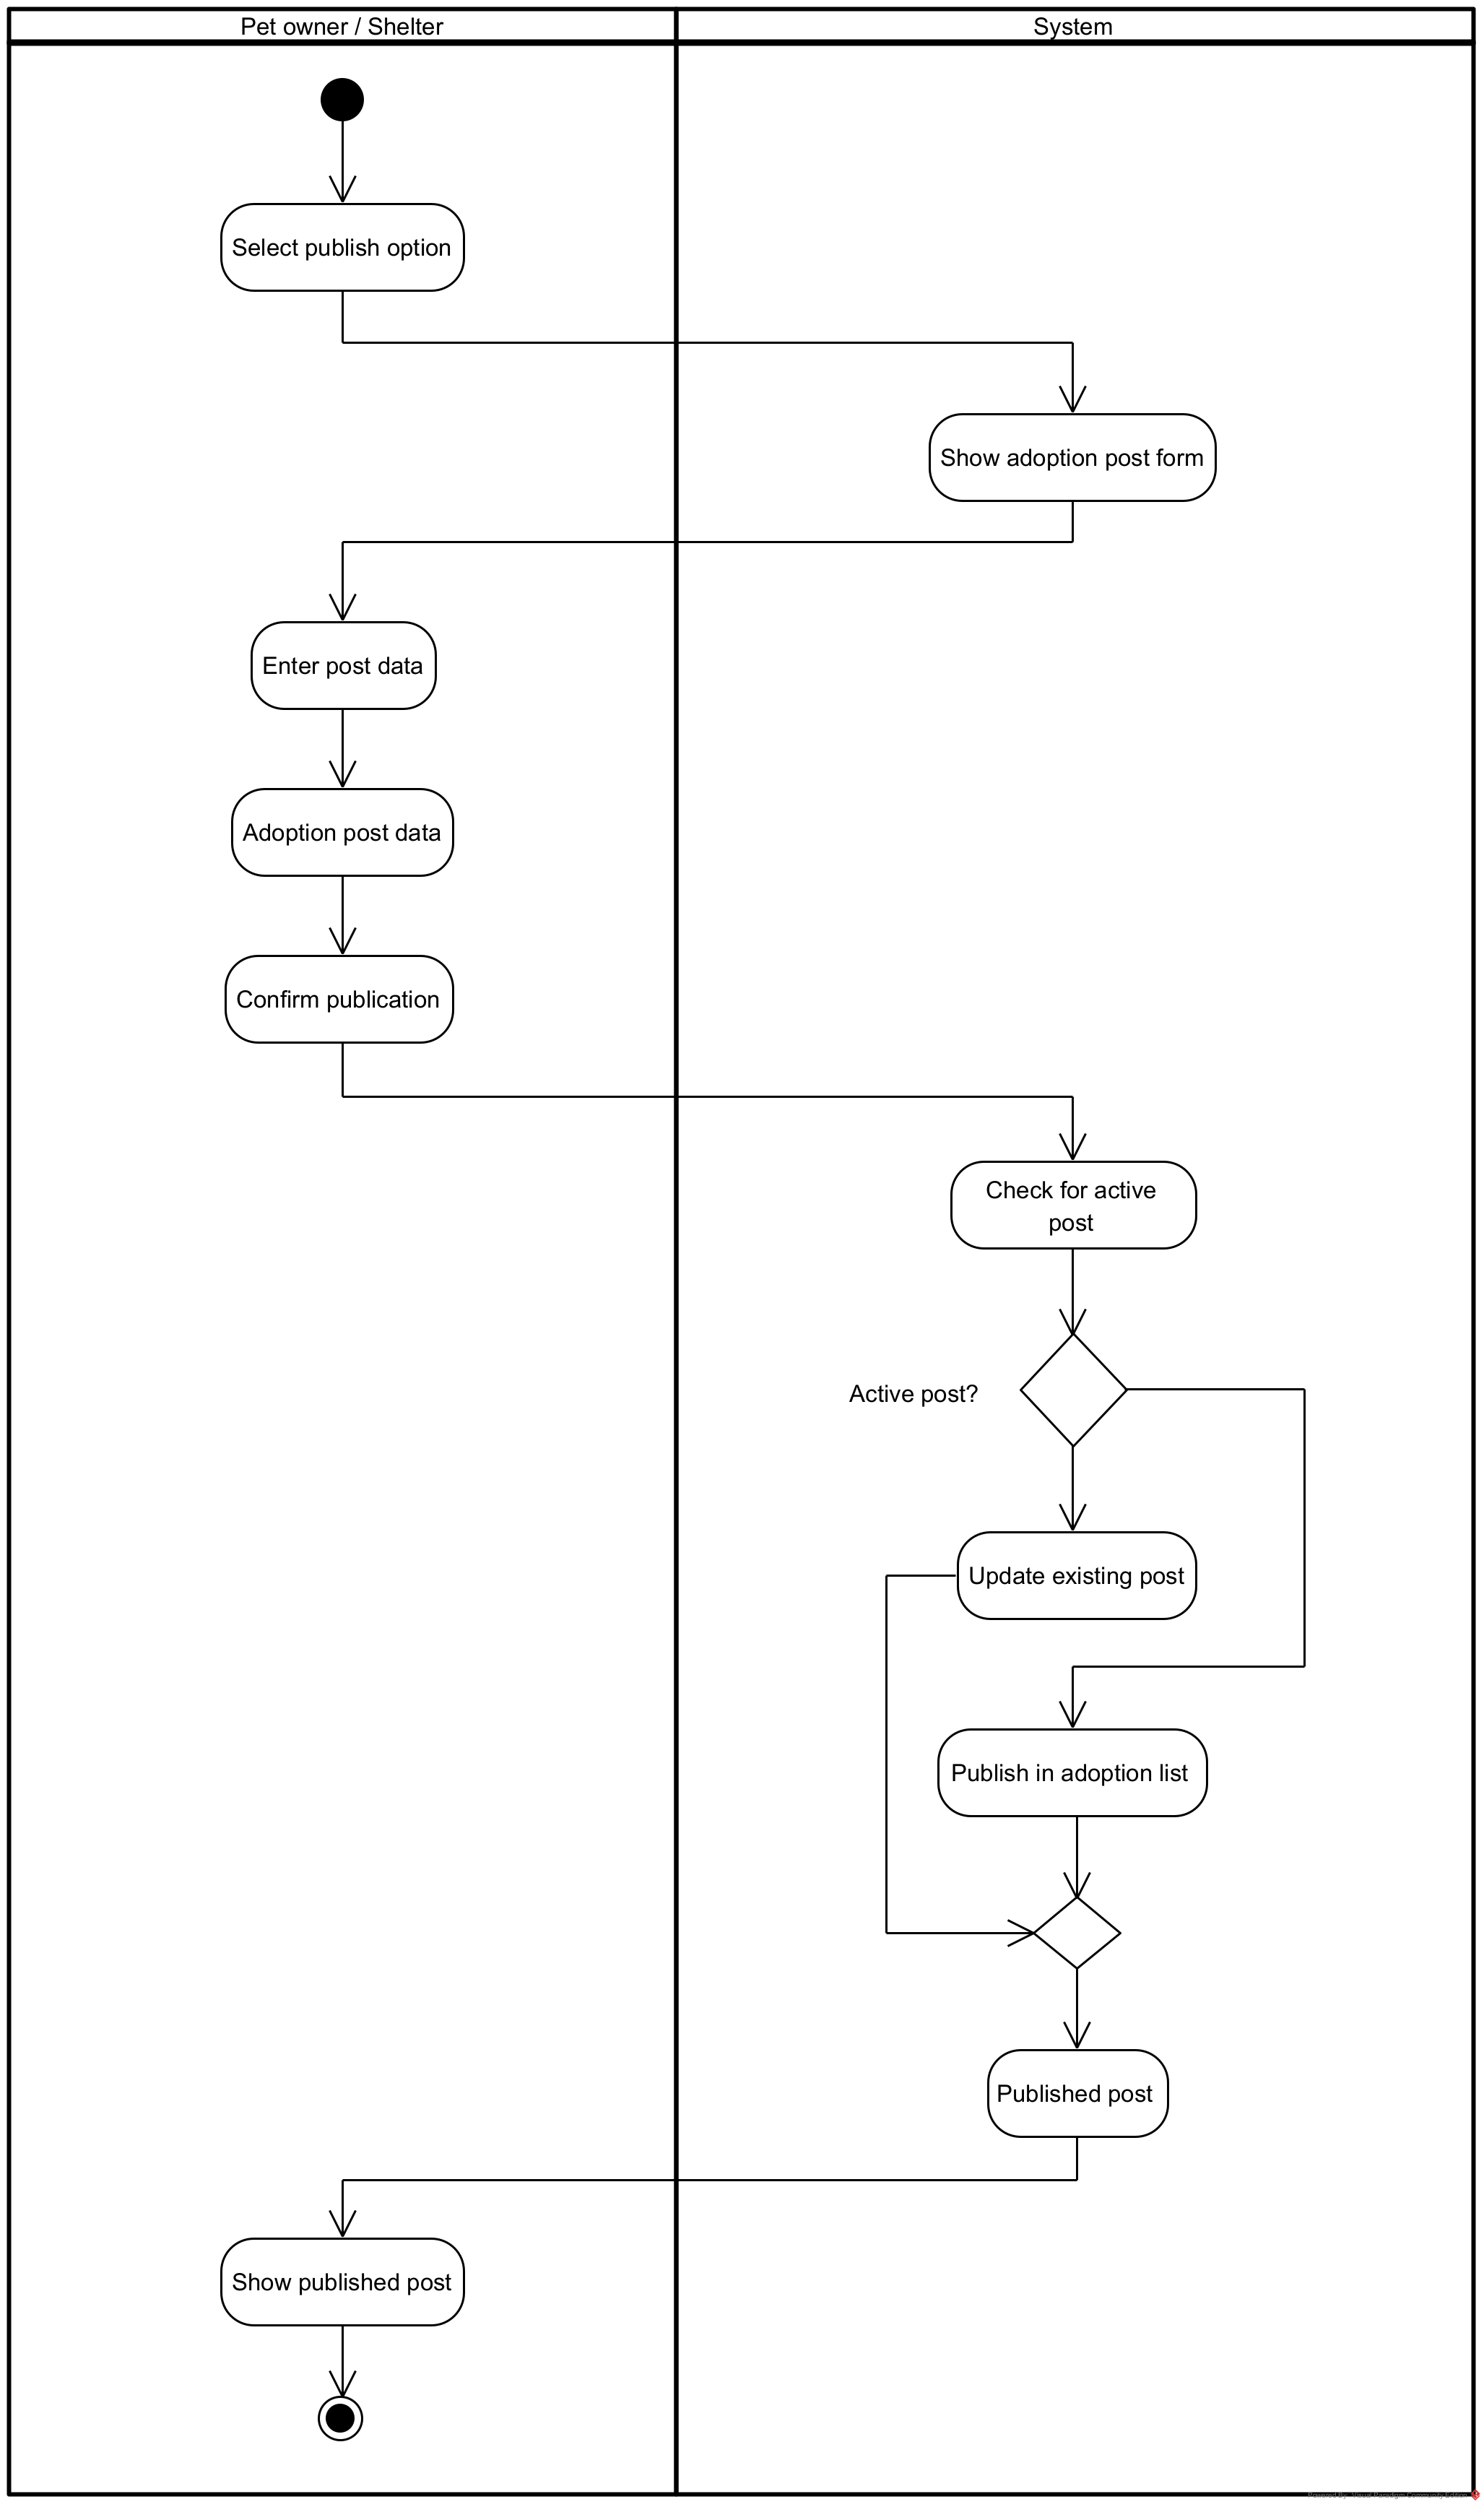
\includegraphics[width=0.5\textwidth]{DiagramaActividades_CU-04_MundiPets.png}
		\caption{Diagrama de actividades -- Publicar mascota en adopción (CU-04).}
		\label{fig:act_cu04}
	\end{figure}
	
	Que la decisión ``Active post?'' determine si se ejecuta ``Update
	existing post'' antes de fusionar el flujo hacia ``Publish in adoption
	list'' (ambas ramas convergen al mismo paso de publicación), como se
	observa en la Figura~\ref{fig:act_cu04}, revela que, exista o no una
	publicación previa, el resultado final es siempre una sola publicación
	activa vigente: el sistema absorbe la lógica de duplicados de forma
	transparente para el usuario, que solo ve el resultado publicado, sin
	pasos adicionales visibles según el caso.
	
	\subsubsection{Publicar mascota para cruza y gestionar solicitud (CU-05)}
	
	\begin{figure}[H]
		\centering
		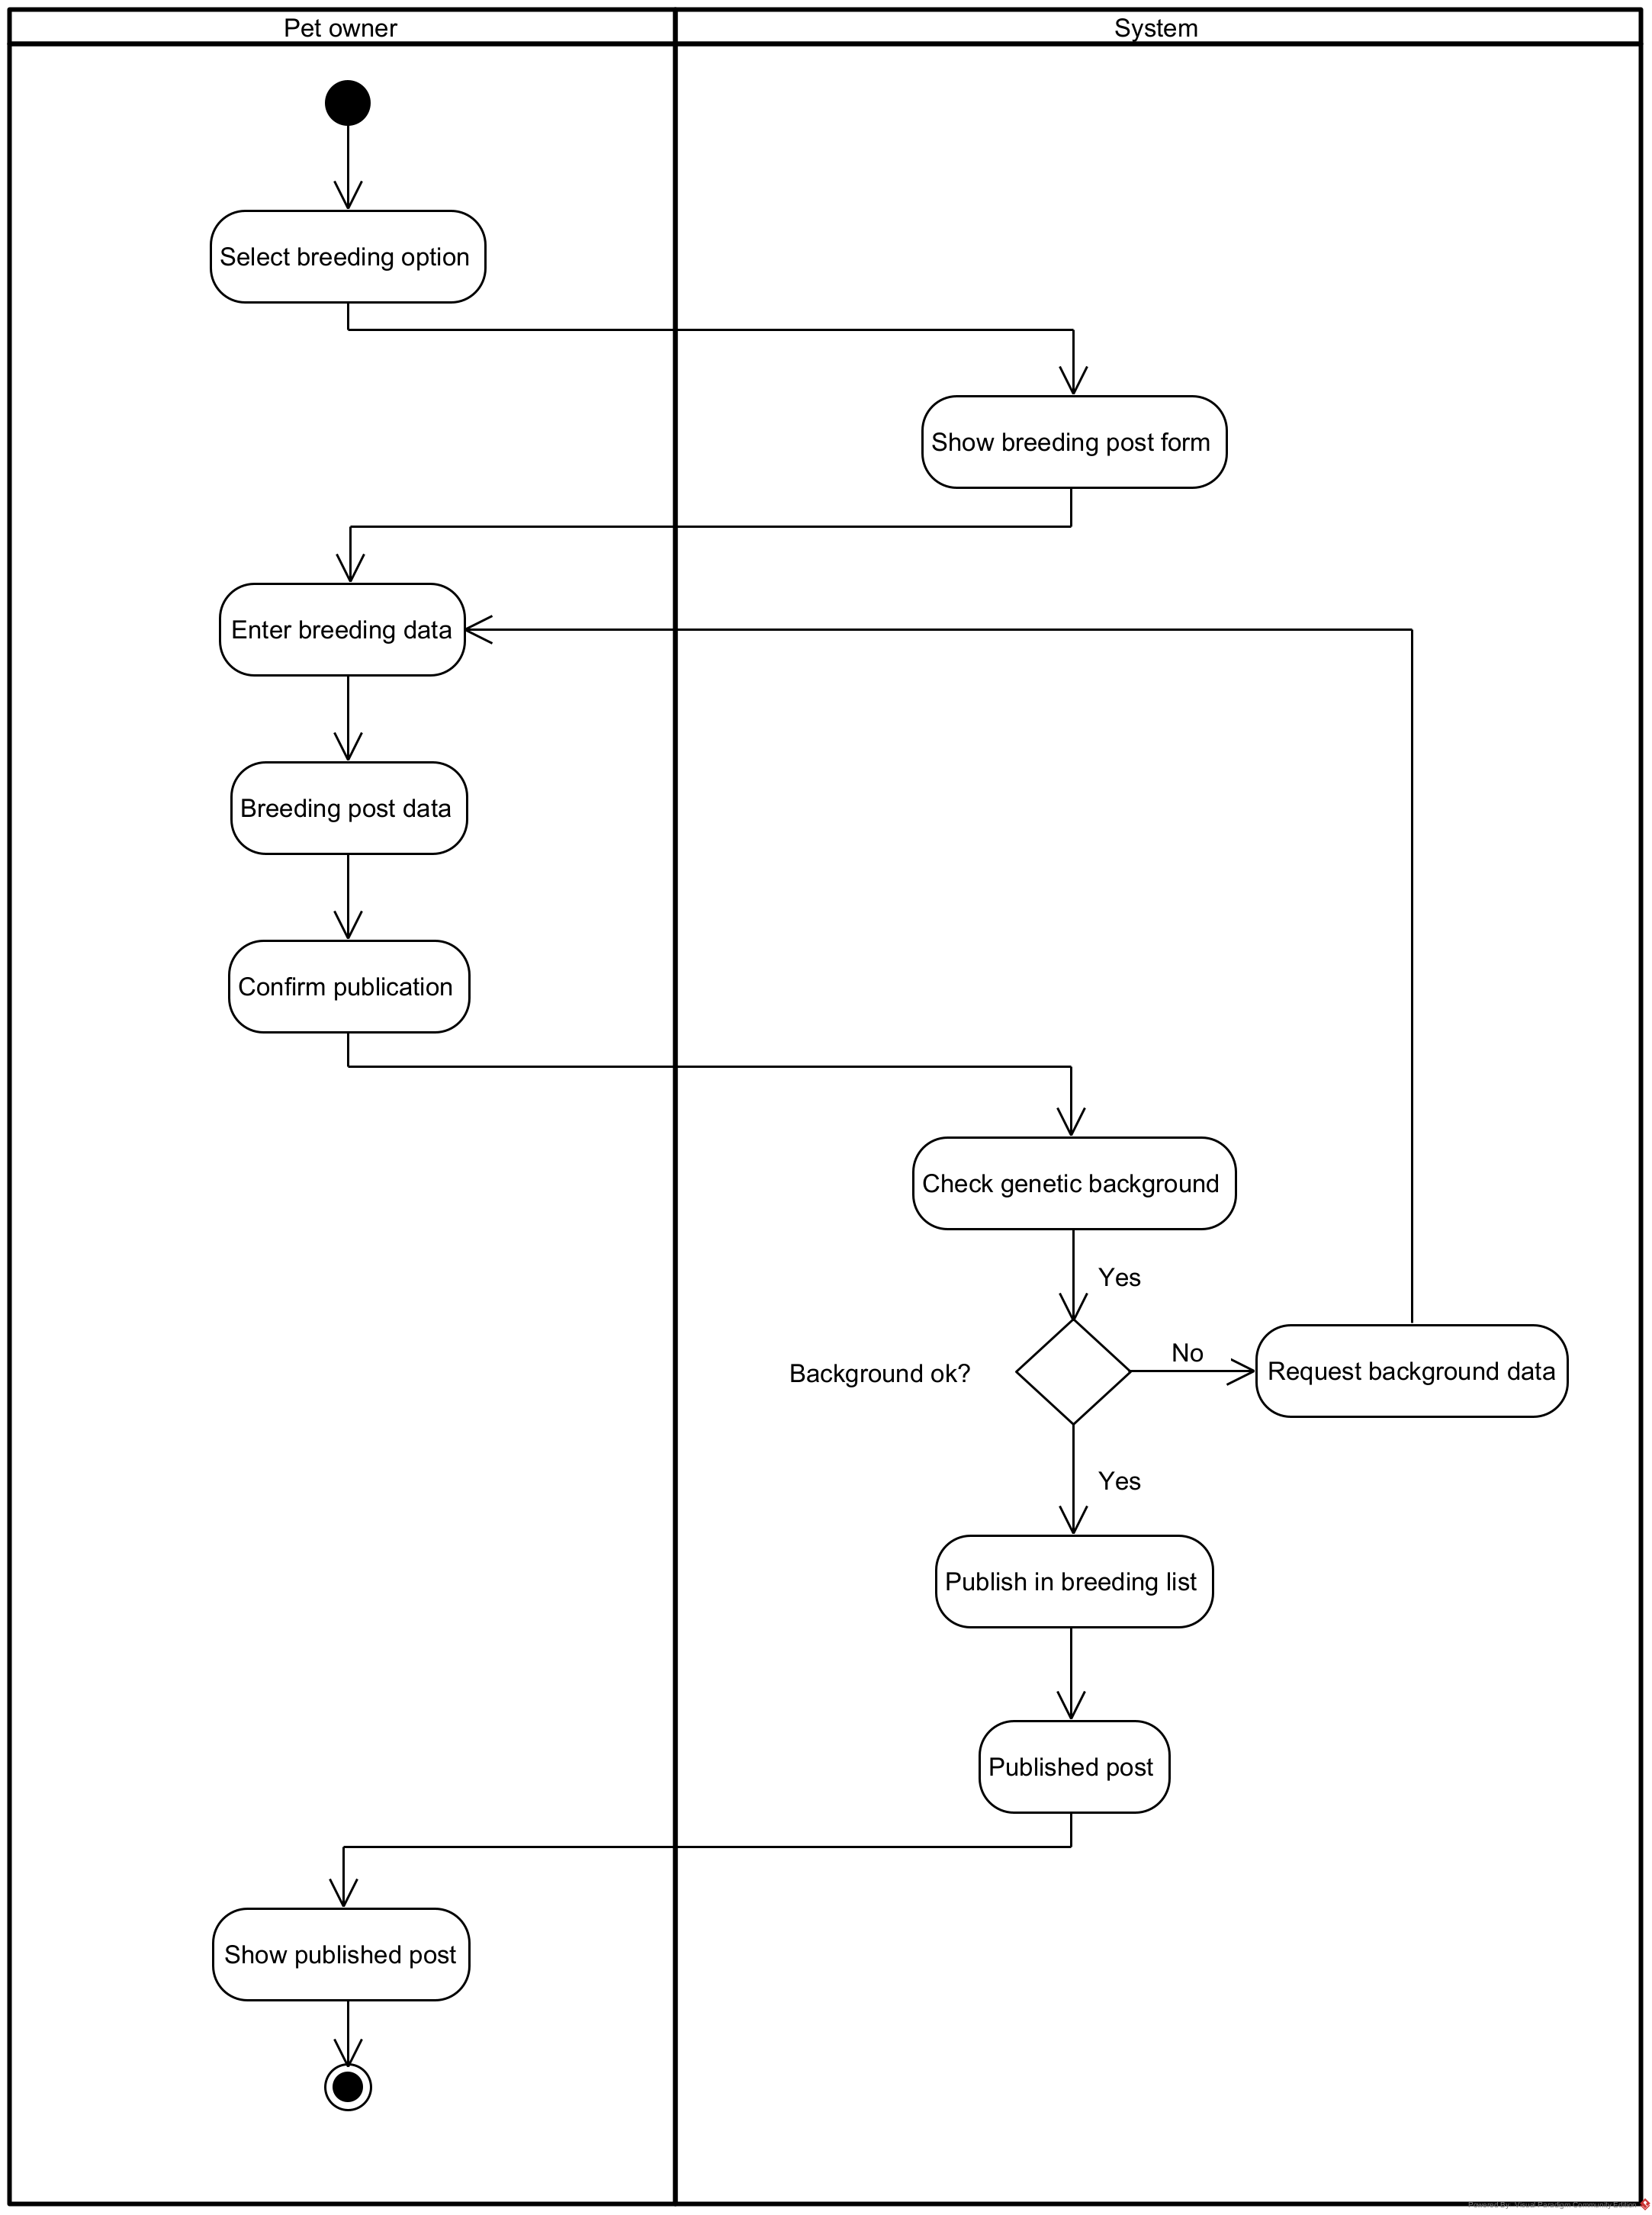
\includegraphics[width=0.95\textwidth]{DiagramaActividades_CU-05_MundiPets.png}
		\caption{Diagrama de actividades -- Publicar mascota para cruza y gestionar solicitud (CU-05).}
		\label{fig:act_cu05}
	\end{figure}
	
	Que ``Background ok?'' con salida ``No'' regrese específicamente a
	``Enter breeding data'' (y no a ``Show breeding post form'' como en
	otros flujos), tal como se ve en la Figura~\ref{fig:act_cu05}, revela que
	el sistema no permite publicar sin importar cuántas veces se lo intente
	si falta el antecedente genético: el dueño queda atrapado en un ciclo de
	corrección hasta cumplir este requisito no negociable, reafirmando
	visualmente lo mismo que ya mostró el diagrama de secuencia CU-05
	(Figura~\ref{fig:sec_cu05}): la trazabilidad genética es condición dura,
	no sugerencia.
	
	\subsubsection{Configurar privacidad médica (CU-06)}
	
	\begin{figure}[H]
		\centering
		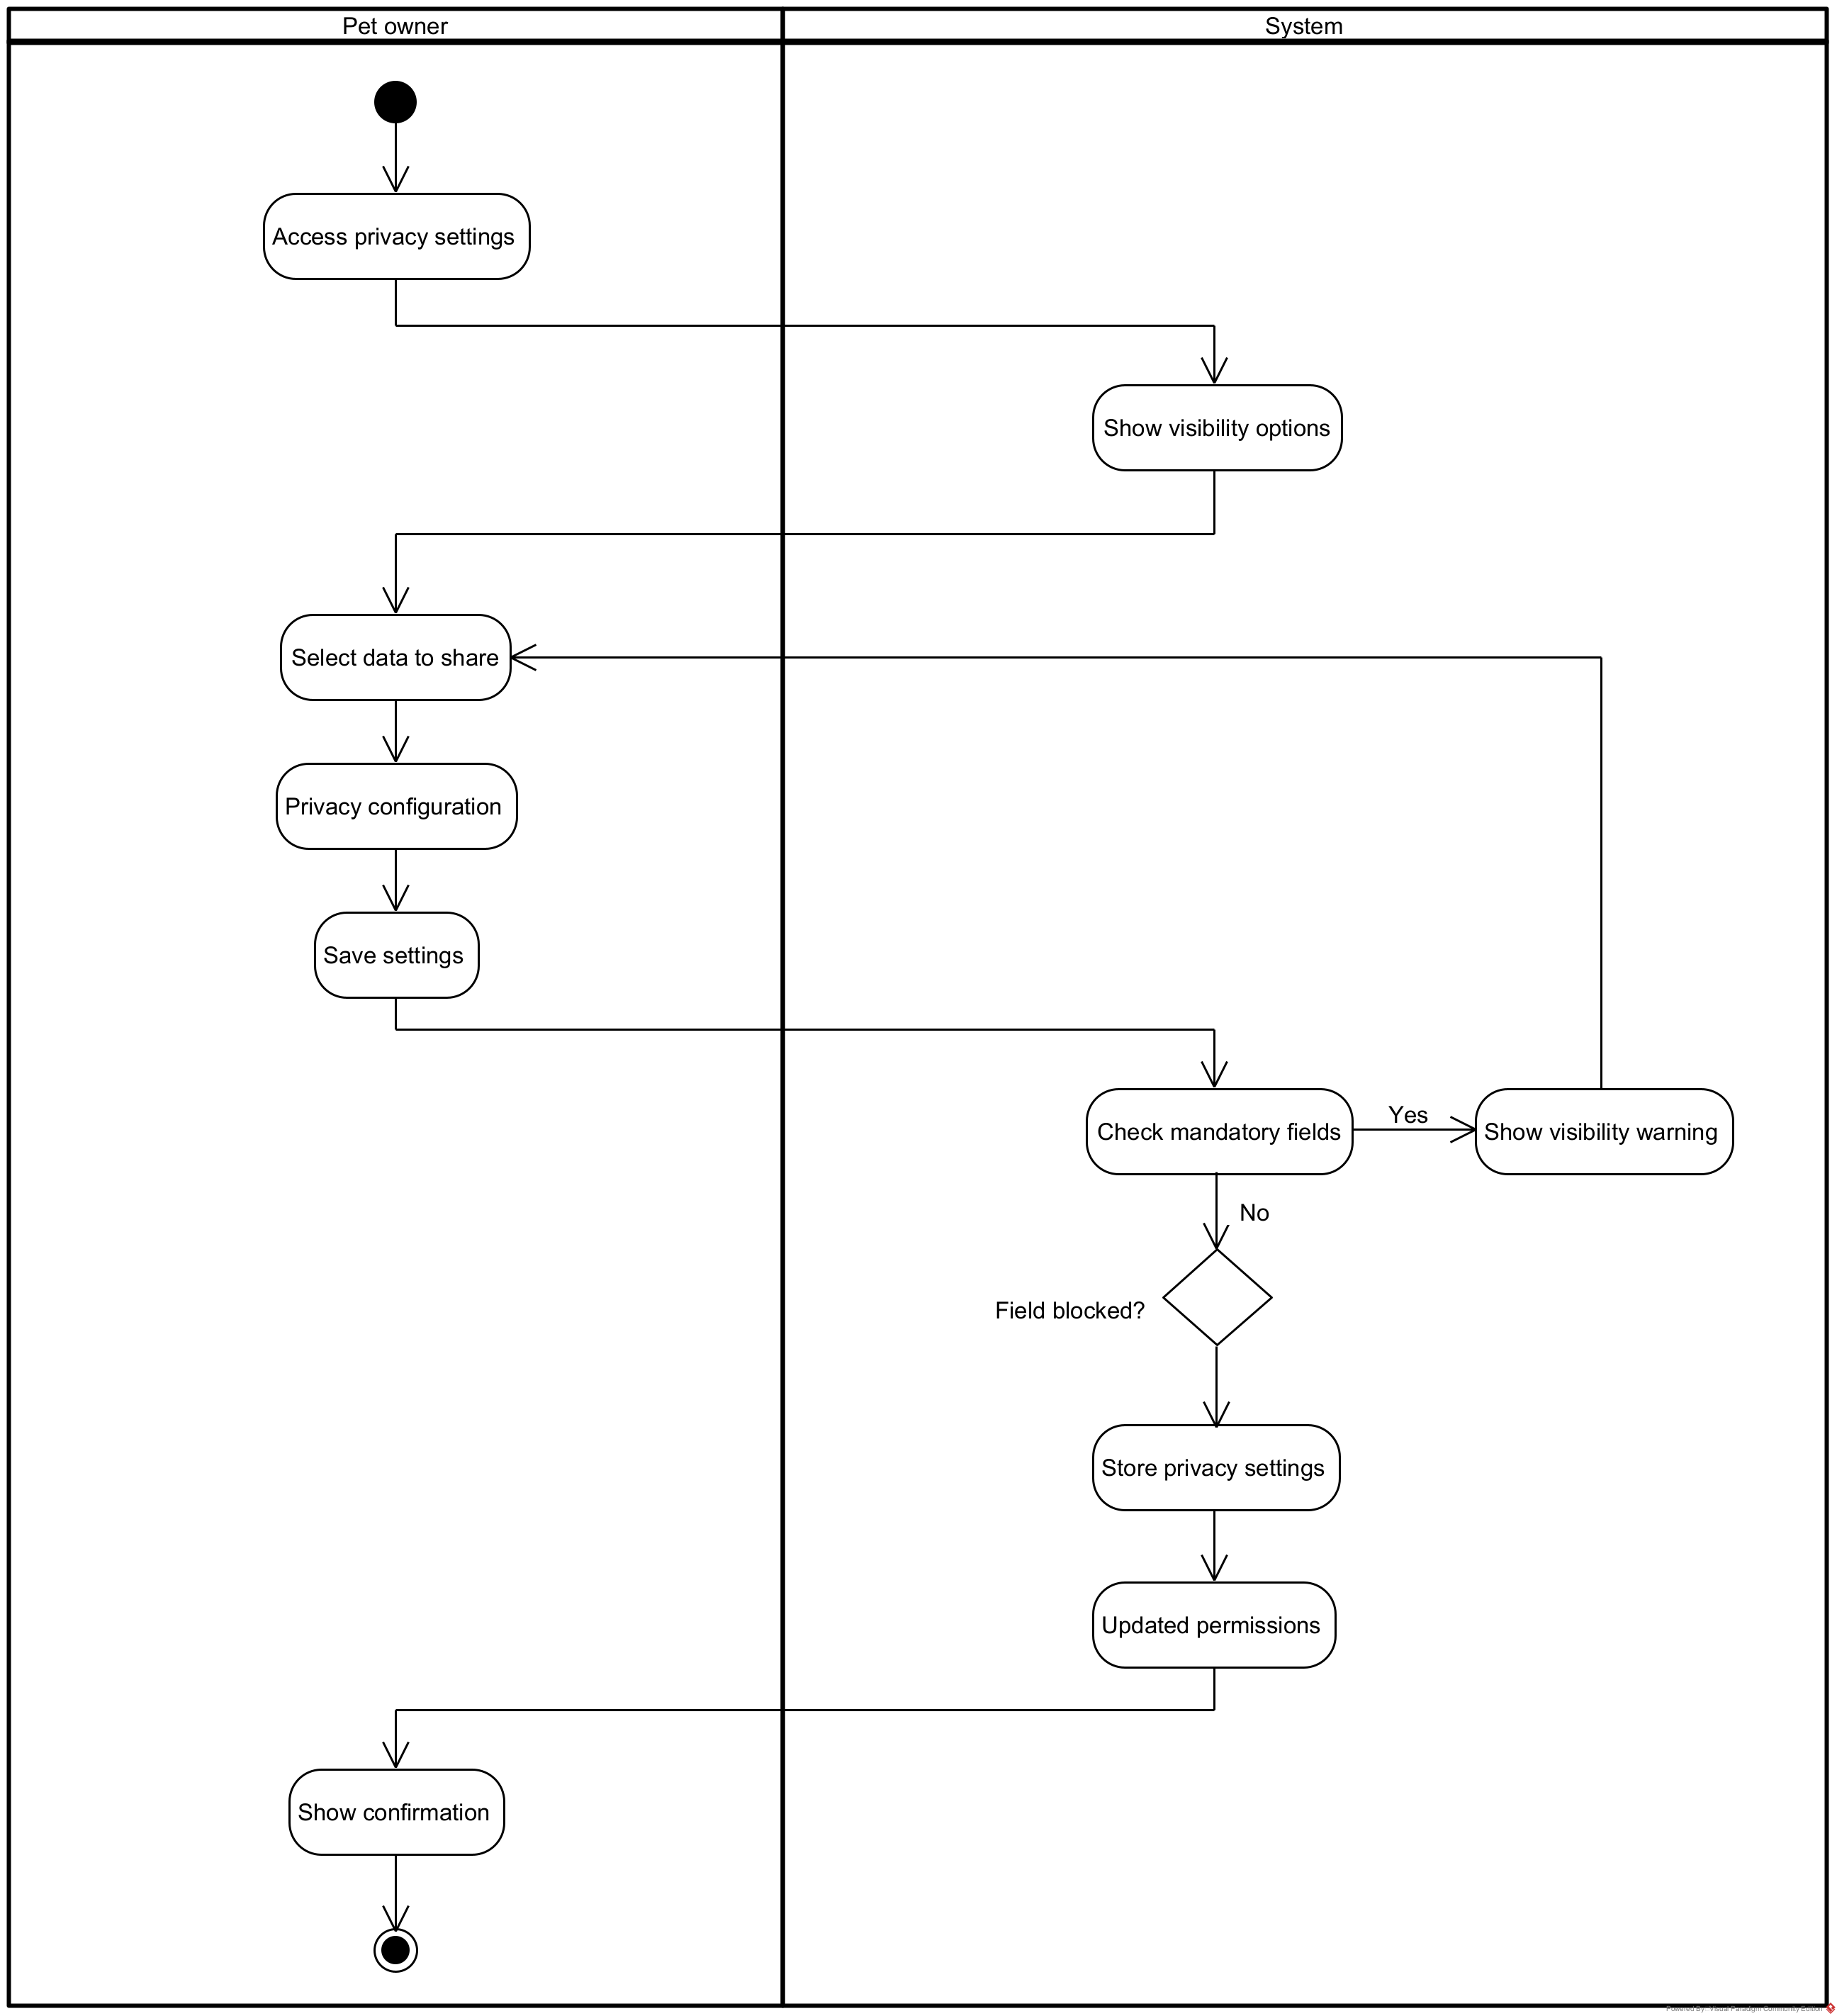
\includegraphics[width=0.95\textwidth]{DiagramaActividades_CU-06_MundiPets.png}
		\caption{Diagrama de actividades -- Configurar privacidad médica (CU-06).}
		\label{fig:act_cu06}
	\end{figure}
	
	Que ``Check mandatory fields'' con salida ``Yes'' (campo bloqueado
	indebidamente) regrese a ``Select data to share'' mediante ``Show
	visibility warning'' (en vez de simplemente no guardar el cambio en
	silencio), como se ve en la Figura~\ref{fig:act_cu06}, revela que el
	sistema educa activamente al dueño sobre por qué su configuración fue
	rechazada, en lugar de aplicar un filtro invisible que ignore la
	instrucción del usuario sin explicación.
	
	\subsubsection{Gestionar proceso de adopción (CU-07)}
	
	\begin{figure}[H]
		\centering
		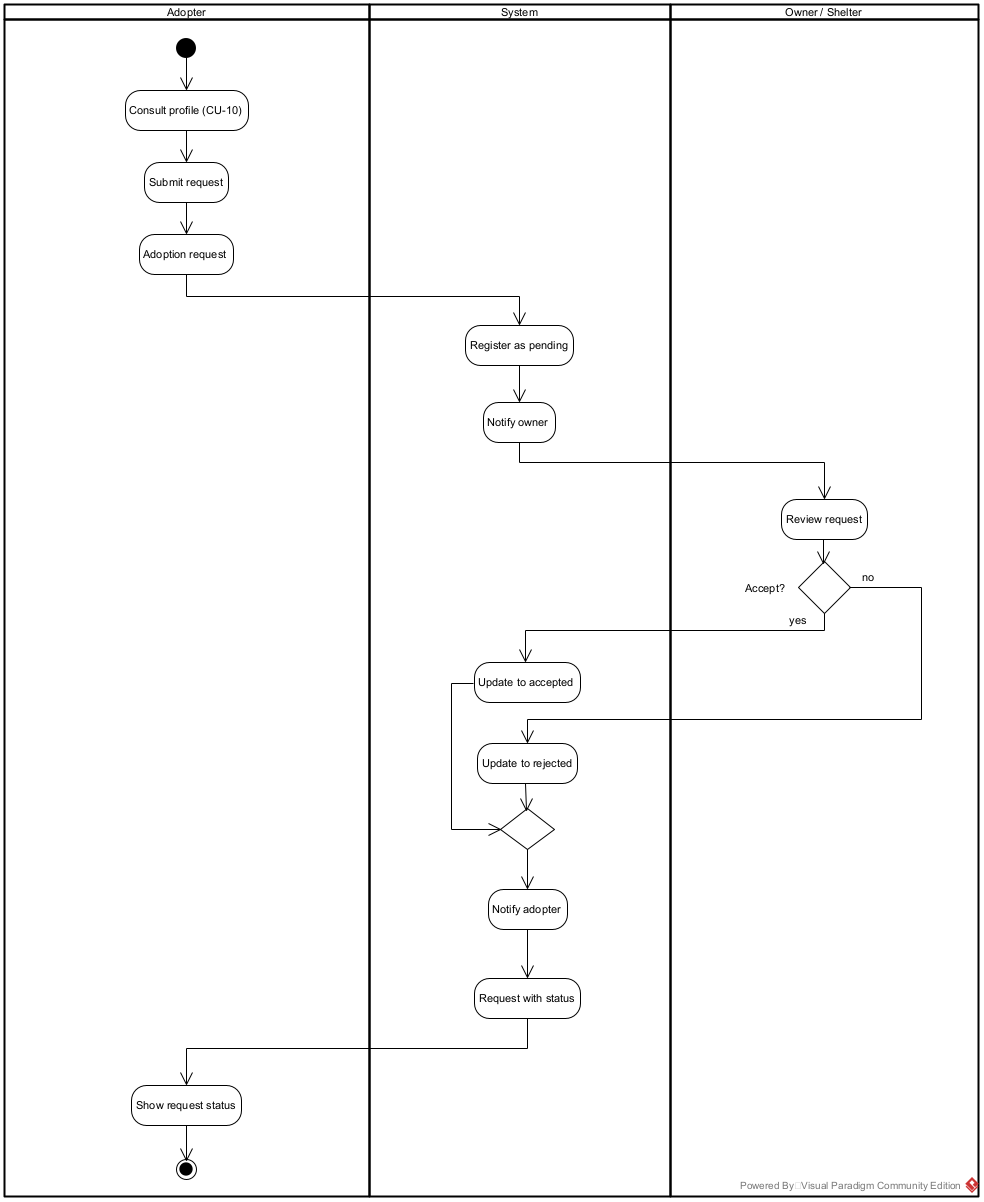
\includegraphics[width=0.85\textwidth]{DiagramaActividades_CU-07_MundiPets.png}
		\caption{Diagrama de actividades -- Gestionar proceso de adopción (CU-07).}
		\label{fig:act_cu07}
	\end{figure}
	
	Que exista un carril separado ``Owner / Shelter'' distinto del carril
	``System'' para la actividad ``Review request'', tal como se ve en la
	Figura~\ref{fig:act_cu07}, revela que la decisión de aceptar o rechazar
	una solicitud es exclusivamente humana y deliberada, sin ningún paso
	automatizado de aprobación: el sistema solo gestiona el registro y la
	notificación, nunca decide en nombre del dueño.
	
	\subsubsection{Gestionar comunicación entre usuarios (CU-08)}
	
	\begin{figure}[H]
		\centering
		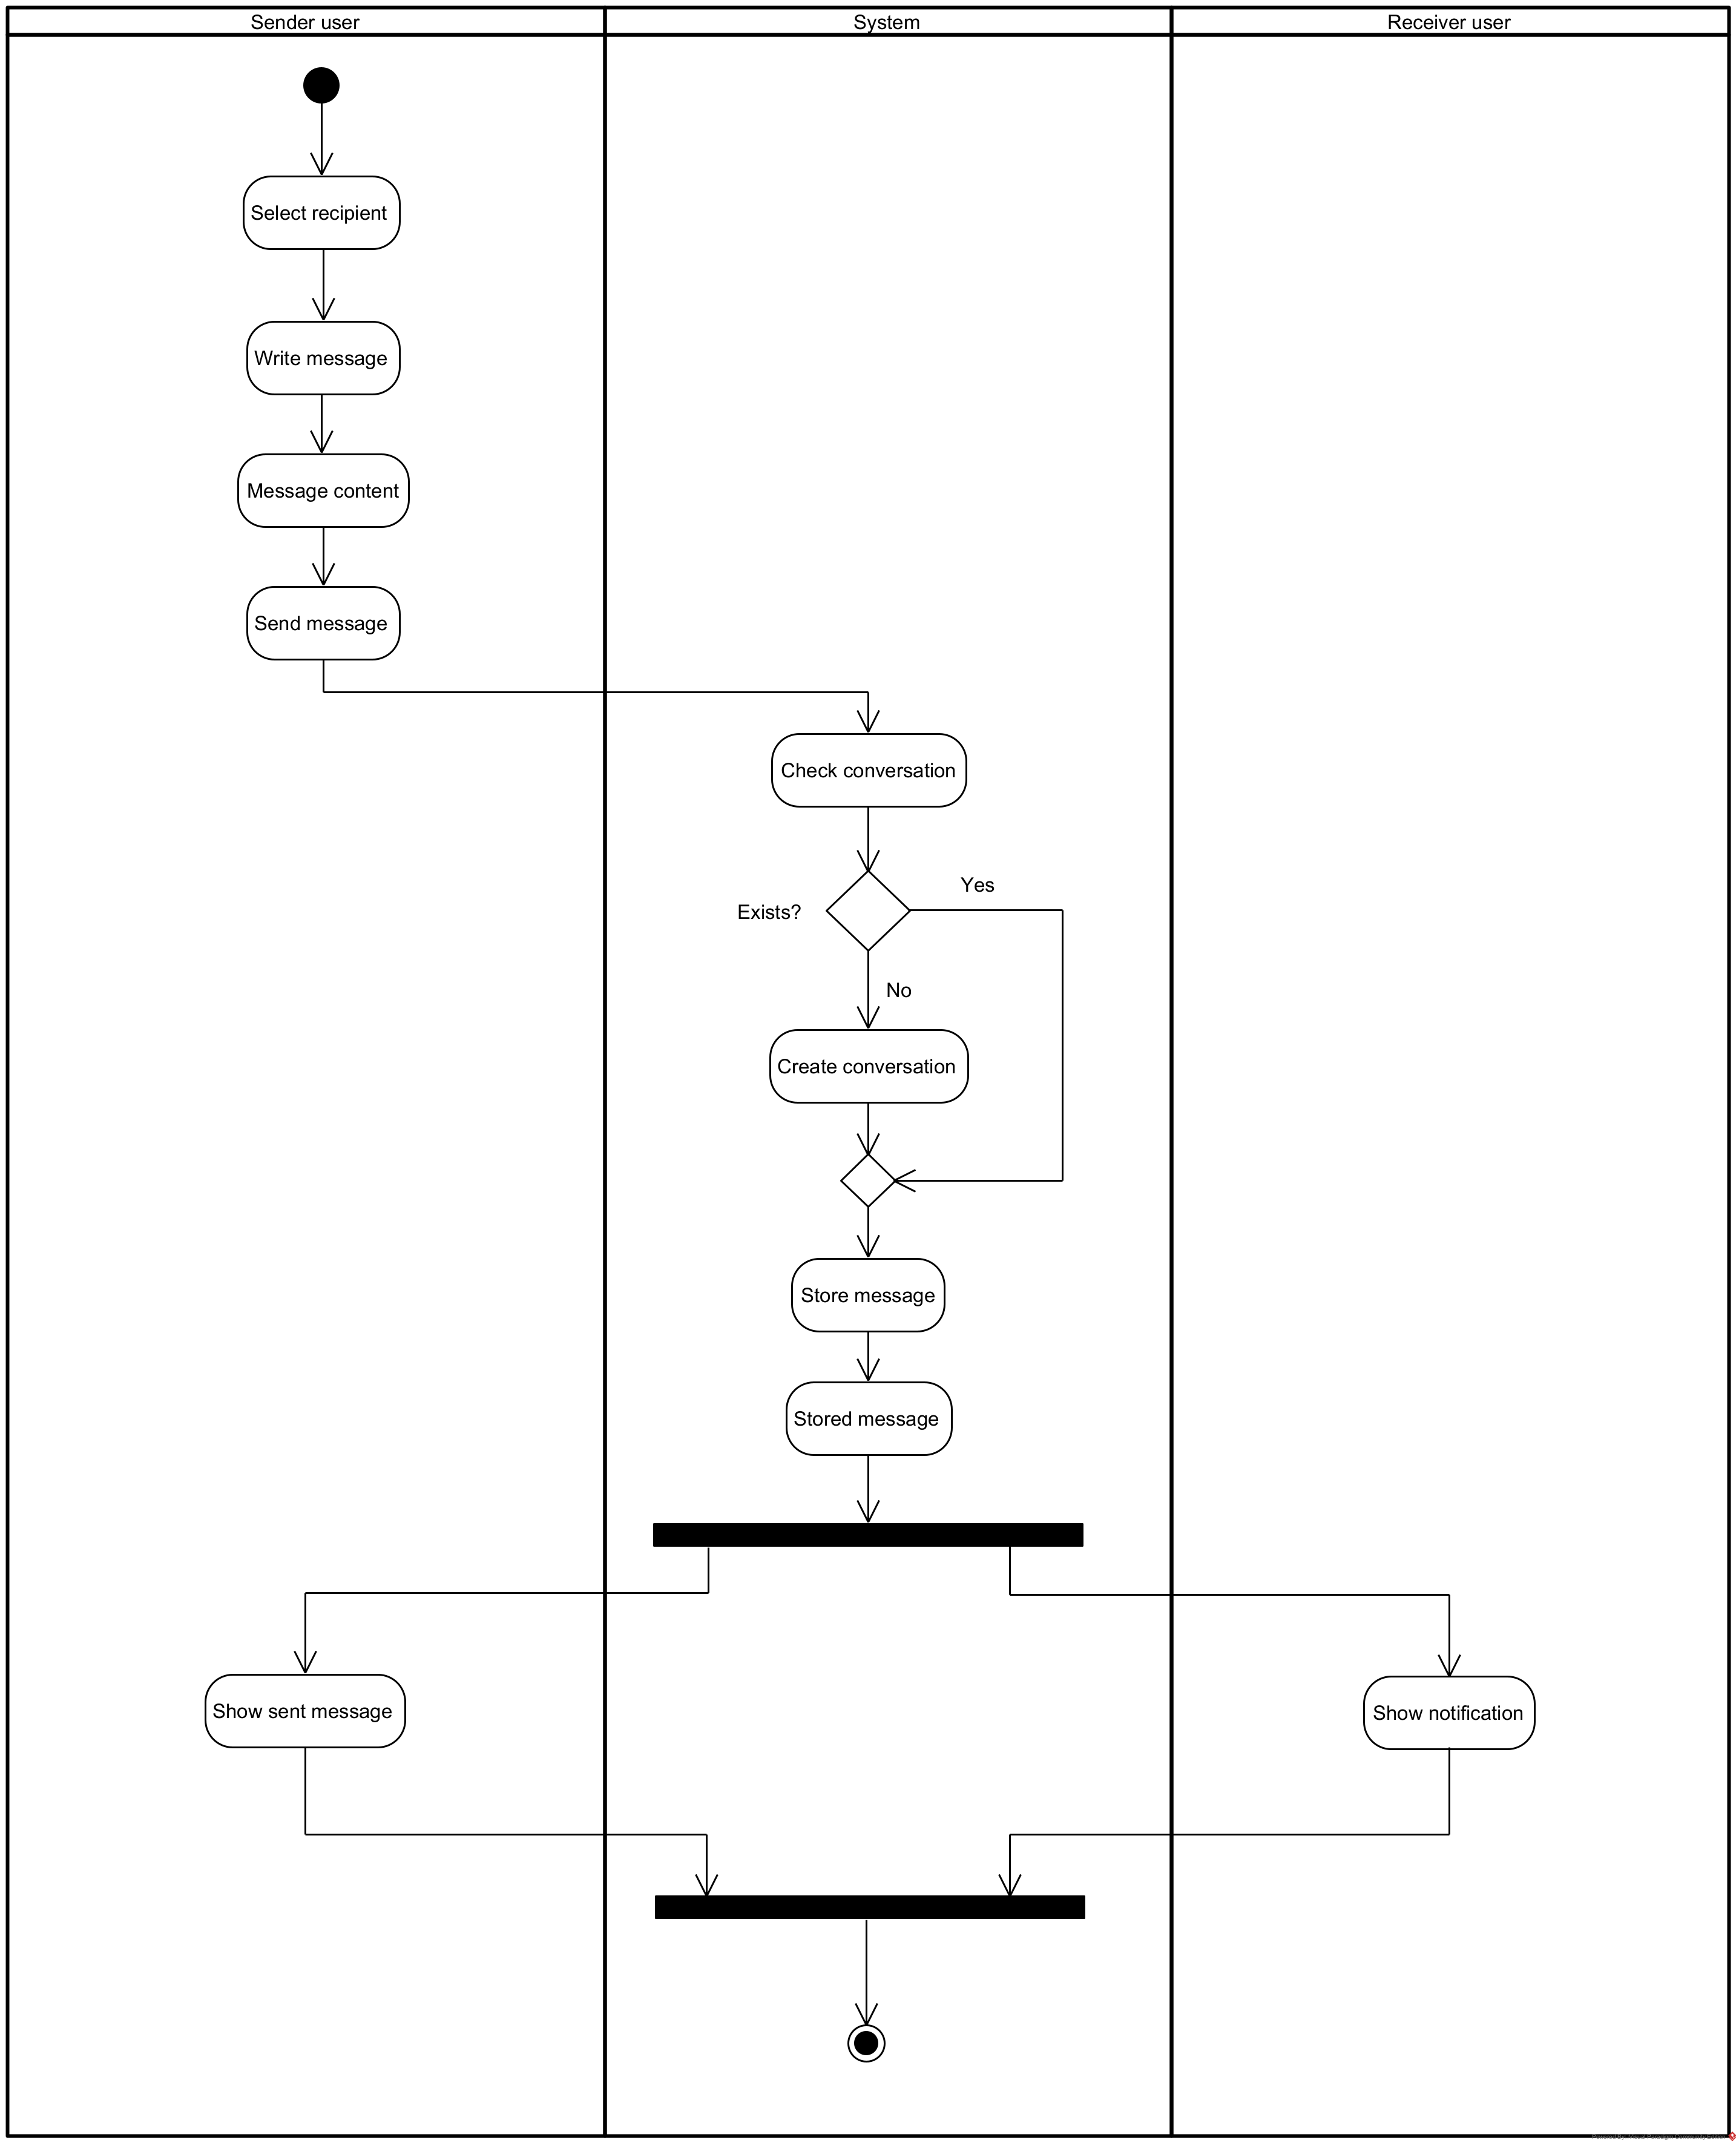
\includegraphics[width=0.95\textwidth]{DiagramaActividades_CU-08_MundiPets.png}
		\caption{Diagrama de actividades -- Gestionar comunicación entre usuarios (CU-08).}
		\label{fig:act_cu08}
	\end{figure}
	
	Que el diagrama cierre con una bifurcación (\textit{fork}) que ejecuta en
	paralelo ``Show sent message'' (carril \textit{Sender}) y ``Show
	notification'' (carril \textit{Receiver}), como se observa en la
	Figura~\ref{fig:act_cu08}, revela que el sistema trata la confirmación
	del emisor y la alerta del receptor como dos efectos simultáneos e
	independientes de un mismo evento de guardado, y no como una cadena
	secuencial donde uno depende del otro.
	
	\subsubsection{Validar información médica (CU-09)}
	
	\begin{figure}[H]
		\centering
		
\includegraphics[width=0.5\textwidth]{DiagramaActividades_CU-09_MundiPets.png}
		\caption{Diagrama de actividades -- Validar información médica (CU-09).}
		\label{fig:act_cu09}
	\end{figure}
	
	Que el flujo de rechazo (``Reject validation'') no reingrese al ciclo de
	revisión sino que termine directamente en su propio nodo final (``Show
	rejection''), tal como se ve en la Figura~\ref{fig:act_cu09}, revela que,
	a diferencia del CU-05 o CU-06, esta actividad no fuerza una corrección
	inmediata: el veterinario simplemente cierra el caso como rechazado y es
	el dueño quien deberá iniciar un nuevo ciclo de validación por separado,
	coherente con la máquina de estados de Verificación de Documentos
	(Figura~\ref{fig:me_verificacion}).
	
	\subsubsection{Consultar perfil médico (CU-10)}
	
	\begin{figure}[H]
		\centering
		
\includegraphics[width=0.75\textwidth]{DiagramaActividades_CU-10_MundiPets.png}
		\caption{Diagrama de actividades -- Consultar perfil médico (CU-10).}
		\label{fig:act_cu10}
	\end{figure}
	
	Que las dos ramas de la decisión ``Full access?'' (perfil completo vs.\
	restringido) converjan en un mismo punto de unión antes de ``Review
	information'', como se observa en la Figura~\ref{fig:act_cu10}, revela
	que, desde la perspectiva del usuario final, ambos caminos son
	indistinguibles en la interfaz: siempre recibe ``un perfil'', solo que
	su contenido varía según el permiso, reforzando que la restricción ocurre
	completamente del lado del sistema y nunca se expone como un estado de
	error al usuario.
	
	\subsubsection{Buscar mascota disponible (CU-11)}
	
	\begin{figure}[H]
		\centering
		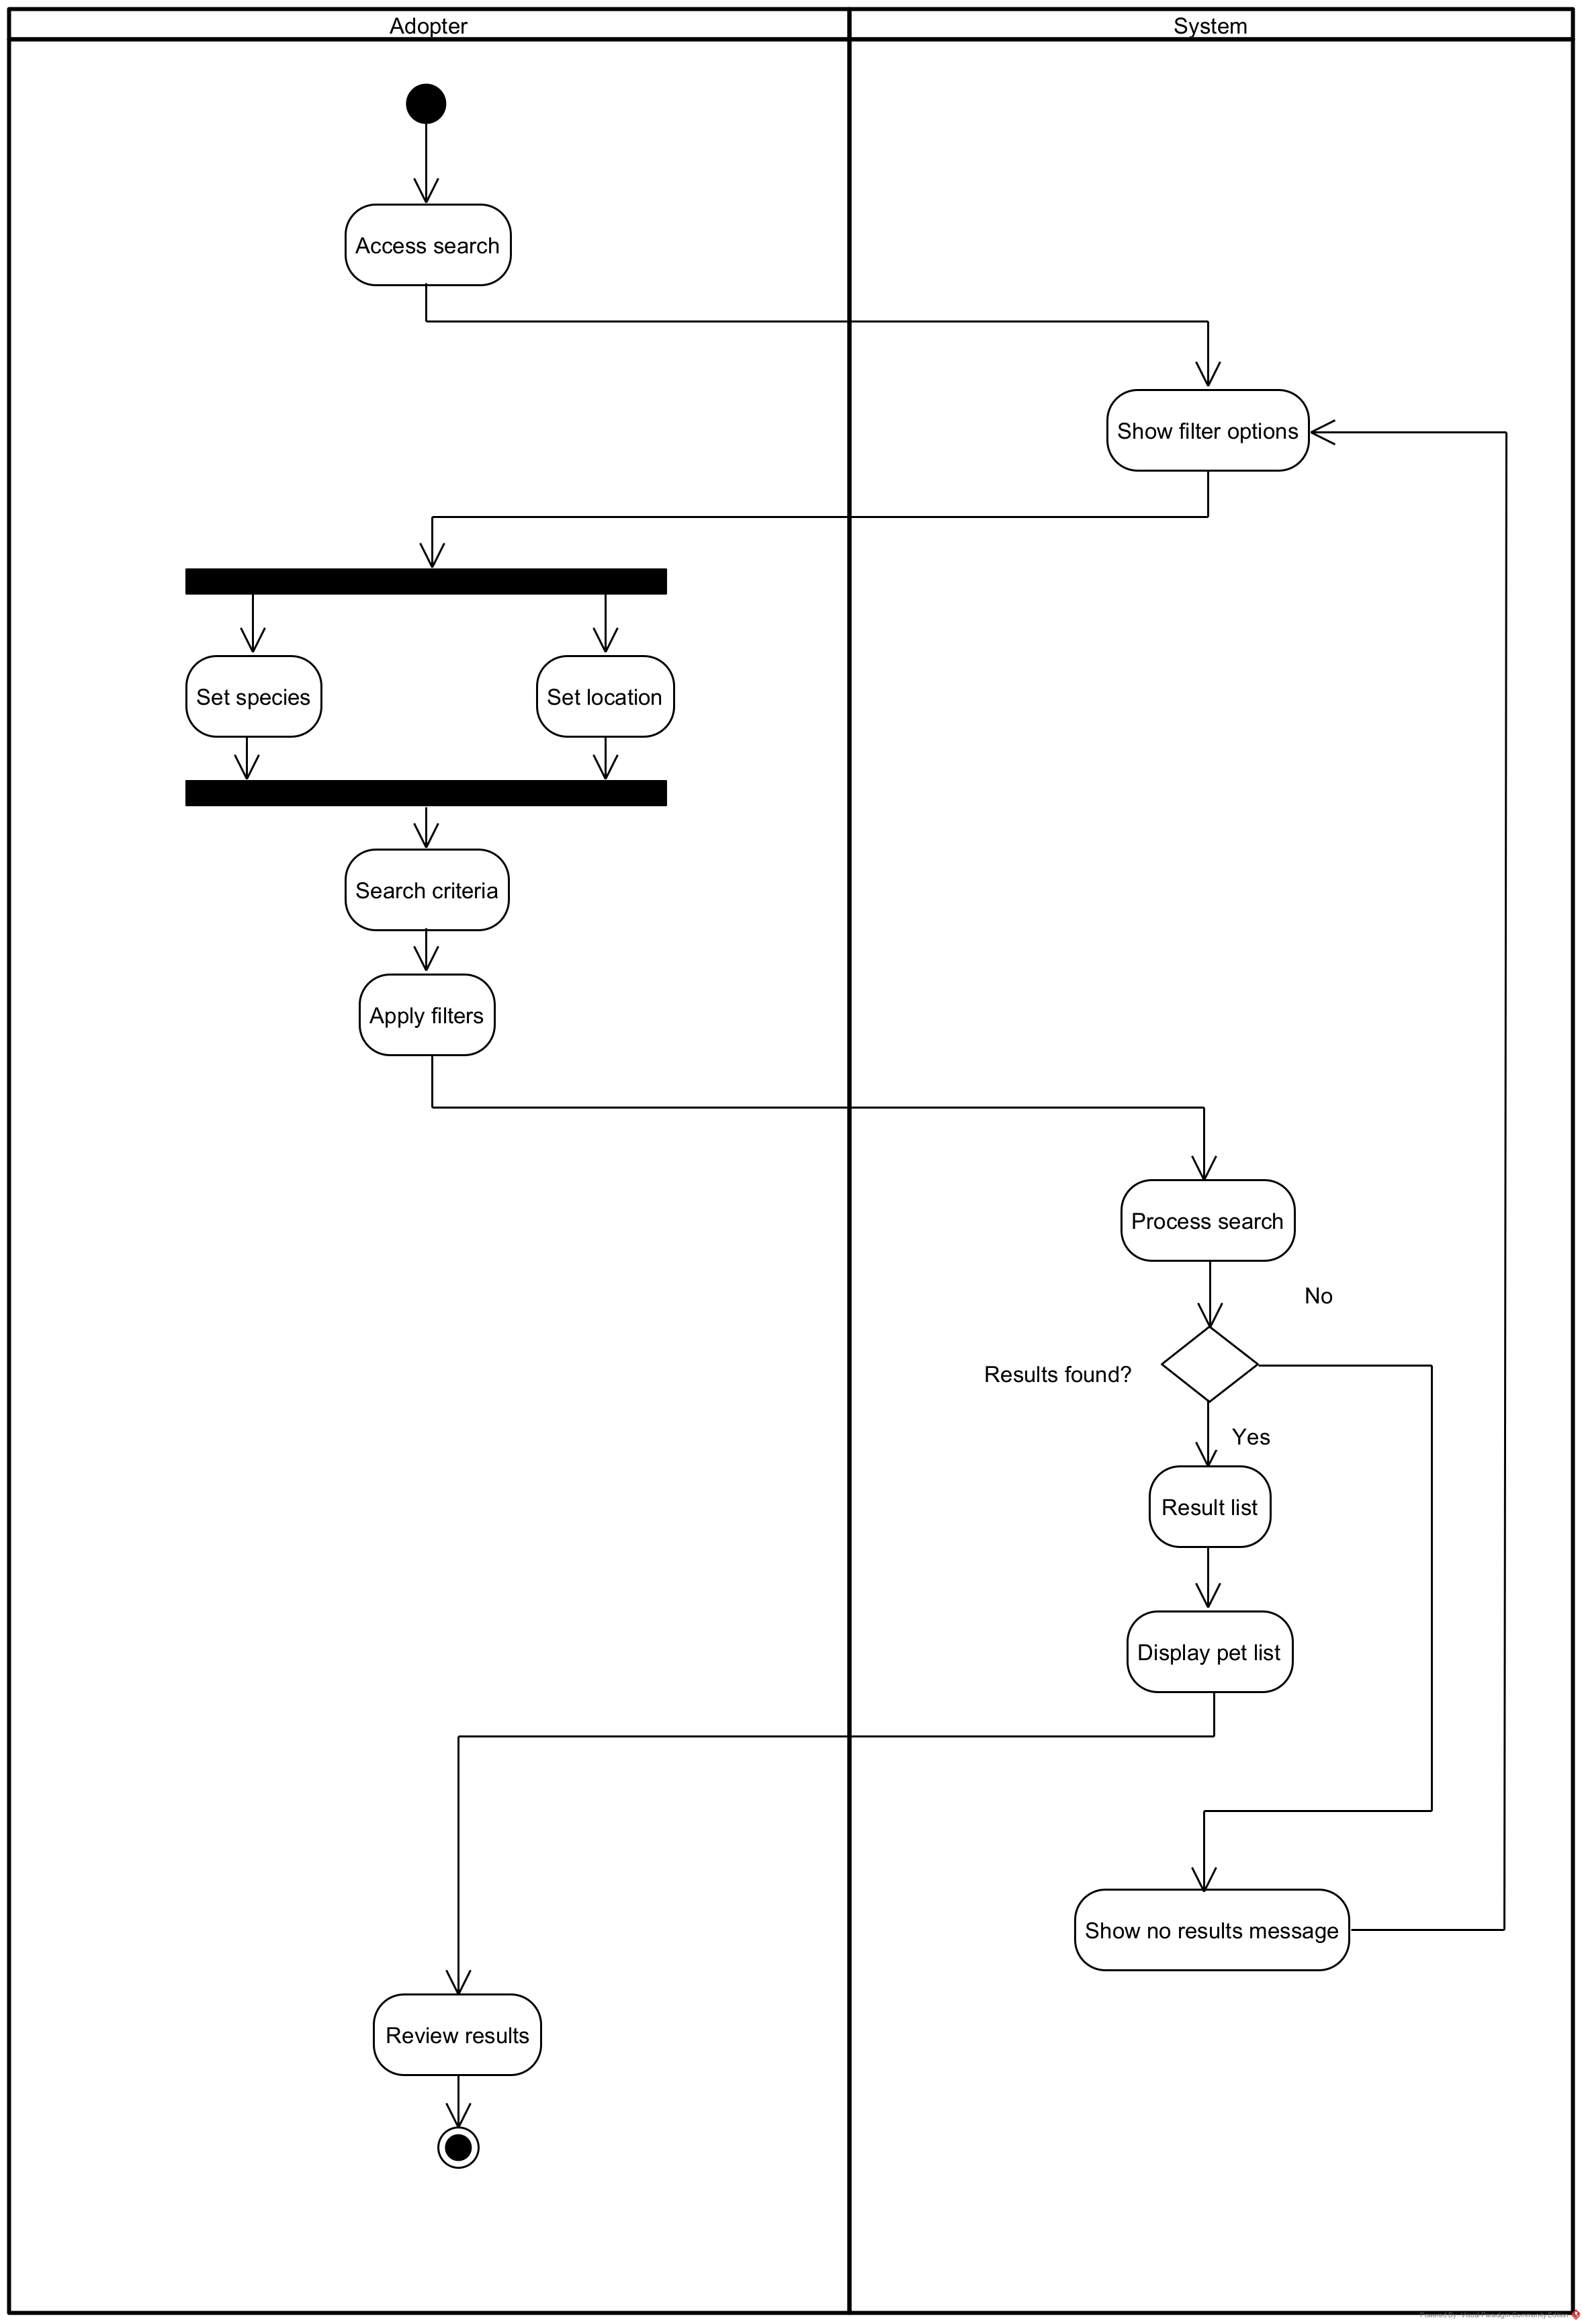
\includegraphics[width=0.95\textwidth]{DiagramaActividades_CU-11_MundiPets.png}
		\caption{Diagrama de actividades -- Buscar mascota disponible (CU-11).}
		\label{fig:act_cu11}
	\end{figure}
	
	Que ``Set species'' y ``Set location'' se definan como actividades
	paralelas (\textit{fork/join}) dentro de ``Apply filters'', tal como se
	ve en la Figura~\ref{fig:act_cu11}, revela que los criterios de búsqueda
	son independientes entre sí y combinables libremente, sin que uno
	dependa de haber definido antes el otro, permitiendo búsquedas parciales
	(solo especie, o solo ubicación).
	
	\subsubsection{Consultar recomendaciones de cuidado (CU-12)}
	
	\begin{figure}[H]
		\centering
		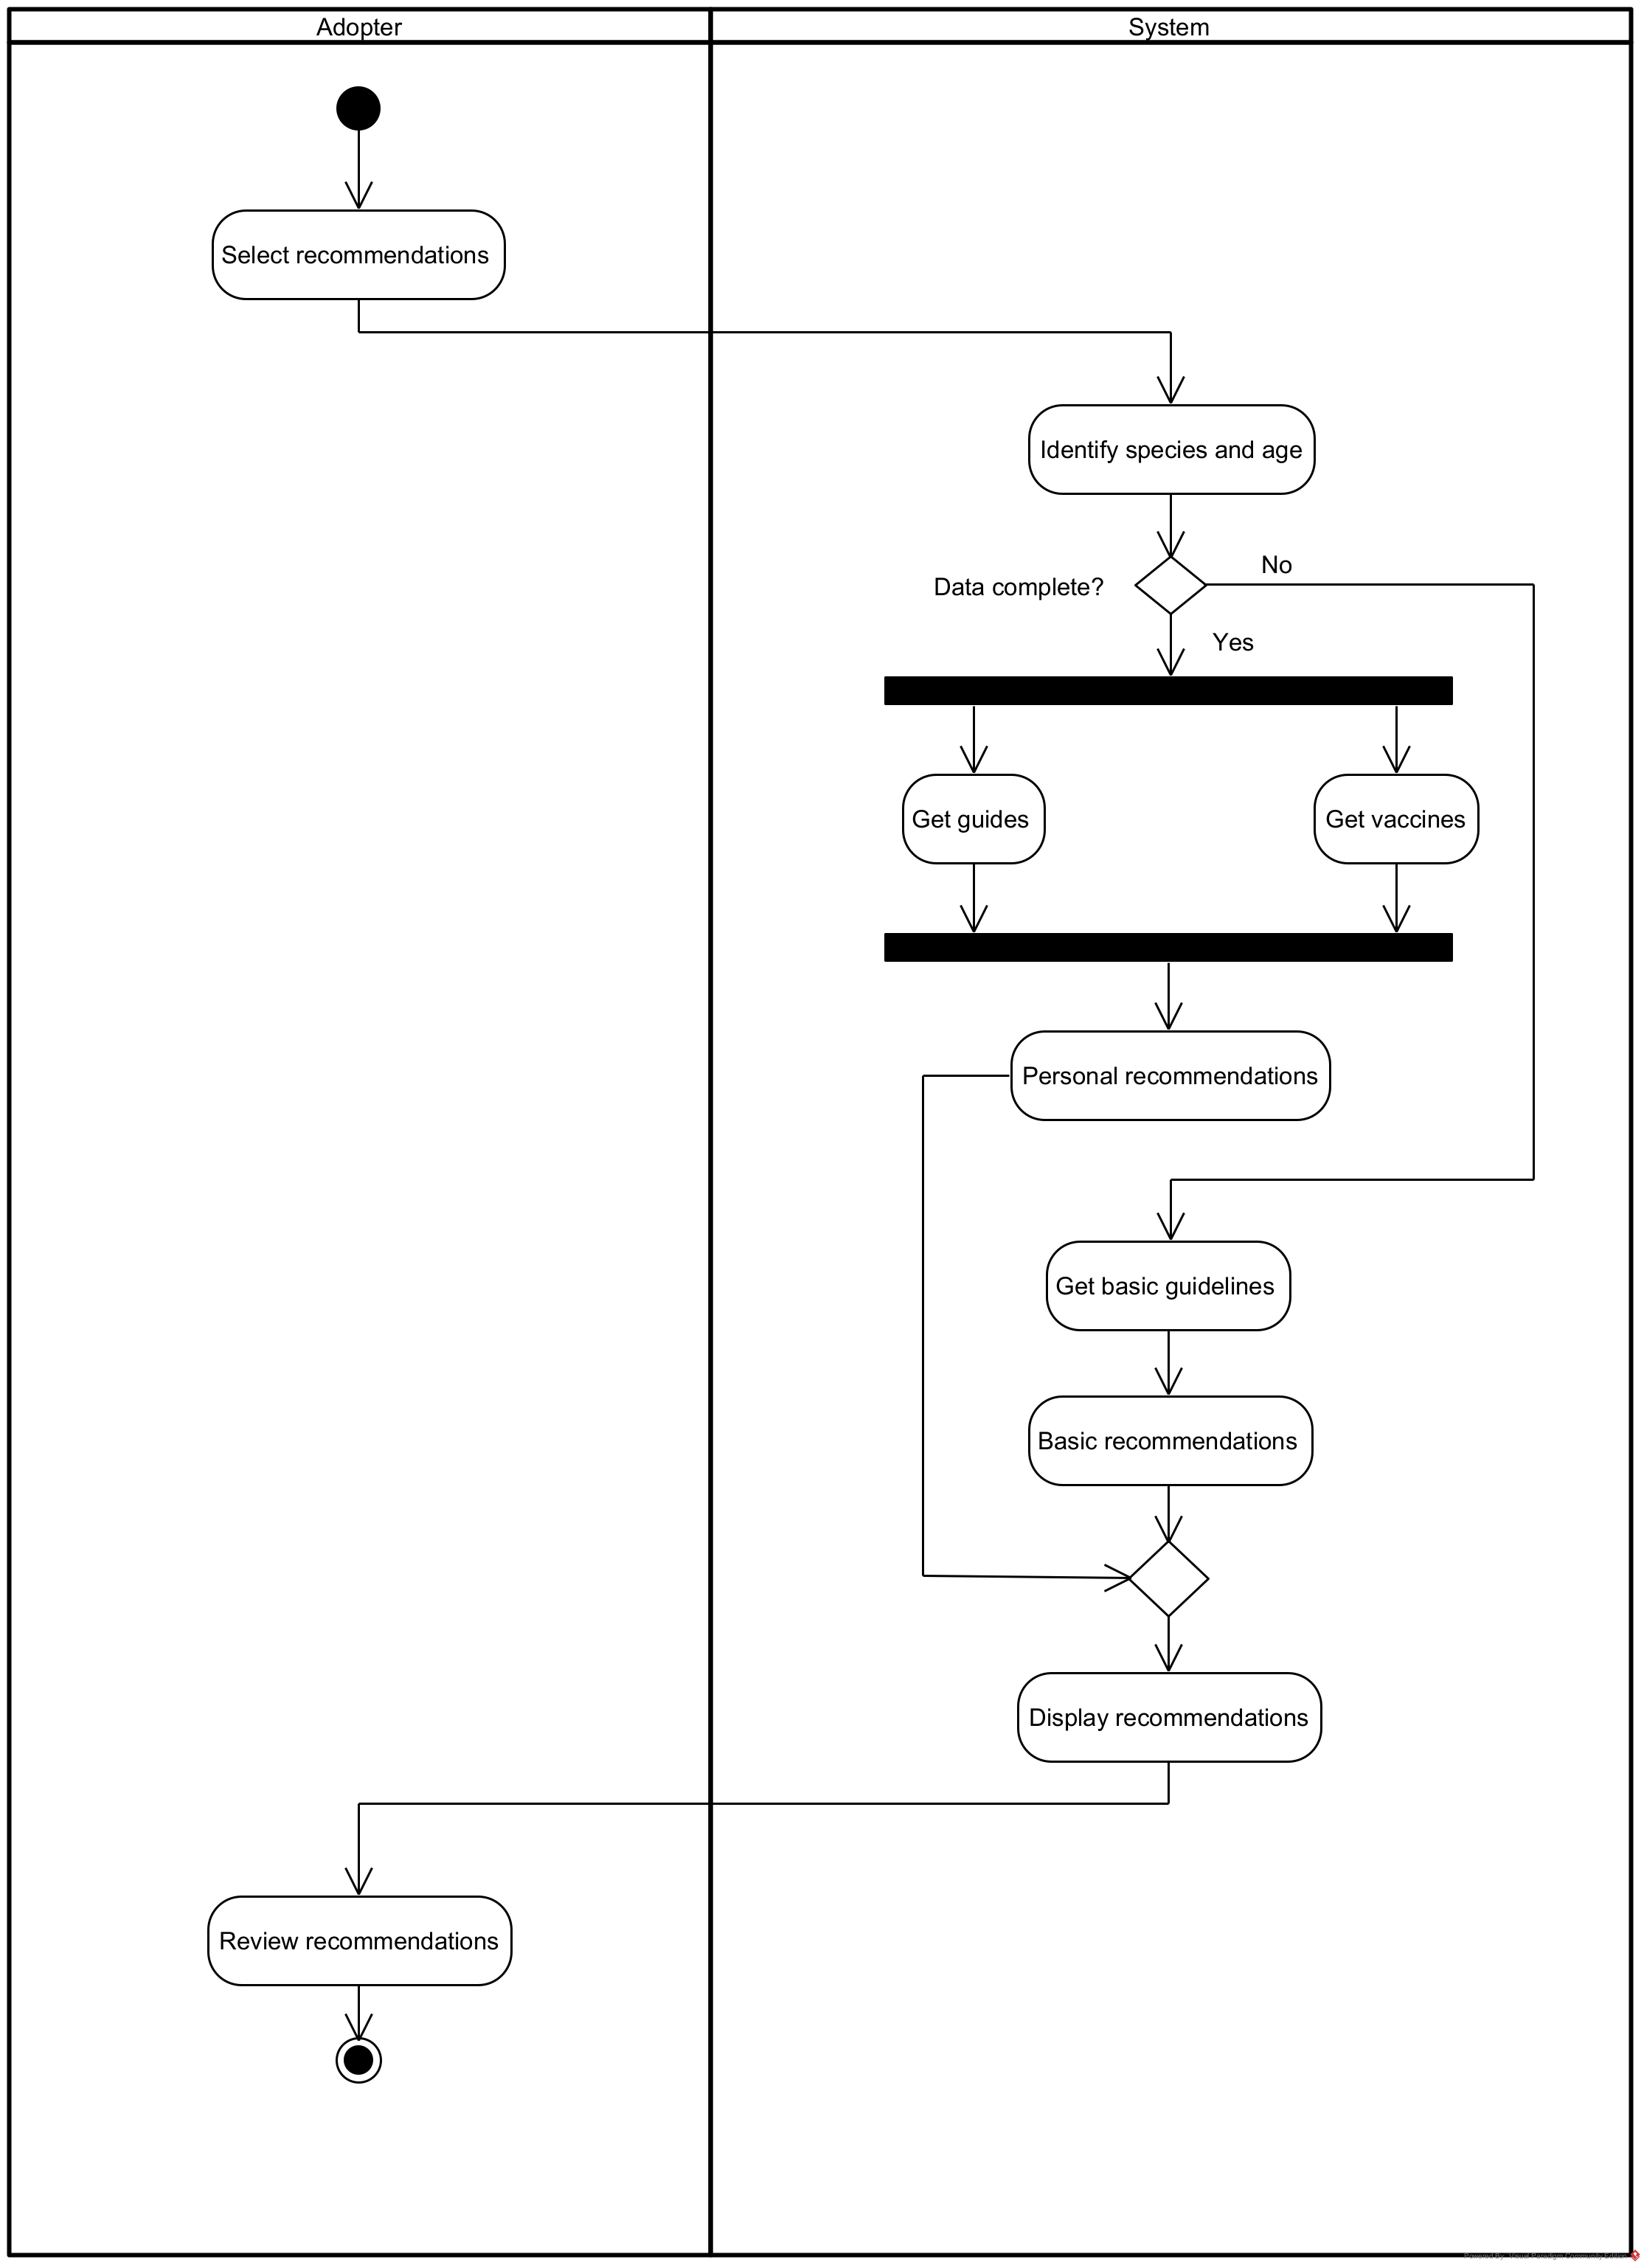
\includegraphics[width=0.85\textwidth]{DiagramaActividades_CU-12_MundiPets.png}
		\caption{Diagrama de actividades -- Consultar recomendaciones de cuidado (CU-12).}
		\label{fig:act_cu12}
	\end{figure}
	
	Que ``Data complete?'' con salida ``No'' desvíe directamente hacia ``Get
	basic guidelines'' (evitando por completo la rama paralela de ``Get
	guides''/``Get vaccines''), como se ve en la Figura~\ref{fig:act_cu12},
	revela que el sistema no intenta forzar al adoptante a completar el
	perfil antes de dar alguna recomendación: prefiere entregar un resultado
	genérico útil de inmediato en lugar de bloquear la funcionalidad por
	datos incompletos, igual que se observó en el diagrama de secuencia
	correspondiente (Figura~\ref{fig:sec_cu12}).
	
	\subsubsection{Evaluar compatibilidad de cruza (CU-13)}
	
	\begin{figure}[H]
		\centering
		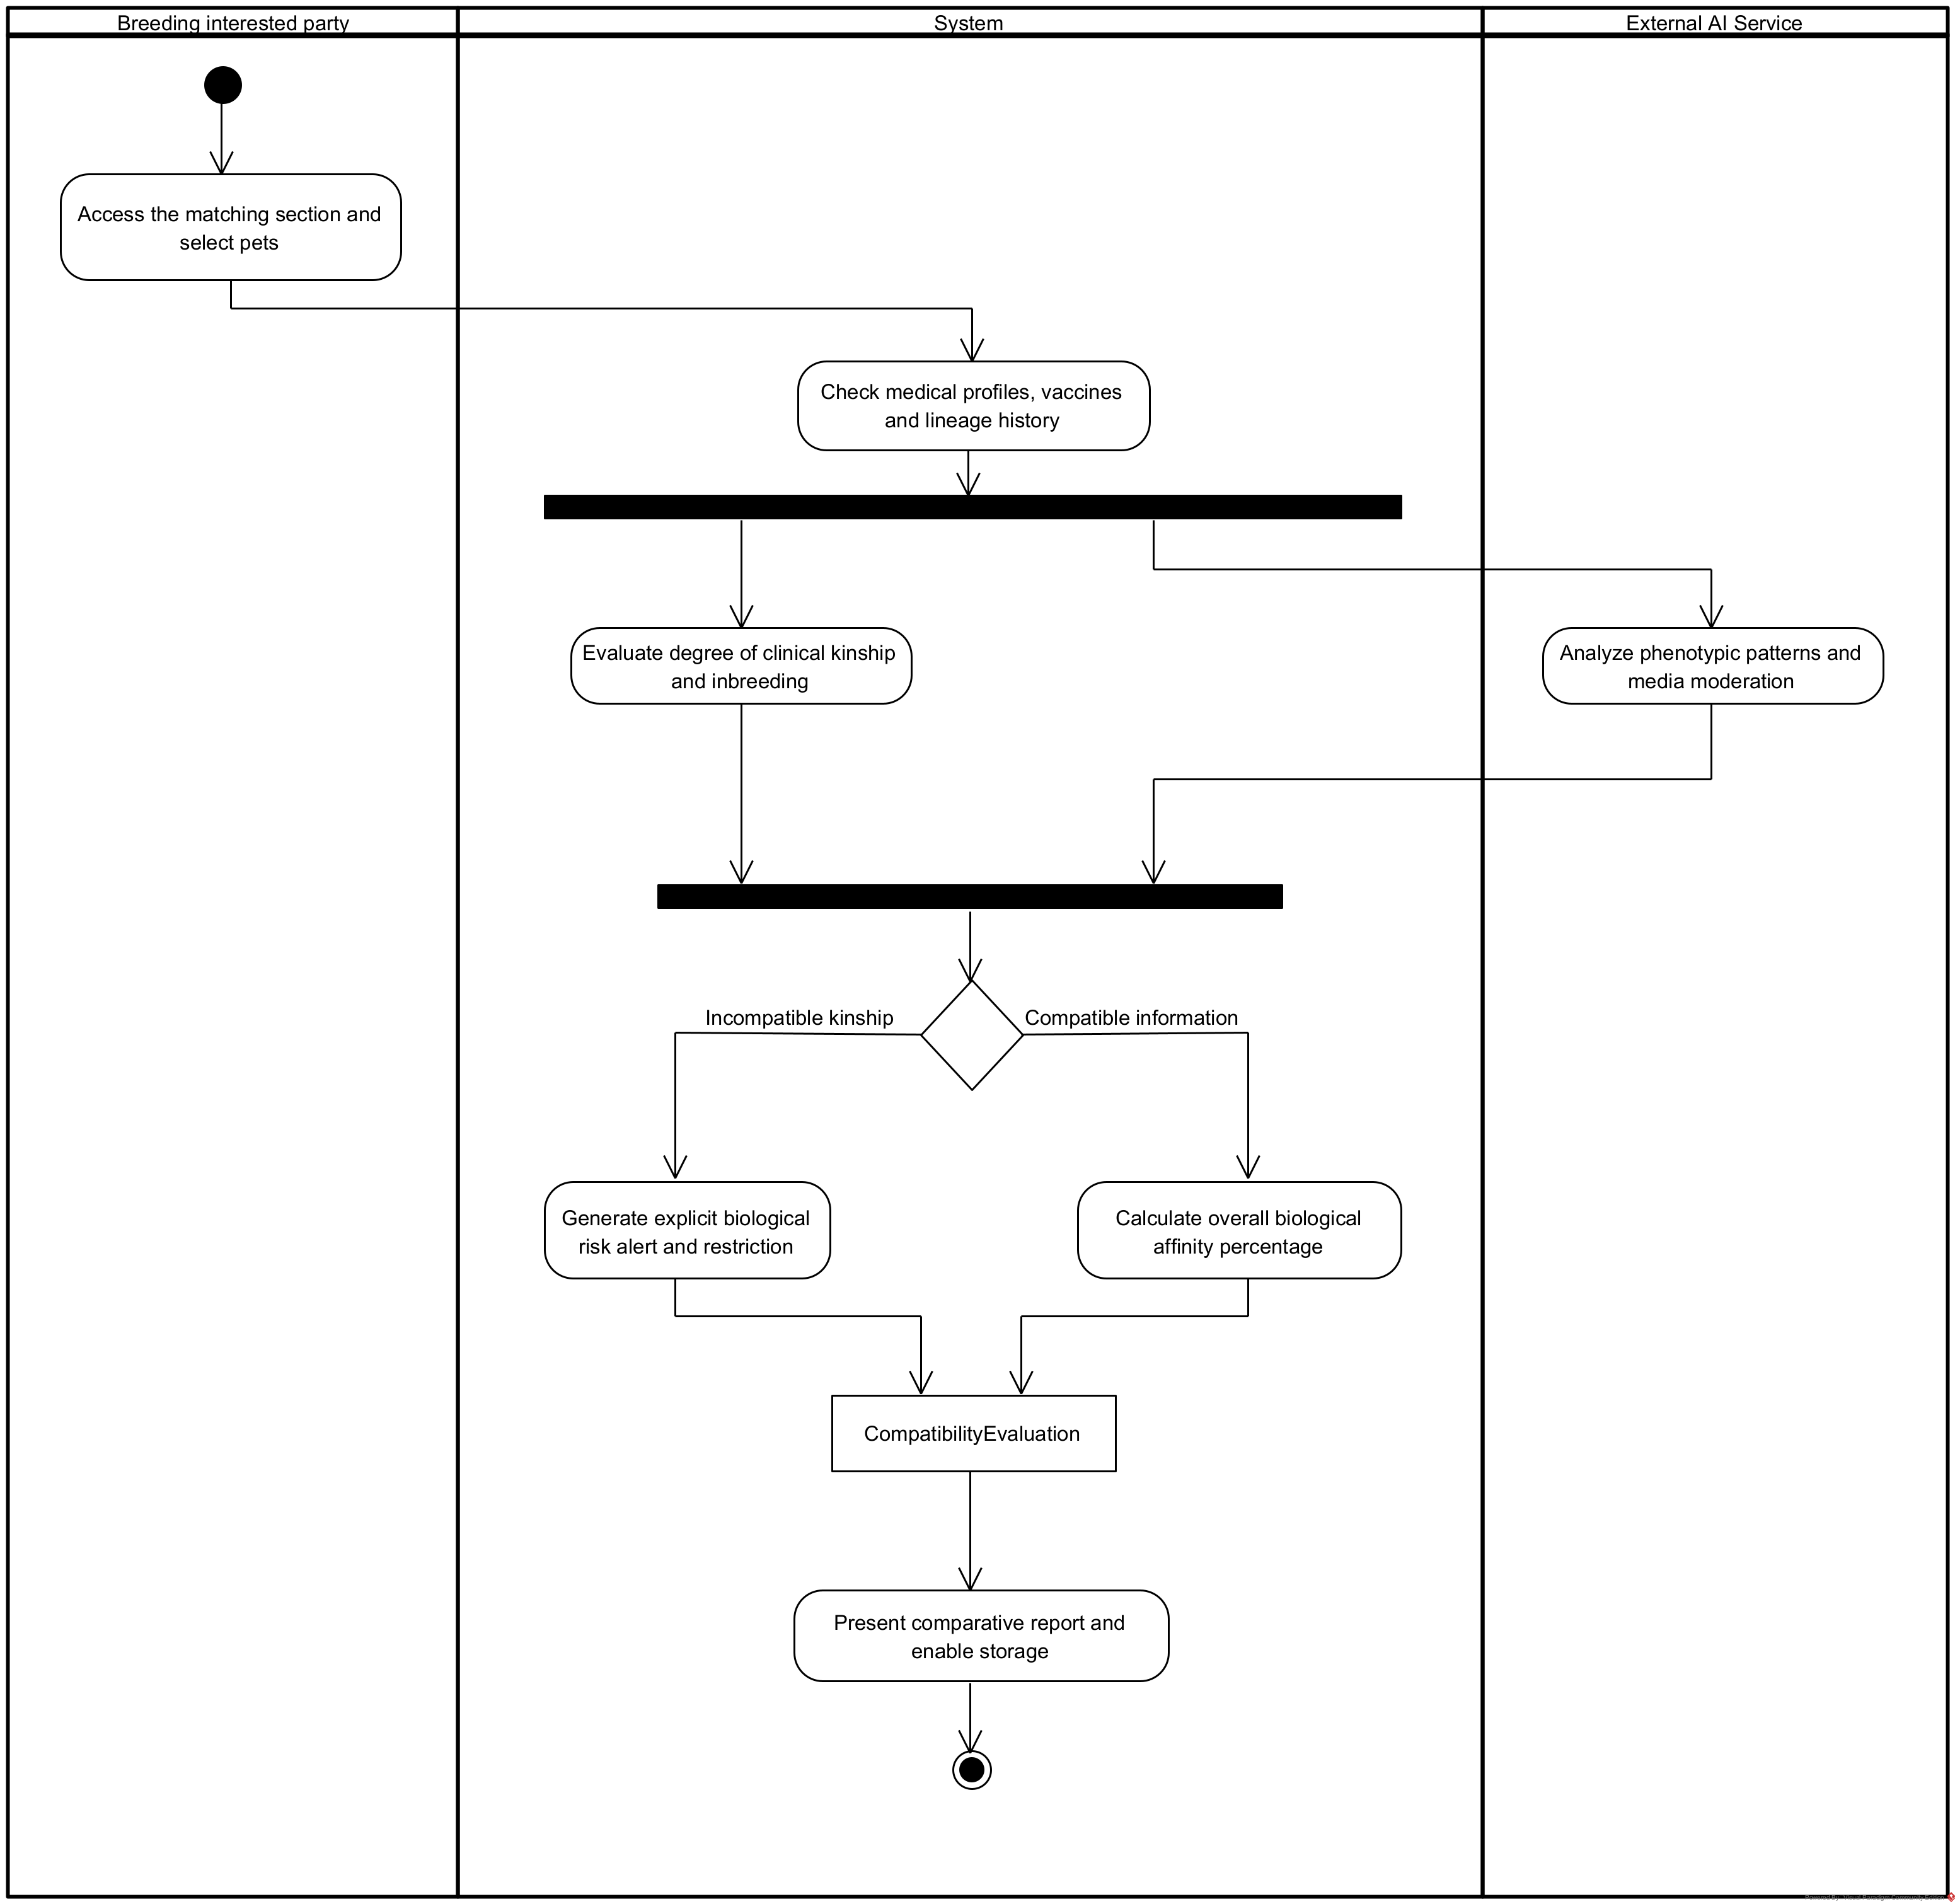
\includegraphics[width=0.95\textwidth]{DiagramaActividades_CU-13_MundiPets.png}
		\caption{Diagrama de actividades -- Evaluar compatibilidad de cruza (CU-13).}
		\label{fig:act_cu13}
	\end{figure}
	
	Que ``Evaluate degree of clinical kinship and inbreeding'' (carril
	\textit{System}) y ``Analyze phenotypic patterns and media moderation''
	(carril \textit{External AI Service}) se ejecuten en paralelo, pero que
	la decisión final (``Incompatible kinship'' vs.\ ``Compatible
	information'') dependa de fusionar ambos resultados antes de bifurcarse
	hacia ``Generate explicit biological risk alert'' o ``Calculate overall
	biological affinity percentage'', como se observa en la Figura~\ref{fig:act_cu13},
	revela visualmente el mismo principio observado en el diagrama de
	secuencia CU-13 (Figura~\ref{fig:sec_cu13}): el veredicto de riesgo
	determinista (parentesco) y el análisis probabilístico de la IA operan
	de forma independiente, pero la alerta de riesgo biológico tiene
	prioridad sobre el cálculo de afinidad cuando ambos resultados entran en
	conflicto.
	
	% ------------------------------------------------------------
	\subsection{Diagrama de Clases}
	
	\subsubsection{Usuarios y Roles}
	
	\begin{figure}[H]
		\centering
		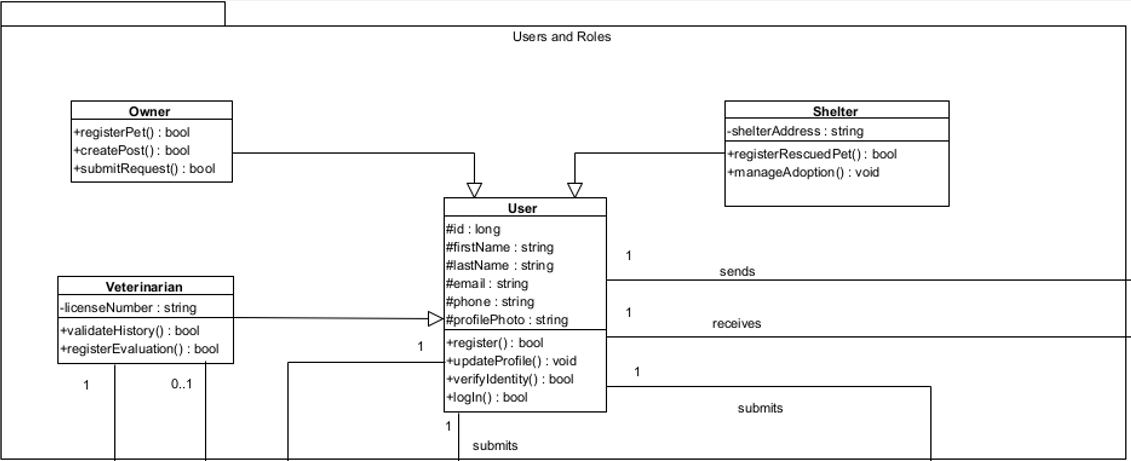
\includegraphics[width=0.95\textwidth]{DiagramaClasesUsersRoles.png}
		\caption{Diagrama de clases -- Usuarios y Roles.}
		\label{fig:clases_usuarios}
	\end{figure}
	
	Que ``Shelter'', ``Owner'' y ``Veterinarian'' hereden todos de una única
	clase base ``User'' (en lugar de modelarse como entidades independientes
	con su propia tabla de \textit{login}), como se observa en la
	Figura~\ref{fig:clases_usuarios}, revela que el sistema trata la
	identidad y autenticación como algo unificado y transversal, mientras
	que el comportamiento específico de cada actor
	(\textit{registerRescuedPet()}, \textit{validateHistory()}, etc.) se
	resuelve por especialización. La ausencia deliberada de una clase
	``Administrator'' (y de un mecanismo dinámico de roles tipo
	\textit{Role}/\textit{UserRole}) refleja que MundiPets opera como una
	plataforma entre pares sin un rol administrativo central: el tipo de
	usuario --- y por tanto sus permisos --- queda resuelto enteramente por
	la propia jerarquía de herencia, sin necesitar una capa de gestión de
	roles independiente que ningún requisito funcional respalda.
	
	\noindent\textit{Corrección aplicada (diagnóstico de cobertura,
	Sección~\ref{sec:trazabilidad}):} las clases \textit{Administrator},
	\textit{Role} y \textit{UserRole} se eliminaron de esta partición del
	diagrama de clases por constituir una cadena rota --- ningún RF ni CU
	las respaldaba---. El control de acceso por tipo de usuario queda
	completamente cubierto por la herencia \textit{Shelter}/\textit{Owner}/
	\textit{Veterinarian} $\rightarrow$ \textit{User}, ya utilizada de forma
	consistente en el campo ``Actor'' de los 27 requisitos funcionales del
	ERS.
	
	\subsubsection{Mascotas y Salud}

	\begin{figure}[H]
		\centering
		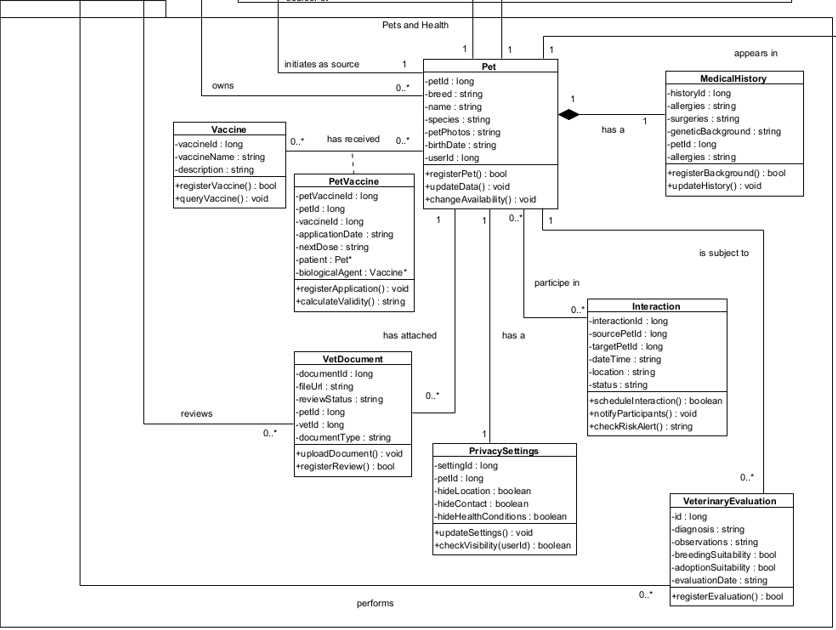
\includegraphics[width=0.85\textwidth]{DiagramaClasesPetsHealth.png}
		\caption{Diagrama de clases -- Mascotas y Salud.}
		\label{fig:clases_mascotas}
	\end{figure}

	Que ``MedicalHistory'' se relacione con ``Pet'' mediante una composición
	(rombo relleno, ``has a'' 1 a 1) y no una simple asociación, como se
	aprecia en la Figura~\ref{fig:clases_mascotas}, revela que el historial
	médico no tiene existencia independiente de la mascota: si se elimina el
	perfil de la mascota, su historial desaparece con él, a diferencia de
	``VeterinaryEvaluation'' o ``VetDocument'', que se asocian de forma más
	débil (0..*) y podrían sobrevivir como registros históricos aun si la
	mascota deja de estar activa. Por otro lado, que ``PetVaccine'' sea una
	clase de asociación entre ``Pet'' y ``Vaccine'' (con atributos propios
	como \textit{nextDose} y \textit{biologicalAgent}) en lugar de una
	relación directa, muestra que el sistema necesita rastrear cada
	aplicación individual de una vacuna (con su propia fecha y próxima
	dosis) y no solo si la mascota ``tiene'' cierta vacuna en abstracto. Que
	``Interaction'' reutilice el mismo patrón estructural que
	``BreedingRequest'' (dos referencias a ``Pet'', origen y destino, más un
	método \textit{checkRiskAlert()}) revela que el sistema reconoce que
	cualquier vínculo entre dos mascotas concretas, sea un encuentro de
	socialización o una solicitud de cruza, comparte el mismo riesgo
	biológico de fondo y debe validarse con la misma lógica, en lugar de
	duplicar esa regla de negocio en dos lugares distintos del modelo. Que
	``PrivacySettings'' se relacione con ``Pet'' mediante composición 1 a 1
	(``has a''), igual que ``MedicalHistory'', muestra que la configuración
	de privacidad no es un ajuste global de la cuenta del usuario, sino un
	dato que pertenece y viaja con cada mascota individual: dos mascotas del
	mismo propietario pueden tener reglas de visibilidad distintas entre sí.

	\subsubsection{Comunicación y Publicaciones}

	\begin{figure}[H]
		\centering
		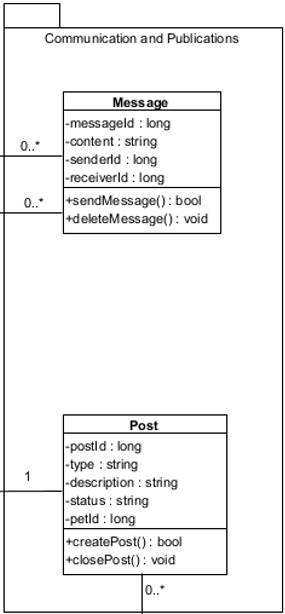
\includegraphics[width=0.4\textwidth]{DiagramaClasesComunicatiosPublicatios.png}
		\caption{Diagrama de clases -- Comunicación y Publicaciones.}
		\label{fig:clases_comunicacion}
	\end{figure}

	Que ``Message'' siga sin ninguna relación directa con ``Post'', ni
	siquiera ahora que existe ``Interaction'' para modelar encuentros
	presenciales (partición Mascotas y Salud), como se observa en la
	Figura~\ref{fig:clases_comunicacion}, refuerza la misma lectura de
	diseño ya identificada: la mensajería es un canal transversal entre
	usuarios, desacoplado tanto del contexto de una publicación como del
	registro formal de un encuentro coordinado. Esto evita que ``Message''
	termine sobrecargado con responsabilidades que no le corresponden
	(agendar, registrar ubicación, marcar estado de un encuentro), las
	cuales fueron correctamente delegadas a una clase propia
	(``Interaction'') en lugar de resolverse con campos adicionales dentro
	del propio mensaje.

	\subsubsection{Solicitudes y Evaluaciones}

	\begin{figure}[H]
		\centering
		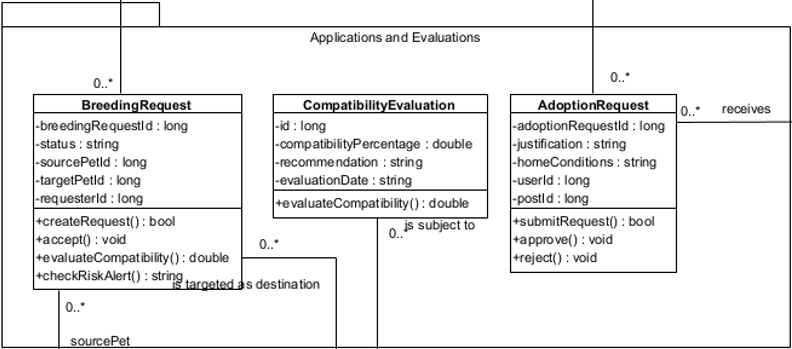
\includegraphics[width=0.95\textwidth]{DiagramaClasesAplicationsEvaluations.png}
		\caption{Diagrama de clases -- Solicitudes y Evaluaciones.}
		\label{fig:clases_solicitudes}
	\end{figure}

	Que \textit{checkRiskAlert()} se agregue como método propio de
	``BreedingRequest'' (y no como una clase de evaluación independiente, a
	diferencia de ``CompatibilityEvaluation''), como se ve en la
	Figura~\ref{fig:clases_solicitudes}, revela que la alerta de riesgo
	sanitario o físico se trató deliberadamente como una validación
	transitoria calculada al momento de crear la solicitud, no como un
	resultado que deba persistirse y auditarse después: mientras
	``CompatibilityEvaluation'' sí se guarda como registro propio (porque su
	recomendación debe poder consultarse más adelante), la alerta de riesgo
	solo necesita bloquear o advertir en el instante de la confirmación, y
	desaparece una vez tomada la decisión.

	\subsubsection{Vista Refinada General}
	
	\begin{figure}[H]
		\centering
		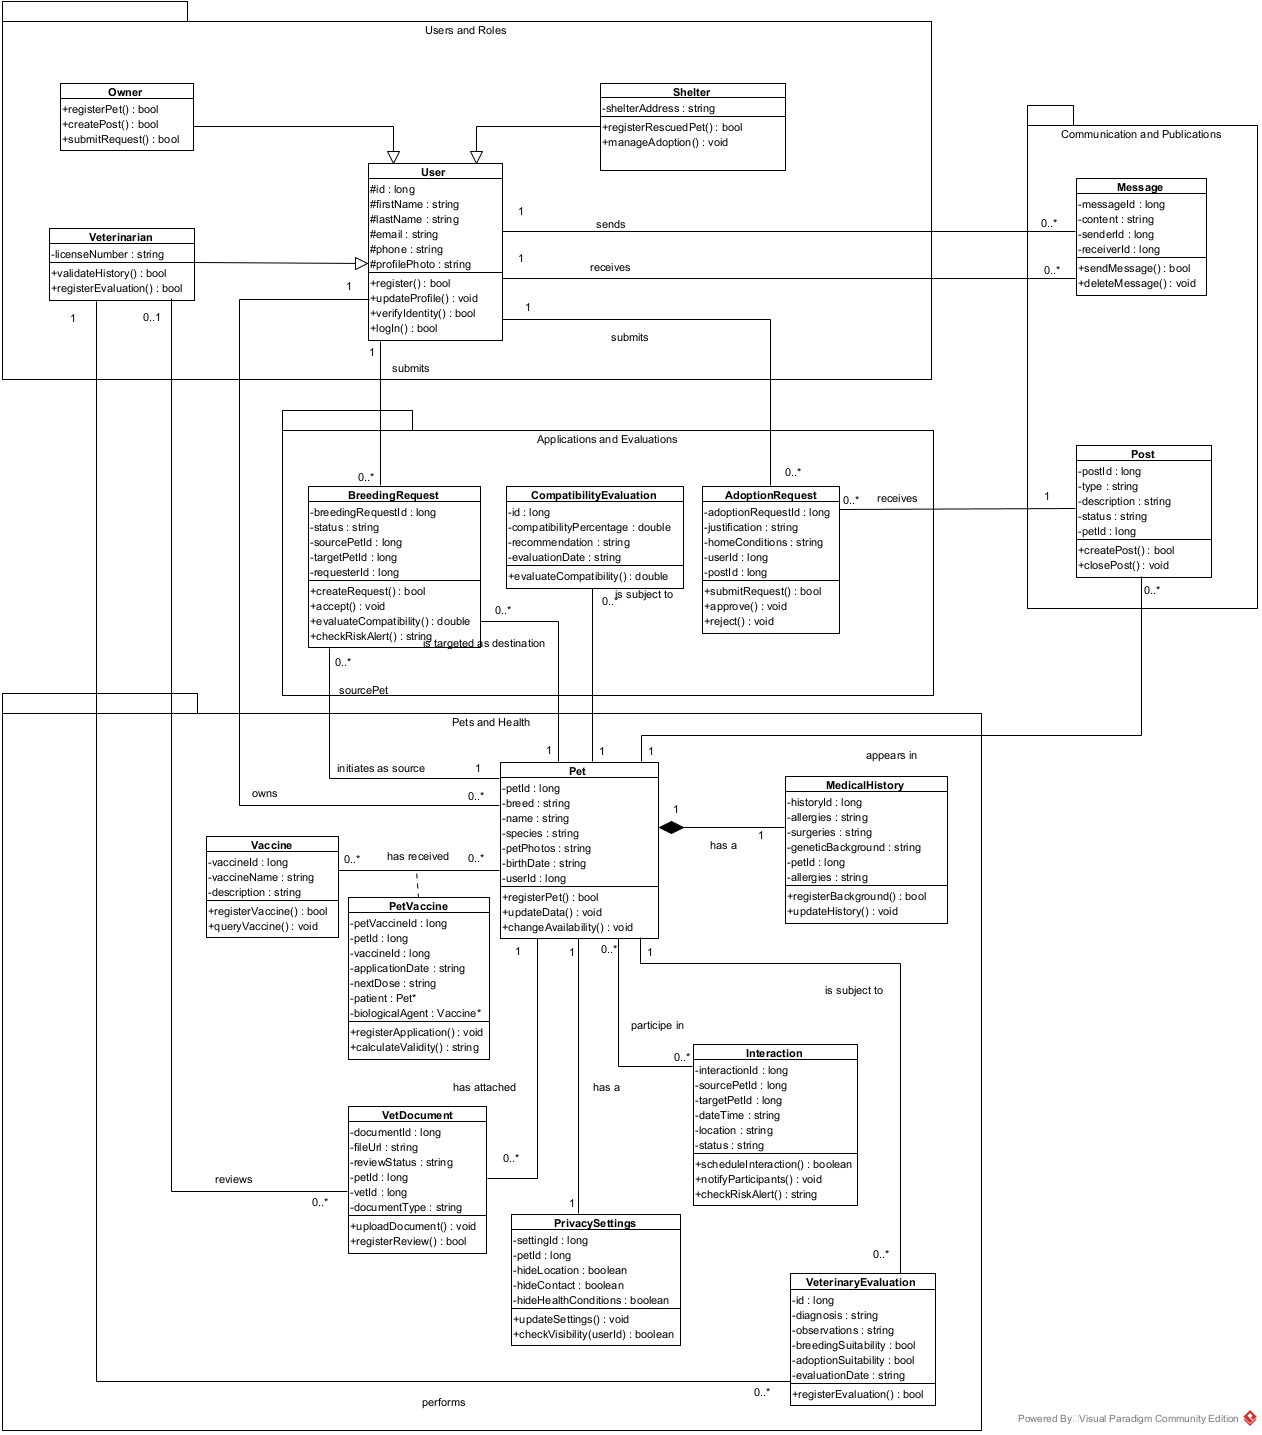
\includegraphics[width=0.95\textwidth]{DiagramaClasesRefinado_MundiPets.png}
		\caption{Diagrama de clases -- Vista refinada general (integración de las cuatro particiones).}
		\label{fig:clases_refinado}
	\end{figure}
	
	Que ``Pet'' sea la clase con más conexiones entrantes de todo el
	diagrama (origen de ``AdoptionRequest'', ``BreedingRequest'' vía
	\textit{sourcePet}/``is targeted as destination'', ``MedicalHistory'',
	``PetVaccine'', ``VetDocument'',
	``VeterinaryEvaluation'' y ``Post''), como se observa en la
	Figura~\ref{fig:clases_refinado}, confirma visualmente lo que ya el
	diagrama de Contexto (Figura~\ref{fig:contexto}) y la matriz de
	trazabilidad (Sección~\ref{sec:trazabilidad}) venían señalando: la
	mascota es el agregado central del dominio de MundiPets, y prácticamente
	ningún proceso (adopción, cruza, salud, comunicación) tiene sentido sin
	anclarse primero a un ``Pet'' concreto. Esto también explica por qué la
	Sección~\ref{sec:metricas} (trazabilidad) probablemente encuentre más
	filas asociadas a RF relacionados con ``Pet'' que con cualquier otra
	entidad, y por qué un defecto en el modelo de ``Pet'' tendría el radio
	de impacto más amplio de todo el sistema (relevante para M5,
	modificabilidad).
	
	\noindent\textit{Corrección aplicada (diagnóstico de cobertura,
	Sección~\ref{sec:trazabilidad}):} la clase \textit{VeterinaryAppointment}
	(agendar/cancelar citas) se elimina de esta partición por constituir una
	cadena rota que además contradice dos exclusiones de alcance declaradas
	explícitamente en el ERS: MundiPets no reemplaza la consulta veterinaria
	presencial ni ofrece una agenda médica completa de clínicas. RF-10
	(recordatorios de controles preventivos) cubre únicamente el aviso
	pasivo de vacunas y controles próximos, no la reserva activa de un turno
	dentro del sistema, por lo que ambas funciones no deben confundirse.
	
	\newpage
	
	% ============================================================
	%  SECCION 5 -- VALIDACION
	% ============================================================
	

ewpage

% ============================================================
%  SECCION 6 -- GESTION Y TRAZABILIDAD
% ============================================================
\section{Gestión y Trazabilidad}
\label{sec:trazabilidad}

% -- 6.1 --------------------------------------------------------
\subsection{Línea base y control de cambios}

Durante la Práctica Experimental 4 (PE4), el docente conformó grupos de
inspección ajenos a los equipos del PFC. Como resultado, el ERS de
MundiPets fue inspeccionado de manera independiente por cuatro
subgrupos, cada uno integrado por un miembro del equipo del PFC junto
con compañeros externos: Fuertes--Contreras--Viteri, Cedeño
Ávila--Córdova--Mendoza, Morales--Sánchez--Cedeño y Gutiérrez--Nieves.
Cada subgrupo tramitó tres RFC ante un Change Control Board (CCB)
simulado, sobre su propia copia de trabajo del ERS. En total se
generaron 12 formularios RFC, de los cuales tres correspondían al mismo
hallazgo detectado de forma independiente por tres subgrupos distintos,
quedando 10 solicitudes de cambio únicas. La Tabla~\ref{tab:rfc_registro}
consolida estas 10 RFC, su decisión del CCB y su justificación.

\begin{table}[H]
	\centering
	\caption{Registro de RFC tramitados en la PE4 sobre el ERS de MundiPets.}
	\label{tab:rfc_registro}
	\small
	\begin{tabularx}{\textwidth}{|c|X|X|X|c|}
		\hline
		\textbf{RFC} & \textbf{Requisito afectado} & \textbf{Decisión} & \textbf{Justificación} & \textbf{Fecha} \\
		\hline
		RFC-A & RF-25, RNF-16 & Aprobado / Aprobado con condiciones (3 subgrupos) & RNF-16 (base legal LOPDP) exige ocultar ubicación/contacto por defecto; RF-25 los exponía & 08--09/08/2026 \\
		\hline
		RFC-B & RD-06, RL-04 & Aprobado & El propio RD-06 reconoce que ningún RF implementa el derecho de eliminación (Art. 15 LOPDP) & 09/08/2026 \\
		\hline
		RFC-C & RF-10, RD-08 & Aprobado & RD-08 exige canal de respaldo ante caída de WhatsApp, pero RF-10 no lo formaliza & 09/08/2026 \\
		\hline
		RFC-D & RNF-09, RD-08 & Aprobado con condiciones & Comprometer un proveedor de pago (WhatsApp) sin presupuesto aprobado es inviable & 09/08/2026 \\
		\hline
		RFC-E & RNF-02 & Aprobado & El MVP local no permite verificar disponibilidad mensual del 99\,\% & 09/08/2026 \\
		\hline
		RFC-F & RF-07, RNF-15 & Aprobado con condiciones & El ERS reconoce el conflicto ``comunicación inadecuada'' sin RF que lo resuelva & 08/08/2026 \\
		\hline
		RFC-G & RNF-03 & Aprobado con condiciones & El umbral de 2s no era verificable con la infraestructura disponible & 08/08/2026 \\
		\hline
		RFC-H & RF-07, RNF-15 & Aprobado con condiciones & RNF-15 exige explicabilidad de una moderación que ningún RF especifica & 09/08/2026 \\
		\hline
		RFC-I & RF-06, RNF-06, RNF-13 & Aprobado & RNF-06/RNF-13 califican una salida que RF-06 no declaraba producir & 09/08/2026 \\
		\hline
		RFC-J & RF-01, RF-27, RL-01 & Aprobado & El consentimiento debe ser revocable en cualquier momento (Art. 7 y 8 LOPDP) & 09/08/2026 \\
		\hline
	\end{tabularx}
\end{table}

Ningún CCB de los cuatro subgrupos de la PE4 rechazó una RFC: las 10
solicitudes únicas fueron aprobadas o aprobadas con condiciones sobre la
copia de trabajo de cada subgrupo. Sin embargo, ninguna de esas
aprobaciones se tradujo automáticamente en un cambio sobre el
repositorio único del PFC, ya que cada subgrupo trabajó de forma
independiente sobre su propia copia del documento. Por ello, como parte
del cierre de la PE5, el equipo del PFC convocó un nuevo CCB para
decidir formalmente sobre las 10 RFC frente a la línea base real de
MundiPets. De esas 10: una ya estaba resuelta en el ERS vigente (RFC-A);
cinco se aplicaron directamente (RFC-C, RFC-E, RFC-F, RFC-I, y la
corrección de alcance derivada de RFC-G); una se resolvió reacotando un
requisito no funcional ya existente, sin crear un requisito funcional
nuevo (RFC-H); y tres fueron rechazadas con justificación registrada,
por preferirse una alternativa (RFC-D) o por no contar con evidencia de
entrevista que sustentara un requisito funcional nuevo y verificable
(RFC-B, RFC-J). La Tabla~\ref{tab:rfc_estado} documenta la decisión final
de cada una; ninguna RFC permanece sin resolver al cierre de la PE5.

\begin{table}[H]
	\centering
	\caption{Estado de incorporación en la línea base vigente (ERS v4.0).}
	\label{tab:rfc_estado}
	\small
	\begin{tabularx}{\textwidth}{|c|X|X|}
		\hline
		\textbf{RFC} & \textbf{Origen (subgrupo PE4)} & \textbf{Decisión final del CCB (cierre PE5)} \\
		\hline
		RFC-A & Fuertes, Morales, Gutiérrez/Nieves & Resuelto: ya estaba correcto en el ERS \\
		\hline
		RFC-B & Mendoza & Rechazado, con justificación: crear el RF sin evidencia de entrevista lo volvería no verificable. RD-06 se mantiene como restricción reconocida \\
		\hline
		RFC-C & Mendoza & Aplicado: RF-10 corregido \\
		\hline
		RFC-D & Morales & Rechazado: se prefirió RFC-C como solución al mismo problema \\
		\hline
		RFC-E & Mendoza & Aplicado: RNF-02 corregido \\
		\hline
		RFC-F & Fuertes & Aplicado: RF-07 corregido \\
		\hline
		RFC-G & Fuertes & Rechazada la propuesta original (relajar el umbral); resuelto por vía alternativa: RNF-03 acotado a producción, igual que RNF-02 \\
		\hline
		RFC-H & Morales & Resuelto: RNF-15 reacotado a RF-07, sin crear RF nuevo \\
		\hline
		RFC-I & Gutiérrez/Nieves & Aplicado: RF-06 corregido \\
		\hline
		RFC-J & Gutiérrez/Nieves & Rechazado, con justificación: requeriría un RF con efectos en cascada no verificable sin evidencia. RL-01 queda con brecha reconocida, no con RFC abierta \\
		\hline
	\end{tabularx}
\end{table}

A la fecha de cierre de esta PE5, el equipo aún no ha establecido una
línea base formal sobre el repositorio del PFC
(\url{https://github.com/andymendozap03/MundiPets-PFC-IngReq}). Para
declarar la línea base final, corresponde ejecutar:

\begin{verbatim}
git tag -a baseline-vX.X -m "Linea base final ERS MundiPets - PE5"
git push origin baseline-vX.X
\end{verbatim}

\noindent y completar en esta sección el número de versión, la fecha y
el \textit{hash} del commit sobre el que quedó anclado el tag, de modo
que la línea base sea auditable conforme exige el criterio C2 de la
rúbrica.

% -- 6.2 --------------------------------------------------------
\subsection{Matriz de trazabilidad final}

La Tabla~\ref{tab:matriz_final} consolida la trazabilidad end-to-end de
los 43 elementos vigentes del ERS (27 RF y 16 RNF), siguiendo la cadena
mínima exigida para el PFC: Fuente/Stakeholder, RF/RNF, CU, Clase UML,
Proceso DFD, Estado, Criterio BDD, Caso de Prueba conceptual e Historia
del backlog, más una columna de trazabilidad horizontal (relación entre
requisitos del mismo nivel) solicitada adicionalmente por el docente. El
Proceso DFD corresponde a los seis procesos del Diagrama de Flujo de
Datos Nivel 1 (P1 a P6, Figura~\ref{fig:dfd_nivel1}), que descompone el
proceso único ``0. MundiPets'' del Diagrama de Contexto
(Figura~\ref{fig:contexto}). La columna Fuente identifica al
participante de origen mediante su código de evidencia (PROP-XX para
propietarios, VET-XX para veterinarias, OBS-01 para la observación de
campo y Encuesta para el cuestionario digital agregado), conforme lo
solicitó el docente en lugar del identificador EV-XX. Un enlace se marca
únicamente cuando existe evidencia textual verificable en el ERS o en
los modelos de la Sección 4; los eslabones sin relación real se marcan
con ``---''.

\begin{landscape}
\begin{table}[H]
	\centering
	\caption{Matriz de Trazabilidad Final del ERS de MundiPets.}
	\label{tab:matriz_final}
	\tiny
	\begin{tabularx}{\linewidth}{|l|X|X|c|X|c|c|c|c|c|X|}
		\hline
		\textbf{RF/RNF} & \textbf{Fuente} & \textbf{Horizontal} & \textbf{CU} & \textbf{Clase UML} & \textbf{DFD} & \textbf{Estado} & \textbf{BDD} & \textbf{CP} & \textbf{Hist.} & \textbf{Estado de la traza} \\
		\hline
		RF-01 & PROP-02, VET-01, VET-03, OBS-01 & RF-12 & CU-01 & Pet & P1 & Perfil Mascota & CA-01 & CP-01 & HU-01 & Completa \\ \hline
		RF-02 & PROP-01, VET-02 & RF-14 & CU-02 & MedicalHistory, Pet & P2 & --- & CA-02 & CP-02 & HU-02 & Completa \\ \hline
		RF-03 & VET-02, PROP-03, OBS-01 & RF-11 & CU-10 & Pet, MedicalHistory & P2 & --- & CA-03 & CP-03 & HU-03 & Completa \\ \hline
		RF-04 & Encuesta, OBS-01 & --- & CU-11 & Post, Pet & P3 & --- & --- & CP-04 & --- & Completa (Should) \\ \hline
		RF-05 & PROP-01, PROP-02, VET-01, OBS-01 & RF-13 & CU-04 & Post & P3 & Perfil Mascota & CA-04 & CP-05 & HU-04 & Completa \\ \hline
		RF-06 & VET-02, VET-03, PROP-03, OBS-01 & RNF-13, RF-02, RF-16 & CU-13 & CompatibilityEvaluation, Pet & P4 & --- & CA-05 & CP-06 & HU-05 & Completa \\ \hline
		RF-07 & PROP-02, Encuesta, OBS-01 & RNF-15 & CU-08 & Message & P5 & --- & --- & CP-07 & --- & Completa (Could) \\ \hline
		RF-08 & PROP-01, VET-01, VET-03 & RF-27 & CU-05 & BreedingRequest & P3 & Solicitudes & CA-06 & CP-08 & HU-06 & Completa \\ \hline
		RF-09 & VET-01, VET-03, Encuesta & RF-26, RF-19 & CU-09 & VeterinaryEvaluation, MedicalHistory & P2 & Verif. Documentos & CA-07 & CP-09 & HU-07 & Completa \\ \hline
		RF-10 & PROP-02, VET-02, PROP-03 & RD-08 & CU-12 & Pet, PetVaccine & P5 & --- & --- & CP-10 & --- & Completa (Should) \\ \hline
		RF-11 & PROP-02, VET-03, PROP-03, Encuesta, OBS-01 & RF-03, RNF-01, RNF-16 & CU-06 & PrivacySettings & P1 & --- & CA-08 & CP-11 & HU-08 & Completa \\ \hline
		RF-12 & PROP-01, VET-01, Encuesta, OBS-01 & RF-01 & (Onboarding) & User & P1 & --- & CA-09 & CP-12 & HU-09 & Completa \\ \hline
		RF-13 & PROP-01, PROP-02, Encuesta, OBS-01 & RF-05 & CU-04 & Post & P3 & --- & CA-10 & CP-13 & HU-10 & Completa \\ \hline
		RF-14 & VET-01, VET-03, Encuesta & RF-02, RF-24 & CU-03 & PetVaccine, VetDocument & P2 & Verif. Documentos & CA-11 & CP-14 & HU-11 & Completa \\ \hline
		RF-15 & PROP-01, PROP-02, VET-02, PROP-03 & RF-27 & CU-07 & AdoptionRequest, BreedingRequest & P3 & Solicitudes & --- & CP-15 & --- & Completa (Should) \\ \hline
		RF-16 & PROP-01, VET-01, VET-03, Encuesta & RF-06 & CU-02 & Pet & P2 & --- & CA-12 & CP-16 & HU-12 & Completa \\ \hline
		RF-17 & PROP-01, VET-01, Encuesta, OBS-01 & RNF-06, RNF-07 & (Publicaciones) & Post & P6 & --- & --- & CP-17 & --- & Completa (Should) \\ \hline
		RF-18 & PROP-06, VET-05 & RF-05 & CU-04 & Post & P3 & Perfil Mascota & CA-13 & CP-18 & HU-13 & Completa \\ \hline
		RF-19 & PROP-06 & RF-09 & CU-09 & VetDocument, VeterinaryEvaluation & P2 & Verif. Documentos & --- & CP-19 & --- & Completa (Should) \\ \hline
		RF-20 & PROP-08 & --- & CU-08 & Message, Interaction & P5 & --- & --- & CP-20 & --- & Completa (Could) \\ \hline
		RF-21 & VET-05 & --- & CU-01 & Pet & P1 & --- & --- & CP-21 & --- & Completa (Should) \\ \hline
		RF-22 & PROP-05, VET-05 & --- & CU-07 & AdoptionRequest & P3 & Solicitudes & CA-14 & CP-22 & HU-14 & Completa \\ \hline
		RF-23 & PROP-04, PROP-07, VET-04, PROP-11 & --- & CU-06 & Interaction, BreedingRequest & P4 & --- & CA-15 & CP-23 & HU-15 & Completa \\ \hline
		RF-24 & VET-04, VET-05 & RF-14 & CU-03 & PetVaccine & P2 & --- & --- & CP-24 & --- & Completa (Should) \\ \hline
		RF-25 & PROP-07, VET-05 & RNF-16 & CU-04 & Post & P3 & Perfil Mascota & --- & CP-25 & --- & Completa (Could) \\ \hline
		RF-26 & VET-07 & RF-09 & CU-09 & VeterinaryEvaluation & P2 & Verif. Documentos & --- & CP-26 & --- & Completa (Should) \\ \hline
		RF-27 & PROP-12 & RF-08, RF-15 & CU-05 & BreedingRequest & P3 & Solicitudes & --- & CP-27 & --- & Completa (Should) \\ \hline
		RNF-01 & VET-03, PROP-03, Encuesta, OBS-01 & RF-11, RNF-16, RD-04, RNF-05 & CU-06 & --- & P1 & --- & --- & CP-28 & --- & Completa (transversal) \\ \hline
		RNF-02 & PROP-01, PROP-02, VET-01, VET-02, VET-03, PROP-03, Encuesta & RNF-03 & (Transversal) & --- & Transversal & --- & --- & CP-29 & --- & Completa (transversal) \\ \hline
		RNF-03 & PROP-01, PROP-02, VET-01, VET-02, VET-03, PROP-03, Encuesta & RNF-02 & CU-11 & --- & Transversal & --- & --- & CP-30 & --- & Completa (transversal) \\ \hline
		RNF-04 & PROP-01, PROP-02, VET-01, VET-02, VET-03, PROP-03, Encuesta, OBS-01 & --- & (UI) & --- & Transversal & --- & --- & CP-31 & --- & Completa (transversal) \\ \hline
		RNF-05 & VET-01, VET-03, Encuesta & RD-04, RNF-01 & CU-02 & --- & P2 & --- & --- & CP-32 & --- & Completa (transversal) \\ \hline
		RNF-06 & PROP-01, VET-01, VET-03, Encuesta & RF-06, RNF-13 & CU-13 & --- & P4 & --- & --- & CP-33 & --- & Completa (transversal) \\ \hline
		RNF-07 & PROP-01, VET-01, VET-03, Encuesta & RNF-06 & (Media) & --- & P6 & --- & --- & CP-34 & --- & Completa (transversal) \\ \hline
		RNF-08 & PROP-01, PROP-02, VET-01, VET-02, VET-03, PROP-03, Encuesta & --- & CU-01 & --- & P1 & --- & --- & CP-35 & --- & Completa (transversal) \\ \hline
		RNF-09 & PROP-04, PROP-11 & RD-08, RF-10 & CU-12 & --- & P5 & --- & --- & CP-36 & --- & Completa (transversal) \\ \hline
		RNF-10 & Derivado del equipo & --- & (Diseño) & --- & Transversal & --- & --- & CP-37 & --- & Completa (transversal) \\ \hline
		RNF-11 & Encuesta, OBS-01 & --- & (UI) & --- & Transversal & --- & --- & CP-38 & --- & Completa (transversal) \\ \hline
		RNF-12 & Encuesta, OBS-01 & RNF-03 & (Transversal) & --- & Transversal & --- & --- & CP-39 & --- & Completa (transversal) \\ \hline
		RNF-13 & PROP-06, PROP-08, VET-04, VET-05 & RF-06, RNF-06, RNF-14 & CU-13 & --- & P4 & --- & --- & CP-40 & --- & Completa (transversal) \\ \hline
		RNF-14 & PROP-06, PROP-08 & RF-06, RNF-13 & (Media) & --- & P6 & --- & --- & CP-41 & --- & Completa (transversal) \\ \hline
		RNF-15 & PROP-08, PROP-11 & RF-06, RNF-13, RF-07 & CU-08 & --- & P5 & --- & --- & CP-42 & --- & Completa (transversal) \\ \hline
		RNF-16 & PROP-07, VET-05 & RF-11, RNF-01, RD-02, RF-25 & CU-06 & --- & P1 & --- & --- & CP-43 & --- & Completa (transversal) \\ \hline
	\end{tabularx}
\end{table}
\end{landscape}

De los 43 elementos evaluados, el 100\,\% cuenta con fuente identificada,
caso de uso o designación transversal, proceso DFD, y caso de prueba
conceptual. Los 27 RF cuentan además con clase UML propia (100\,\%, tras
incorporar \textit{PrivacySettings} e \textit{Interaction} durante el
diagnóstico de cobertura de la Sección~\ref{sec:trazabilidad}) e historia
de usuario sincronizada (27/27, tras completar las 12 historias faltantes
de prioridad Should/Could). El criterio de aceptación en formato BDD y el
estado de máquina solo aplican a los elementos que lo requieren por
diseño (15 RF de prioridad \textit{Must} para BDD, y las entidades con
ciclo de vida propio, \textit{Pet}, \textit{Post}, solicitudes y
verificación de documentos, para Estado), conforme a la convención ya
declarada en el ERS; su ausencia en el resto de las filas no constituye
una traza incompleta. Con ello, la matriz cierra con el 100\,\% de sus
elementos en estado ``Completa'', sin huérfanos, cadenas rotas ni trazas
parciales pendientes.

% -- 6.3 --------------------------------------------------------
\subsection{Diagnóstico de cobertura: huérfanos y cadenas rotas}

\begin{table}[H]
	\centering
	\caption{Diagnóstico de cobertura: huérfanos, cadenas rotas y trazas parciales.}
	\label{tab:diagnostico_cobertura}
	\small
	\begin{tabularx}{\textwidth}{|X|c|X|X|}
		\hline
		\textbf{Identificador} & \textbf{Patología} & \textbf{Causa} & \textbf{Acción tomada} \\
		\hline
		Clases \textit{Administrator}, \textit{Role}, \textit{UserRole} & Cadena rota & Se modeló un subsistema completo de administración y gestión de roles (Diagrama de clases, partición Usuarios y Roles) sin que ningún RF lo especifique; ``administrador'' solo aparece como ejemplo genérico en el glosario del ERS. & \textbf{Resuelto.} Clases eliminadas del diagrama de clases (partición Usuarios y Roles). Se corrigió además RD-02, que aún mencionaba ``administradores'' en su descripción y en las tablas resumen. El control de acceso por tipo de usuario queda cubierto por la herencia \textit{Shelter}/\textit{Owner}/\textit{Veterinarian} $\to$ \textit{User}. \\
		\hline
		Clase \textit{VeterinaryAppointment} & Cadena rota & Se modeló la gestión de citas veterinarias (agendar/cancelar), en la partición Mascotas y Salud, sin que exista RF ni CU correspondiente; contradice además dos exclusiones de alcance ya declaradas en el ERS (``no reemplaza consulta veterinaria'', ``no ofrece agenda médica completa''). & \textbf{Resuelto.} Eliminada de la partición Mascotas y Salud. RF-10 (recordatorios pasivos) queda diferenciado de la reserva activa de turnos, que sigue fuera de alcance. \\
		\hline
		RF-11 (Administrar privacidad) & Traza parcial & Tenía CU-06, HU-08 y CA-08, pero ninguna clase propia en el diagrama de clases; las secuencias de CU-06 mencionan \textit{PrivacySettingsRepository}, nunca modelada. & \textbf{Resuelto.} Se agregó la clase \textit{PrivacySettings} (composición 1:1 con \textit{Pet}), con los atributos y métodos usados en las secuencias de CU-06/CU-10. \\
		\hline
		RF-20 (Coordinar encuentros de socialización supervisados) & Traza parcial (hallazgo adicional, no detectado en la primera revisión) & Tiene CU-08, pero ninguna clase propia; su propia postcondición menciona un ``historial de interacciones'' que nunca se modeló. & \textbf{Resuelto.} Se agregó la clase \textit{Interaction}, asociada a \textit{Pet} (0..* en ambos extremos), que registra el encuentro coordinado vía CU-08. \\
		\hline
		RF-23 (Alertas de riesgo sanitario o físico) & Traza parcial & Tenía CU-06, HU-15 y CA-15, pero ninguna clase propia. & \textbf{Resuelto.} Se agregó el método \textit{checkRiskAlert(): string}, compartido entre \textit{Interaction} y \textit{BreedingRequest}, ya que la alerta es una validación transitoria (no persistida) evaluada antes de confirmar la interacción o solicitud. \\
		\hline
	\end{tabularx}
\end{table}

\noindent\textbf{Nota sobre huérfanos:} no se agrega ninguna fila de este
tipo porque los 43 elementos (27 RF + 16 RNF) cuentan con fuente (código
de participante o derivación del equipo) y al menos un CU o designación
transversal. Cero requisitos huérfanos detectados.

\noindent\textbf{Diagnóstico global:} de 43 elementos evaluados, se
identificaron inicialmente 0 huérfanos, 2 cadenas rotas y 2 trazas
parciales; en el proceso de corrección se detectó una tercera traza
parcial (RF-20) no capturada en la revisión inicial. Las 5 patologías
identificadas quedaron resueltas mediante 2 eliminaciones de clases sin
respaldo (\textit{Administrator}/\textit{Role}/\textit{UserRole},
\textit{VeterinaryAppointment}) y 2 incorporaciones al diagrama de clases
(\textit{PrivacySettings}, \textit{Interaction}) más un método compartido
(\textit{checkRiskAlert()}). El diagnóstico de cobertura del ERS de
MundiPets cierra sin patologías pendientes.

% -- 6.4 --------------------------------------------------------
\subsection{Sincronización entre el product backlog y el ERS}

\noindent\textbf{Herramienta de tablero declarada:} Jira (proyecto
Kanban ``MundiPets'', clave \texttt{KAN}), con 5 Épicas, 27 Historias y
25 Subtareas.

\begin{table}[H]
	\centering
	\caption{Verificación de sincronización entre el product backlog y el ERS.}
	\label{tab:sync_backlog}
	\begin{tabularx}{\textwidth}{|X|c|c|c|}
		\hline
		\textbf{Verificación} & \textbf{Total} & \textbf{Cumple} & \textbf{\%} \\
		\hline
		RF con al menos una historia de usuario asociada & 27 & 27 & \textbf{100\,\%} \\
		\hline
		Historias del backlog con un RF de origen identificado & 27 & 27 & \textbf{100\,\%} \\
		\hline
	\end{tabularx}
\end{table}

La verificación se realizó en ambas direcciones, conforme exige la
guía: en dirección RF $\to$ Historia, los 27 RF de prioridad Must,
Should y Could del ERS (RF-01 a RF-27) tienen exactamente una tarjeta en
Jira que los referencia explícitamente en el campo ``RF asociado'',
ningún RF quedó sin cobertura y ninguno tiene más de una historia
duplicada; en dirección Historia $\to$ RF, las 27 tarjetas de tipo
Historia apuntan cada una a un RF real y existente en el ERS, sin
tarjetas huérfanas del lado del backlog. Cada tarjeta incluye además, en
su descripción, el número de HU (coincide con las 27 historias HU-01 a
HU-27 redactadas para este informe), la prioridad MoSCoW y la fuente de
evidencia, replicando fielmente el contenido del ERS dentro del tablero.

\noindent\textbf{Diagnóstico:} sincronización del 100\,\% en ambas
direcciones. No se detectaron RF sin historia, historias sin RF de
origen, ni duplicados. Este resultado es consistente con haber
completado las 12 historias faltantes (HU-16 a HU-27) antes de construir
el tablero, lo que evitó que Jira heredara el vacío de cobertura que
existía inicialmente solo en el documento del ERS.

\newpage

% ============================================================
%  BIBLIOGRAFIA
% ============================================================
\printbibliography[title={Referencias}]

\end{document}
